% Options for packages loaded elsewhere
% Options for packages loaded elsewhere
\PassOptionsToPackage{unicode}{hyperref}
\PassOptionsToPackage{hyphens}{url}
\PassOptionsToPackage{dvipsnames,svgnames,x11names}{xcolor}
%
\documentclass[
  letterpaper,
  DIV=11,
  numbers=noendperiod]{scrreprt}
\usepackage{xcolor}
\usepackage{amsmath,amssymb}
\setcounter{secnumdepth}{5}
\usepackage{iftex}
\ifPDFTeX
  \usepackage[T1]{fontenc}
  \usepackage[utf8]{inputenc}
  \usepackage{textcomp} % provide euro and other symbols
\else % if luatex or xetex
  \usepackage{unicode-math} % this also loads fontspec
  \defaultfontfeatures{Scale=MatchLowercase}
  \defaultfontfeatures[\rmfamily]{Ligatures=TeX,Scale=1}
\fi
\usepackage{lmodern}
\ifPDFTeX\else
  % xetex/luatex font selection
\fi
% Use upquote if available, for straight quotes in verbatim environments
\IfFileExists{upquote.sty}{\usepackage{upquote}}{}
\IfFileExists{microtype.sty}{% use microtype if available
  \usepackage[]{microtype}
  \UseMicrotypeSet[protrusion]{basicmath} % disable protrusion for tt fonts
}{}
\makeatletter
\@ifundefined{KOMAClassName}{% if non-KOMA class
  \IfFileExists{parskip.sty}{%
    \usepackage{parskip}
  }{% else
    \setlength{\parindent}{0pt}
    \setlength{\parskip}{6pt plus 2pt minus 1pt}}
}{% if KOMA class
  \KOMAoptions{parskip=half}}
\makeatother
% Make \paragraph and \subparagraph free-standing
\makeatletter
\ifx\paragraph\undefined\else
  \let\oldparagraph\paragraph
  \renewcommand{\paragraph}{
    \@ifstar
      \xxxParagraphStar
      \xxxParagraphNoStar
  }
  \newcommand{\xxxParagraphStar}[1]{\oldparagraph*{#1}\mbox{}}
  \newcommand{\xxxParagraphNoStar}[1]{\oldparagraph{#1}\mbox{}}
\fi
\ifx\subparagraph\undefined\else
  \let\oldsubparagraph\subparagraph
  \renewcommand{\subparagraph}{
    \@ifstar
      \xxxSubParagraphStar
      \xxxSubParagraphNoStar
  }
  \newcommand{\xxxSubParagraphStar}[1]{\oldsubparagraph*{#1}\mbox{}}
  \newcommand{\xxxSubParagraphNoStar}[1]{\oldsubparagraph{#1}\mbox{}}
\fi
\makeatother

\usepackage{color}
\usepackage{fancyvrb}
\newcommand{\VerbBar}{|}
\newcommand{\VERB}{\Verb[commandchars=\\\{\}]}
\DefineVerbatimEnvironment{Highlighting}{Verbatim}{commandchars=\\\{\}}
% Add ',fontsize=\small' for more characters per line
\usepackage{framed}
\definecolor{shadecolor}{RGB}{241,243,245}
\newenvironment{Shaded}{\begin{snugshade}}{\end{snugshade}}
\newcommand{\AlertTok}[1]{\textcolor[rgb]{0.68,0.00,0.00}{#1}}
\newcommand{\AnnotationTok}[1]{\textcolor[rgb]{0.37,0.37,0.37}{#1}}
\newcommand{\AttributeTok}[1]{\textcolor[rgb]{0.40,0.45,0.13}{#1}}
\newcommand{\BaseNTok}[1]{\textcolor[rgb]{0.68,0.00,0.00}{#1}}
\newcommand{\BuiltInTok}[1]{\textcolor[rgb]{0.00,0.23,0.31}{#1}}
\newcommand{\CharTok}[1]{\textcolor[rgb]{0.13,0.47,0.30}{#1}}
\newcommand{\CommentTok}[1]{\textcolor[rgb]{0.37,0.37,0.37}{#1}}
\newcommand{\CommentVarTok}[1]{\textcolor[rgb]{0.37,0.37,0.37}{\textit{#1}}}
\newcommand{\ConstantTok}[1]{\textcolor[rgb]{0.56,0.35,0.01}{#1}}
\newcommand{\ControlFlowTok}[1]{\textcolor[rgb]{0.00,0.23,0.31}{\textbf{#1}}}
\newcommand{\DataTypeTok}[1]{\textcolor[rgb]{0.68,0.00,0.00}{#1}}
\newcommand{\DecValTok}[1]{\textcolor[rgb]{0.68,0.00,0.00}{#1}}
\newcommand{\DocumentationTok}[1]{\textcolor[rgb]{0.37,0.37,0.37}{\textit{#1}}}
\newcommand{\ErrorTok}[1]{\textcolor[rgb]{0.68,0.00,0.00}{#1}}
\newcommand{\ExtensionTok}[1]{\textcolor[rgb]{0.00,0.23,0.31}{#1}}
\newcommand{\FloatTok}[1]{\textcolor[rgb]{0.68,0.00,0.00}{#1}}
\newcommand{\FunctionTok}[1]{\textcolor[rgb]{0.28,0.35,0.67}{#1}}
\newcommand{\ImportTok}[1]{\textcolor[rgb]{0.00,0.46,0.62}{#1}}
\newcommand{\InformationTok}[1]{\textcolor[rgb]{0.37,0.37,0.37}{#1}}
\newcommand{\KeywordTok}[1]{\textcolor[rgb]{0.00,0.23,0.31}{\textbf{#1}}}
\newcommand{\NormalTok}[1]{\textcolor[rgb]{0.00,0.23,0.31}{#1}}
\newcommand{\OperatorTok}[1]{\textcolor[rgb]{0.37,0.37,0.37}{#1}}
\newcommand{\OtherTok}[1]{\textcolor[rgb]{0.00,0.23,0.31}{#1}}
\newcommand{\PreprocessorTok}[1]{\textcolor[rgb]{0.68,0.00,0.00}{#1}}
\newcommand{\RegionMarkerTok}[1]{\textcolor[rgb]{0.00,0.23,0.31}{#1}}
\newcommand{\SpecialCharTok}[1]{\textcolor[rgb]{0.37,0.37,0.37}{#1}}
\newcommand{\SpecialStringTok}[1]{\textcolor[rgb]{0.13,0.47,0.30}{#1}}
\newcommand{\StringTok}[1]{\textcolor[rgb]{0.13,0.47,0.30}{#1}}
\newcommand{\VariableTok}[1]{\textcolor[rgb]{0.07,0.07,0.07}{#1}}
\newcommand{\VerbatimStringTok}[1]{\textcolor[rgb]{0.13,0.47,0.30}{#1}}
\newcommand{\WarningTok}[1]{\textcolor[rgb]{0.37,0.37,0.37}{\textit{#1}}}

\usepackage{longtable,booktabs,array}
\usepackage{calc} % for calculating minipage widths
% Correct order of tables after \paragraph or \subparagraph
\usepackage{etoolbox}
\makeatletter
\patchcmd\longtable{\par}{\if@noskipsec\mbox{}\fi\par}{}{}
\makeatother
% Allow footnotes in longtable head/foot
\IfFileExists{footnotehyper.sty}{\usepackage{footnotehyper}}{\usepackage{footnote}}
\makesavenoteenv{longtable}
\usepackage{graphicx}
\makeatletter
\newsavebox\pandoc@box
\newcommand*\pandocbounded[1]{% scales image to fit in text height/width
  \sbox\pandoc@box{#1}%
  \Gscale@div\@tempa{\textheight}{\dimexpr\ht\pandoc@box+\dp\pandoc@box\relax}%
  \Gscale@div\@tempb{\linewidth}{\wd\pandoc@box}%
  \ifdim\@tempb\p@<\@tempa\p@\let\@tempa\@tempb\fi% select the smaller of both
  \ifdim\@tempa\p@<\p@\scalebox{\@tempa}{\usebox\pandoc@box}%
  \else\usebox{\pandoc@box}%
  \fi%
}
% Set default figure placement to htbp
\def\fps@figure{htbp}
\makeatother





\setlength{\emergencystretch}{3em} % prevent overfull lines

\providecommand{\tightlist}{%
  \setlength{\itemsep}{0pt}\setlength{\parskip}{0pt}}



 


\KOMAoption{captions}{tableheading}
\makeatletter
\@ifpackageloaded{tcolorbox}{}{\usepackage[skins,breakable]{tcolorbox}}
\@ifpackageloaded{fontawesome5}{}{\usepackage{fontawesome5}}
\definecolor{quarto-callout-color}{HTML}{909090}
\definecolor{quarto-callout-note-color}{HTML}{0758E5}
\definecolor{quarto-callout-important-color}{HTML}{CC1914}
\definecolor{quarto-callout-warning-color}{HTML}{EB9113}
\definecolor{quarto-callout-tip-color}{HTML}{00A047}
\definecolor{quarto-callout-caution-color}{HTML}{FC5300}
\definecolor{quarto-callout-color-frame}{HTML}{acacac}
\definecolor{quarto-callout-note-color-frame}{HTML}{4582ec}
\definecolor{quarto-callout-important-color-frame}{HTML}{d9534f}
\definecolor{quarto-callout-warning-color-frame}{HTML}{f0ad4e}
\definecolor{quarto-callout-tip-color-frame}{HTML}{02b875}
\definecolor{quarto-callout-caution-color-frame}{HTML}{fd7e14}
\makeatother
\makeatletter
\@ifpackageloaded{bookmark}{}{\usepackage{bookmark}}
\makeatother
\makeatletter
\@ifpackageloaded{caption}{}{\usepackage{caption}}
\AtBeginDocument{%
\ifdefined\contentsname
  \renewcommand*\contentsname{Table of contents}
\else
  \newcommand\contentsname{Table of contents}
\fi
\ifdefined\listfigurename
  \renewcommand*\listfigurename{List of Figures}
\else
  \newcommand\listfigurename{List of Figures}
\fi
\ifdefined\listtablename
  \renewcommand*\listtablename{List of Tables}
\else
  \newcommand\listtablename{List of Tables}
\fi
\ifdefined\figurename
  \renewcommand*\figurename{Figure}
\else
  \newcommand\figurename{Figure}
\fi
\ifdefined\tablename
  \renewcommand*\tablename{Table}
\else
  \newcommand\tablename{Table}
\fi
}
\@ifpackageloaded{float}{}{\usepackage{float}}
\floatstyle{ruled}
\@ifundefined{c@chapter}{\newfloat{codelisting}{h}{lop}}{\newfloat{codelisting}{h}{lop}[chapter]}
\floatname{codelisting}{Listing}
\newcommand*\listoflistings{\listof{codelisting}{List of Listings}}
\makeatother
\makeatletter
\makeatother
\makeatletter
\@ifpackageloaded{caption}{}{\usepackage{caption}}
\@ifpackageloaded{subcaption}{}{\usepackage{subcaption}}
\makeatother
\usepackage{bookmark}
\IfFileExists{xurl.sty}{\usepackage{xurl}}{} % add URL line breaks if available
\urlstyle{same}
\hypersetup{
  pdftitle={STAT 8670 - Computational Methods in Statistics},
  pdfauthor={Chi-Kuang Yeh},
  colorlinks=true,
  linkcolor={blue},
  filecolor={Maroon},
  citecolor={Blue},
  urlcolor={Blue},
  pdfcreator={LaTeX via pandoc}}


\title{STAT 8670 - Computational Methods in Statistics}
\author{Chi-Kuang Yeh}
\date{2025-10-15}
\begin{document}
\maketitle

\renewcommand*\contentsname{Table of contents}
{
\hypersetup{linkcolor=}
\setcounter{tocdepth}{2}
\tableofcontents
}

\bookmarksetup{startatroot}

\chapter*{Preface}\label{preface}
\addcontentsline{toc}{chapter}{Preface}

\markboth{Preface}{Preface}

\section*{Description}\label{description}
\addcontentsline{toc}{section}{Description}

\markright{Description}

Topics ins included are optimization, numerical integration,
bootstrapping, cross-validation and Jackknife, density estimation,
smoothing, and use of the statistical computer package of S-plus/R.

\subsection*{Prerequisites}\label{prerequisites}
\addcontentsline{toc}{subsection}{Prerequisites}

MATH 4752/6752 -- Mathematical Statistics II, and the ability to program
in a high-level language.

\subsection*{Instructor}\label{instructor}
\addcontentsline{toc}{subsection}{Instructor}

\href{https://chikuang.github.io/}{Chi-Kuang Yeh}, I am an Assistant
Professor in the Department of Mathematics and Statistics, Georgia State
University.

\begin{itemize}
\tightlist
\item
  Office: Suite 1407, 25 Park Place.
\item
  Email: \href{mailto:cyeh@gsu.edu}{\nolinkurl{cyeh@gsu.edu}}.
\end{itemize}

\section*{Office Hour}\label{office-hour}
\addcontentsline{toc}{section}{Office Hour}

\markright{Office Hour}

14:00--15:00 on Tuesday and Wednesday.

\section*{Grade Distribution}\label{grade-distribution}
\addcontentsline{toc}{section}{Grade Distribution}

\markright{Grade Distribution}

\begin{itemize}
\tightlist
\item
  Assignments: 40\%
\item
  Term Exam 1: 15\%
\item
  Term Exam 2: 15\%
\item
  Final Project: 30\%
\end{itemize}

\section*{Assignment}\label{assignment}
\addcontentsline{toc}{section}{Assignment}

\markright{Assignment}

\begin{itemize}
\tightlist
\item[$\boxtimes$]
  Assignment 1: Due on September 12, 2025
\item[$\boxtimes$]
  Assignment 2: Due on September 22, 2025
\item[$\square$]
  Assignment 3: TBA
\end{itemize}

\section*{Midterm}\label{midterm}
\addcontentsline{toc}{section}{Midterm}

\markright{Midterm}

\begin{itemize}
\tightlist
\item[$\boxtimes$]
  Midterm 1 on October 8, 2025
\item[$\square$]
  Midterm 2 on November 12, 2025
\end{itemize}

\section*{Final Project}\label{final-project}
\addcontentsline{toc}{section}{Final Project}

\markright{Final Project}

\begin{itemize}
\tightlist
\item[$\square$]
  Report: Due Date TBA
\item[$\square$]
  Presentation: Due Date TBA
\end{itemize}

\section*{Topics and Corresponding
Lectures}\label{topics-and-corresponding-lectures}
\addcontentsline{toc}{section}{Topics and Corresponding Lectures}

\markright{Topics and Corresponding Lectures}

Those chapters are based on the lecture notes. This part will be updated
frequently.

\begin{longtable}[]{@{}lc@{}}
\toprule\noalign{}
Topic & Lecture Covered \\
\midrule\noalign{}
\endhead
\bottomrule\noalign{}
\endlastfoot
Introduction to R Programming & 1--2 \\
Numerical Approaches and Optimization in 1-D & 3--5 \\
Review for Distribution & 6--7 \\
Random Variable Generation & 8--10 \\
Monte Carlo and Integration & 11-- \\
Term Exam 1 & 13 \\
Jackknife & TBA \\
Bootstrap & TBA \\
Cross-validation & TBA \\
Smoothing & TBA \\
Density estimation & TBA \\
Monte Carlo Methods & TBA \\
\end{longtable}

\section*{Recommended Textbooks}\label{recommended-textbooks}
\addcontentsline{toc}{section}{Recommended Textbooks}

\markright{Recommended Textbooks}

\begin{itemize}
\item
  Givens, G.H. and Hoeting, J.A. (2012).
  \href{https://www.stat.colostate.edu/computationalstatistics/}{\emph{Computational
  Statistics}}. Wiley, New York.
\item
  Rizzo, M.L. (2007)
  \href{https://a-roshani.ir/files/SC/\%5B4\%5D\%20\%5BMaria\%20L.\%20Rizzo\%5D\%5B2019\%5D\%20Statistical\%20Computing\%20\%20with\%20R,\%20Second\%20Edition.pdf}{\emph{Statistical
  Computing with R}}. CRC Press, Roca Baton.
\item
  Hothorn, T. and Everitt, B.S. (2006).
  \href{https://digitallibrary.tsu.ge/book/2019/september/books/A-Handbook-of-Statistical-Analyses.pdf}{\emph{A
  Handbook of Statistical Analyses Using R}}. CRC Press, Boca Raton.
\end{itemize}

\section*{Side Readings}\label{side-readings}
\addcontentsline{toc}{section}{Side Readings}

\markright{Side Readings}

\begin{itemize}
\tightlist
\item
  Wickham, H., Çetinkaya-Rundel, M. and Grolemund, G. (2023).
  \href{https://r4ds.hadley.nz/}{\emph{R for Data Science}}. O'Reilly.
\end{itemize}

\bookmarksetup{startatroot}

\chapter{Data Structure and R
Programming}\label{data-structure-and-r-programming}

Data types, operators, variables

Two basic types of objects: (1) data \& (2) functions

\begin{itemize}
\item
  Data: can be a number, a vector, a matrix, a dataframe, a list or
  other datatypes
\item
  Function: a function is a set of instructions that takes input,
  processes it, and returns output. Functions can be built-in or
  user-defined.
\end{itemize}

\section{Data type}\label{data-type}

\begin{itemize}
\item
  Boolean/Logical: Yes or No, Head or Tail, True or False
\item
  Integers: Whole numbers \(\mathbb{Z}\), e.g., 1, 2, 3, -1, -2, -3
\item
  Characters: Text strings, e.g., ``Hello'', ``World.''
\item
  Floats: Noninteger fractional numbers, e.g., \(\pi\), \(e\).
\item
  Missing data: \texttt{NA} in R, which stands for ``Not Available.'' It
  is used to represent missing or undefined values in a dataset.
\end{itemize}

\begin{Shaded}
\begin{Highlighting}[]
\NormalTok{day }\OtherTok{\textless{}{-}} \FunctionTok{c}\NormalTok{(}\StringTok{"Monday"}\NormalTok{, }\StringTok{"Tuesday"}\NormalTok{, }\StringTok{"Wednesday"}\NormalTok{, }\StringTok{"Thursday"}\NormalTok{, }\StringTok{"Friday"}\NormalTok{)}
\NormalTok{weather }\OtherTok{\textless{}{-}} \FunctionTok{c}\NormalTok{(}\StringTok{"Raining"}\NormalTok{, }\StringTok{"Sunny"}\NormalTok{, }\ConstantTok{NA}\NormalTok{, }\StringTok{"Windy"}\NormalTok{, }\StringTok{"Snowing"}\NormalTok{)}
\FunctionTok{data.frame}\NormalTok{(}\FunctionTok{rbind}\NormalTok{(day, weather))}
\end{Highlighting}
\end{Shaded}

\begin{verbatim}
             X1      X2        X3       X4      X5
day      Monday Tuesday Wednesday Thursday  Friday
weather Raining   Sunny      <NA>    Windy Snowing
\end{verbatim}

\begin{itemize}
\tightlist
\item
  Other more complex types
\end{itemize}

\subsection{To change data type}\label{to-change-data-type}

You may change the data type using the following functions, but the
chance is that some of the information will be missing. Do this with
caution!

\begin{Shaded}
\begin{Highlighting}[]
\NormalTok{x }\OtherTok{\textless{}{-}}\NormalTok{ pi}
\FunctionTok{print}\NormalTok{(x)}
\end{Highlighting}
\end{Shaded}

\begin{verbatim}
[1] 3.141593
\end{verbatim}

\begin{Shaded}
\begin{Highlighting}[]
\NormalTok{x\_int }\OtherTok{\textless{}{-}} \FunctionTok{as.integer}\NormalTok{(x)}
\FunctionTok{print}\NormalTok{(x\_int)}
\end{Highlighting}
\end{Shaded}

\begin{verbatim}
[1] 3
\end{verbatim}

Some of the conversion functions:

\begin{itemize}
\tightlist
\item
  \texttt{as.integer()}: Convert to integer.
\item
  \texttt{as.numeric()}: Convert to numeric (float).
\item
  \texttt{as.character()}: Convert to character.
\item
  \texttt{as.logical()}: Convert to logical (boolean).
\item
  \texttt{as.Date()}: Convert to date.
\item
  \texttt{as.factor()}: Convert to factor (categorical variable).
\item
  \texttt{as.list()}: Convert to list.
\item
  \texttt{as.matrix()}: Convert to matrix.
\item
  \texttt{as.data.frame()}: Convert to data frame.
\item
  \texttt{as.vector()}: Convert to vector.
\item
  \texttt{as.complex()}: Convert to complex number.
\end{itemize}

\section{Operators}\label{operators}

\begin{itemize}
\item
  Unary: With only \textbf{one} argument. E.g., \texttt{-x} (negation),
  \texttt{!x} (logical negation).
\item
  Binary: With \textbf{two} arguments. E.g., \texttt{x\ +\ y}
  (addition), \texttt{x\ -\ y} (subtraction), \texttt{x\ *\ y}
  (multiplication), \texttt{x\ /\ y} (division).
\end{itemize}

\subsection{Comparison Operator}\label{comparison-operator}

Comparing two objects. E.g., \texttt{x\ ==\ y} (equal),
\texttt{x\ !=\ y} (not equal), \texttt{x\ \textless{}\ y} (less than),
\texttt{x\ \textgreater{}\ y} (greater than),
\texttt{x\ \textless{}=\ y} (less than or equal to),
\texttt{x\ \textgreater{}=\ y} (greater than or equal to).

\subsection{Logical Operator}\label{logical-operator}

Logical operators are used to combine or manipulate logical values (TRUE
or FALSE). E.g., \texttt{x\ \&\ y} (logical AND),
\texttt{x\ \textbar{}\ y} (logical OR), \texttt{!x} (logical NOT).

We shall note that the logical operators in R are vectorized,
\texttt{x\ \textbar{}\ y} and \texttt{x\ \textbar{}\textbar{}\ y} are
different. The former is vectorized, while the latter is not.

\begin{Shaded}
\begin{Highlighting}[]
\NormalTok{x }\OtherTok{\textless{}{-}} \FunctionTok{c}\NormalTok{(}\ConstantTok{TRUE}\NormalTok{, }\ConstantTok{FALSE}\NormalTok{, }\ConstantTok{FALSE}\NormalTok{)}
\NormalTok{y }\OtherTok{\textless{}{-}} \FunctionTok{c}\NormalTok{(}\ConstantTok{TRUE}\NormalTok{, }\ConstantTok{FALSE}\NormalTok{, }\ConstantTok{FALSE}\NormalTok{)}
\NormalTok{x }\SpecialCharTok{|}\NormalTok{ y  }\CommentTok{\# [1]  TRUE FALSE FALSE}
\NormalTok{x }\SpecialCharTok{||}\NormalTok{ y }\CommentTok{\# This will return an error}
\end{Highlighting}
\end{Shaded}

\section{Indexing}\label{indexing}

Indexing is a way to access or modify specific elements in a data
structure. In \textbf{R}, indexing can be done using square brackets
\texttt{{[}{]}} for vectors and matrices, or the \texttt{\$} operator
for data frames. Note that the index starts from \textbf{0} in
\textbf{R}, which is different from some other programming languages
like Python.

\section{Naming}\label{naming}

In \textbf{R}, you can assign names to objects using the
\texttt{names()} function. This is useful for making your code more
readable and for accessing specific elements in a data structure.

A good practice is to use \texttt{\_} (underscore) to separate words in
variable names, e.g., \texttt{my\_variable}. This makes the code more
readable and easier to understand.

\begin{Shaded}
\begin{Highlighting}[]
\CommentTok{\# Assign names to a vector}
\NormalTok{temp }\OtherTok{\textless{}{-}} \FunctionTok{c}\NormalTok{(}\DecValTok{20}\NormalTok{, }\DecValTok{30}\NormalTok{, }\DecValTok{27}\NormalTok{, }\DecValTok{31}\NormalTok{, }\DecValTok{45}\NormalTok{)}
\FunctionTok{names}\NormalTok{(temp) }\OtherTok{\textless{}{-}} \FunctionTok{c}\NormalTok{(}\StringTok{"Mon"}\NormalTok{, }\StringTok{"Tues"}\NormalTok{, }\StringTok{"Wed"}\NormalTok{, }\StringTok{"Thurs"}\NormalTok{, }\StringTok{"Fri"}\NormalTok{)}
\FunctionTok{print}\NormalTok{(temp)}
\end{Highlighting}
\end{Shaded}

\begin{verbatim}
  Mon  Tues   Wed Thurs   Fri 
   20    30    27    31    45 
\end{verbatim}

\begin{Shaded}
\begin{Highlighting}[]
\FunctionTok{rownames}\NormalTok{(temp) }\OtherTok{\textless{}{-}} \StringTok{"Day1"} \CommentTok{\# error}
\end{Highlighting}
\end{Shaded}

\begin{Shaded}
\begin{Highlighting}[]
\NormalTok{temp\_mat }\OtherTok{\textless{}{-}} \FunctionTok{matrix}\NormalTok{(}\FunctionTok{c}\NormalTok{(}\DecValTok{20}\NormalTok{, }\DecValTok{30}\NormalTok{, }\DecValTok{27}\NormalTok{, }\DecValTok{31}\NormalTok{, }\DecValTok{45}\NormalTok{), }\AttributeTok{nrow =} \DecValTok{1}\NormalTok{, }\AttributeTok{ncol =} \DecValTok{5}\NormalTok{)}
\FunctionTok{colnames}\NormalTok{(temp\_mat) }\OtherTok{\textless{}{-}} \FunctionTok{c}\NormalTok{(}\StringTok{"Mon"}\NormalTok{, }\StringTok{"Tues"}\NormalTok{, }\StringTok{"Wed"}\NormalTok{, }\StringTok{"Thurs"}\NormalTok{, }\StringTok{"Fri"}\NormalTok{)}
\FunctionTok{rownames}\NormalTok{(temp\_mat) }\OtherTok{\textless{}{-}} \StringTok{"Day1"} \CommentTok{\# error}
\FunctionTok{print}\NormalTok{(temp\_mat)}
\end{Highlighting}
\end{Shaded}

\begin{verbatim}
     Mon Tues Wed Thurs Fri
Day1  20   30  27    31  45
\end{verbatim}

\section{Array and Matrix}\label{array-and-matrix}

One may define an array or a matrix in \textbf{R} using the
\texttt{array()} or \texttt{matrix()} functions, respectively. An array
is a multi-dimensional data structure, while a matrix is a
two-dimensional array.

\begin{Shaded}
\begin{Highlighting}[]
\CommentTok{\# Create a 1{-}dimensional array}
\NormalTok{array\_1d }\OtherTok{\textless{}{-}} \FunctionTok{array}\NormalTok{(}\DecValTok{1}\SpecialCharTok{:}\DecValTok{10}\NormalTok{, }\AttributeTok{dim =} \DecValTok{10}\NormalTok{)}
\NormalTok{array\_1d}
\end{Highlighting}
\end{Shaded}

\begin{verbatim}
 [1]  1  2  3  4  5  6  7  8  9 10
\end{verbatim}

\begin{Shaded}
\begin{Highlighting}[]
\CommentTok{\# Create a 2{-}dimensional array}
\NormalTok{array\_2d }\OtherTok{\textless{}{-}} \FunctionTok{array}\NormalTok{(}\DecValTok{1}\SpecialCharTok{:}\DecValTok{12}\NormalTok{, }\AttributeTok{dim =} \FunctionTok{c}\NormalTok{(}\DecValTok{4}\NormalTok{, }\DecValTok{3}\NormalTok{))}
\NormalTok{array\_2d}
\end{Highlighting}
\end{Shaded}

\begin{verbatim}
     [,1] [,2] [,3]
[1,]    1    5    9
[2,]    2    6   10
[3,]    3    7   11
[4,]    4    8   12
\end{verbatim}

\begin{Shaded}
\begin{Highlighting}[]
\CommentTok{\# Create a 3{-}dimensional array}
\NormalTok{array\_3d }\OtherTok{\textless{}{-}} \FunctionTok{array}\NormalTok{(}\DecValTok{1}\SpecialCharTok{:}\DecValTok{24}\NormalTok{, }\AttributeTok{dim =} \FunctionTok{c}\NormalTok{(}\DecValTok{4}\NormalTok{, }\DecValTok{3}\NormalTok{, }\DecValTok{2}\NormalTok{))}
\NormalTok{array\_3d}
\end{Highlighting}
\end{Shaded}

\begin{verbatim}
, , 1

     [,1] [,2] [,3]
[1,]    1    5    9
[2,]    2    6   10
[3,]    3    7   11
[4,]    4    8   12

, , 2

     [,1] [,2] [,3]
[1,]   13   17   21
[2,]   14   18   22
[3,]   15   19   23
[4,]   16   20   24
\end{verbatim}

\begin{Shaded}
\begin{Highlighting}[]
\CommentTok{\# Create a matrix}
\NormalTok{my\_matrix }\OtherTok{\textless{}{-}} \FunctionTok{matrix}\NormalTok{(}\DecValTok{1}\SpecialCharTok{:}\DecValTok{12}\NormalTok{, }\AttributeTok{nrow =} \DecValTok{4}\NormalTok{, }\AttributeTok{ncol =} \DecValTok{3}\NormalTok{)}
\NormalTok{my\_matrix}
\end{Highlighting}
\end{Shaded}

\begin{verbatim}
     [,1] [,2] [,3]
[1,]    1    5    9
[2,]    2    6   10
[3,]    3    7   11
[4,]    4    8   12
\end{verbatim}

Note here, the matrix is a special case of an array, where the number of
dimensions is exactly 2.

\begin{Shaded}
\begin{Highlighting}[]
\FunctionTok{is.matrix}\NormalTok{(array\_2d)   }\CommentTok{\# TRUE}
\FunctionTok{is.matrix}\NormalTok{(my\_matrix)  }\CommentTok{\# TRUE}

\FunctionTok{is.array}\NormalTok{(array\_2d)    }\CommentTok{\# TRUE}
\FunctionTok{is.array}\NormalTok{(my\_matrix)   }\CommentTok{\# TRUE}
\end{Highlighting}
\end{Shaded}

\section{Key and Value Pair}\label{key-and-value-pair}

Key-Value Pair is a data structure that consists of a key and its
corresponding value. In \textbf{R}, this can be implemented using named
vectors, lists, or data frames. Usually, the most commonly used case is
in the lists and data frames. The values can be extra by providing the
corresonding key

\begin{Shaded}
\begin{Highlighting}[]
\NormalTok{key1 }\OtherTok{\textless{}{-}} \StringTok{"Tues"}
\NormalTok{value1 }\OtherTok{\textless{}{-}} \DecValTok{32}
\NormalTok{key2 }\OtherTok{\textless{}{-}} \StringTok{"Wed"}
\NormalTok{value2 }\OtherTok{\textless{}{-}} \DecValTok{28}

\NormalTok{list\_temp }\OtherTok{\textless{}{-}} \FunctionTok{list}\NormalTok{()}
\NormalTok{list\_temp[[ key1 ]] }\OtherTok{\textless{}{-}}\NormalTok{ value1}
\NormalTok{list\_temp[[ key2 ]] }\OtherTok{\textless{}{-}}\NormalTok{ value2}

\FunctionTok{print}\NormalTok{(list\_temp)}
\end{Highlighting}
\end{Shaded}

\begin{verbatim}
$Tues
[1] 32

$Wed
[1] 28
\end{verbatim}

\begin{Shaded}
\begin{Highlighting}[]
\DocumentationTok{\#\# Now providing a key {-} Tues}
\DocumentationTok{\#\#\# First way}
\NormalTok{list\_temp[[}\StringTok{"Tues"}\NormalTok{]]}
\end{Highlighting}
\end{Shaded}

\begin{verbatim}
[1] 32
\end{verbatim}

\begin{Shaded}
\begin{Highlighting}[]
\DocumentationTok{\#\#\# Second way}
\NormalTok{list\_temp}\SpecialCharTok{$}\NormalTok{Tues}
\end{Highlighting}
\end{Shaded}

\begin{verbatim}
[1] 32
\end{verbatim}

\section{Data Frame}\label{data-frame}

Dataframe is a two-dimensional, tabular data structure in R that can
hold different types of variables (numeric, character, factor, etc.) in
each column. It is similar to a spreadsheet or SQL table.

\begin{Shaded}
\begin{Highlighting}[]
\NormalTok{iris }\OtherTok{\textless{}{-}}\NormalTok{ datasets}\SpecialCharTok{::}\NormalTok{iris}
\FunctionTok{head}\NormalTok{(iris)}
\end{Highlighting}
\end{Shaded}

\begin{verbatim}
  Sepal.Length Sepal.Width Petal.Length Petal.Width Species
1          5.1         3.5          1.4         0.2  setosa
2          4.9         3.0          1.4         0.2  setosa
3          4.7         3.2          1.3         0.2  setosa
4          4.6         3.1          1.5         0.2  setosa
5          5.0         3.6          1.4         0.2  setosa
6          5.4         3.9          1.7         0.4  setosa
\end{verbatim}

\section{Apply function}\label{apply-function}

The \texttt{apply()} function is the basic model of the family of apply
functions in R, which includes specific functions like
\texttt{lapply()}, \texttt{sapply()}, \texttt{tapply()},
\texttt{mapply()}, \texttt{vapply()}, \texttt{rapply()},
\texttt{bapply()}, \texttt{eapply()}, and others. These functions are
used to apply a function to elements of a data structure (like a vector,
list, or data frame) in a (sometimes) more efficient and concise way
than using loops.

\begin{Shaded}
\begin{Highlighting}[]
\NormalTok{x }\OtherTok{\textless{}{-}} \FunctionTok{cbind}\NormalTok{(}\AttributeTok{x1 =} \DecValTok{3}\NormalTok{, }\AttributeTok{x2 =} \FunctionTok{c}\NormalTok{(}\DecValTok{4}\SpecialCharTok{:}\DecValTok{1}\NormalTok{, }\DecValTok{2}\SpecialCharTok{:}\DecValTok{5}\NormalTok{))}
\FunctionTok{dimnames}\NormalTok{(x)[[}\DecValTok{1}\NormalTok{]] }\OtherTok{\textless{}{-}}\NormalTok{ letters[}\DecValTok{1}\SpecialCharTok{:}\DecValTok{8}\NormalTok{]}
\FunctionTok{print}\NormalTok{(x)}
\end{Highlighting}
\end{Shaded}

\begin{verbatim}
  x1 x2
a  3  4
b  3  3
c  3  2
d  3  1
e  3  2
f  3  3
g  3  4
h  3  5
\end{verbatim}

\begin{Shaded}
\begin{Highlighting}[]
\FunctionTok{apply}\NormalTok{(x, }\AttributeTok{MARGIN =} \DecValTok{2}\NormalTok{, mean) }\CommentTok{\#apply the mean function to their "columns"}
\end{Highlighting}
\end{Shaded}

\begin{verbatim}
x1 x2 
 3  3 
\end{verbatim}

\begin{Shaded}
\begin{Highlighting}[]
\NormalTok{col.sums }\OtherTok{\textless{}{-}} \FunctionTok{apply}\NormalTok{(x, }\AttributeTok{MARGIN =} \DecValTok{2}\NormalTok{, sum) }\CommentTok{\#apply the sum function to their "columns"}
\NormalTok{row.sums }\OtherTok{\textless{}{-}} \FunctionTok{apply}\NormalTok{(x, }\AttributeTok{MARGIN =} \DecValTok{1}\NormalTok{, sum) }\CommentTok{\#apply the sum function to their "rows"}
\FunctionTok{rbind}\NormalTok{(}\FunctionTok{cbind}\NormalTok{(x, }\AttributeTok{Rtot =}\NormalTok{ row.sums), }\AttributeTok{Ctot =} \FunctionTok{c}\NormalTok{(col.sums, }\FunctionTok{sum}\NormalTok{(col.sums)))}
\end{Highlighting}
\end{Shaded}

\begin{verbatim}
     x1 x2 Rtot
a     3  4    7
b     3  3    6
c     3  2    5
d     3  1    4
e     3  2    5
f     3  3    6
g     3  4    7
h     3  5    8
Ctot 24 24   48
\end{verbatim}

Some of the commonly used apply functions:

\begin{itemize}
\item
  \textbf{lapply}: Apply a Function over a List or Vector
\item
  \textbf{sapply}: a user-friendly version and wrapper of lapply by
  default returning a vector, matrix
\item
  \textbf{vapply}: similar to sapply, but has a pre-specified type of
  return value, so it can be safer (and sometimes faster) to use.
\end{itemize}

\section{Tidyverse}\label{tidyverse}

The tidyverse is a collection of open source packages for the R
programming language introduced by Hadley Wickham and his team that
``share an underlying design philosophy, grammar, and data structures''
of tidy data. Characteristic features of tidyverse packages include
extensive use of non-standard evaluation and encouraging piping.

\begin{Shaded}
\begin{Highlighting}[]
\DocumentationTok{\#\# Load all tidyverse packages}
\FunctionTok{library}\NormalTok{(tidyverse)}
\end{Highlighting}
\end{Shaded}

\begin{verbatim}
-- Attaching core tidyverse packages ------------------------ tidyverse 2.0.0 --
v dplyr     1.1.4     v readr     2.1.5
v forcats   1.0.0     v stringr   1.5.2
v ggplot2   4.0.0     v tibble    3.3.0
v lubridate 1.9.4     v tidyr     1.3.1
v purrr     1.1.0     
-- Conflicts ------------------------------------------ tidyverse_conflicts() --
x dplyr::filter() masks stats::filter()
x dplyr::lag()    masks stats::lag()
i Use the conflicted package (<http://conflicted.r-lib.org/>) to force all conflicts to become errors
\end{verbatim}

\begin{Shaded}
\begin{Highlighting}[]
\DocumentationTok{\#\# Or load specific packages in the tidy family}
\FunctionTok{library}\NormalTok{(dplyr) }\CommentTok{\# Data manipulation}
\FunctionTok{library}\NormalTok{(ggplot2) }\CommentTok{\# Data visualization}
\FunctionTok{library}\NormalTok{(readr) }\CommentTok{\# Data import}
\FunctionTok{library}\NormalTok{(tibble) }\CommentTok{\# Tidy data frames}
\FunctionTok{library}\NormalTok{(tidyr) }\CommentTok{\# Data tidying}
\CommentTok{\# ...}
\end{Highlighting}
\end{Shaded}

\section{Pipe}\label{pipe}

Pipe operator \texttt{\textbar{}\textgreater{}} (native after R version
4.0) or \texttt{\%\textgreater{}\$} (from magrittr package) is a
powerful tool in \textbf{R} that allows you to chain together multiple
operations in a clear and concise way. It takes the output of one
function and passes it as the first argument to the next function.

For example, we can write

\begin{Shaded}
\begin{Highlighting}[]
\FunctionTok{set.seed}\NormalTok{(}\DecValTok{777}\NormalTok{)}
\NormalTok{x }\OtherTok{\textless{}{-}} \FunctionTok{rnorm}\NormalTok{(}\DecValTok{5}\NormalTok{)}

\DocumentationTok{\#\# Without using pipe}
\FunctionTok{print}\NormalTok{(}\FunctionTok{round}\NormalTok{(}\FunctionTok{mean}\NormalTok{(x), }\DecValTok{2}\NormalTok{))}
\end{Highlighting}
\end{Shaded}

\begin{verbatim}
[1] 0.37
\end{verbatim}

\begin{Shaded}
\begin{Highlighting}[]
\DocumentationTok{\#\# Using pipe}
\NormalTok{x }\SpecialCharTok{|\textgreater{}} 
  \FunctionTok{mean}\NormalTok{() }\SpecialCharTok{|\textgreater{}} \CommentTok{\# applying the mean function}
  \FunctionTok{round}\NormalTok{(}\DecValTok{2}\NormalTok{) }\SpecialCharTok{|\textgreater{}} \CommentTok{\#round to 2nd decimal place}
  \FunctionTok{print}\NormalTok{()}
\end{Highlighting}
\end{Shaded}

\begin{verbatim}
[1] 0.37
\end{verbatim}

We can see that, without using the pipe, if we are applying multiple
functions to the same object, we may have hard time to track. This can
make the code less readable and harder to maintain. On the other hand,
using pipe, we can clearly see the sequence of operations being applied
to the data, making it easier to understand and modify.

\subsection{Some rules}\label{some-rules}

\texttt{\textbar{}\textgreater{}} should \textbf{always have a space
before it} and should typically \textbf{be the last thing on a line}.
This simplifies adding new steps, reorganizing existing ones, and
modifying elements within each step.

Note that all of the packages in the tidyverse family support the pipe
operator (except \texttt{ggplot2}!), so you can use it with any of them.

\section{Questions in class}\label{questions-in-class}

\subsection{Lecture 1, August 25, 2025}\label{lecture-1-august-25-2025}

Q1. If I know Python already, why learn R?

Reply: My general take are 1). R is more specialized for statistical
analysis and data visualization, while Python is a more general-purpose
programming language. 2). R has a rich ecosystem of packages and
libraries specifically designed for statistical computing, making it a
popular choice among statisticians and data scientists. 3). R's syntax
and data structures are often more intuitive for statistical tasks,
which can lead to faster development and easier collaboration with other
statisticians. 4). Also, the tidyverse ecosystem including \emph{ggplot}
and others are a big plus when dealing with big dataframes. 5). They are
not meant to replace each other, but work as a complement.

Q2. Why my installation of R sometimes failed on a Windows machine?

Reply: There are many reasons. One of the most common reasons is that
you may need to manually add the path to the environment variable.

\subsection{Lecture 2, August 27, 2025}\label{lecture-2-august-27-2025}

Q1. What's the difference of using \texttt{apply} v.s. \texttt{looping}
in R?

Reply: The apply functions are often faster and more efficient than
looping, especially for large datasets, because they have done some
vectorization under the hood. Also, it has much higher readibility and
better conciseness. However, depends on the task, you may want to do the
\textbf{benchmarking} to see the performance difference.

Q2. How to use \texttt{pipe} with two or more variables?

Reply: There are several ways to do this.

\begin{enumerate}
\def\labelenumi{\arabic{enumi}.}
\tightlist
\item
  Within the tidyverse family: One way is to use the \texttt{dplyr}
  package, which provides a set of functions that work well with the
  pipe operator. For example, you can use the \texttt{mutate()} function
  to create a new variable based on two existing variables. For example,
  you can do
\end{enumerate}

\begin{Shaded}
\begin{Highlighting}[]
\FunctionTok{library}\NormalTok{(dplyr)}
\FunctionTok{library}\NormalTok{(magrittr)  }\CommentTok{\# for \%$\%}
\FunctionTok{library}\NormalTok{(purrr)     }\CommentTok{\# for pmap / exec if needed}

\NormalTok{my\_df }\OtherTok{\textless{}{-}} \FunctionTok{tibble}\NormalTok{(}\AttributeTok{x =} \DecValTok{1}\SpecialCharTok{:}\DecValTok{5}\NormalTok{, }\AttributeTok{y =} \DecValTok{6}\SpecialCharTok{:}\DecValTok{10}\NormalTok{)}
\NormalTok{f  }\OtherTok{\textless{}{-}} \ControlFlowTok{function}\NormalTok{(a, b) a }\SpecialCharTok{+} \DecValTok{2}\SpecialCharTok{*}\NormalTok{b}

\NormalTok{my\_df }\SpecialCharTok{\%\textgreater{}\%}
  \FunctionTok{mutate}\NormalTok{(}\AttributeTok{z =} \FunctionTok{f}\NormalTok{(x, y))}
\end{Highlighting}
\end{Shaded}

\begin{verbatim}
# A tibble: 5 x 3
      x     y     z
  <int> <int> <dbl>
1     1     6    13
2     2     7    16
3     3     8    19
4     4     9    22
5     5    10    25
\end{verbatim}

\begin{enumerate}
\def\labelenumi{\arabic{enumi}.}
\setcounter{enumi}{1}
\tightlist
\item
  Using base R, you may do something like the following through the
  \texttt{magrittr} package's exposition pipe \texttt{\%\$\%}:
\end{enumerate}

\begin{Shaded}
\begin{Highlighting}[]
\FunctionTok{library}\NormalTok{(magrittr)}
\CommentTok{\# method 1}
\NormalTok{my\_df }\SpecialCharTok{\%$\%} \FunctionTok{f}\NormalTok{(x, y) }
\end{Highlighting}
\end{Shaded}

\begin{verbatim}
[1] 13 16 19 22 25
\end{verbatim}

\begin{Shaded}
\begin{Highlighting}[]
\CommentTok{\# or use . as a placeholder}
\CommentTok{\# method 2}
\NormalTok{my\_df }\SpecialCharTok{\%\textgreater{}\%}\NormalTok{ \{ }\FunctionTok{f}\NormalTok{(.}\SpecialCharTok{$}\NormalTok{x, .}\SpecialCharTok{$}\NormalTok{y) \}}
\end{Highlighting}
\end{Shaded}

\begin{verbatim}
[1] 13 16 19 22 25
\end{verbatim}

\begin{center}\rule{0.5\linewidth}{0.5pt}\end{center}

Some of the materials are adapted from
\href{https://www.stat.cmu.edu/~ryantibs/statcomp/}{CMU Stat36-350}.

A comprehensive reference for all the \emph{tidyverse} tools is
\href{https://r4ds.had.co.nz/}{R for Data Science}.

A comprehensive reference for \emph{ggplot2} is
\href{https://ggplot2-book.org/}{ggplot2: Elegant Graphics for Data
Analysis}.

\bookmarksetup{startatroot}

\chapter{Numerical Approaches and Optimization in
1-D}\label{numerical-approaches-and-optimization-in-1-d}

The optimization plays an important role in statistical computing,
especially in the context of maximum likelihood estimation (MLE) and
other statistical inference methods. This chapter will cover various
optimization techniques used in statistical computing.

There is a general principle that will be repeated in this chapter that
Kenneth Lange calls \emph{optimization transfer} in his 1999 paper. The
basic idea applies to the problem of maximizing a function \(f\).

\begin{enumerate}
\def\labelenumi{\arabic{enumi}.}
\tightlist
\item
  Direct optimize the function \(f\).

  \begin{itemize}
  \tightlist
  \item
    It can be difficult
  \end{itemize}
\item
  Optimize a surrogate function \(g\) that is easier to optimize than
  \(f\).
\item
  So here, instead of optimize \(f\), we optimize \(g\).
\end{enumerate}

Note 1: steps 2\&3 are repeated until convergence.

Note 2: maximizing \(f\) is equivalent to minimizing \(-f\).

Note 3: the surrogate function \(g\) should be chosen such that it is
easier to optimize than \(f\).

For instance, for a linear regression \begin{equation}
  y = X\boldsymbol{\beta} + \varepsilon. \label{eq:linmod}
\end{equation}

From regression class, we know that the (ordinary) least-squares
estimation (OLE) for \(\boldsymbol{\beta}\) is given by
\(\hat{\boldsymbol{\beta}}=(X^\top X)^{-1} X^\top y\). It is convenient
as the solution is in the \textbf{closed-form}! However, in the most
case, the closed-form solutions will not be available.

For GLMs or non-linear regression, we need to do this
\textbf{iterativelly}!

\section{Theory versus Computation}\label{theory-versus-computation}

One confusing aspect of statistical computing is that often there is a
disconnect between what is printed in a statistical computing textbook
and what should be implemented on the computer.

\begin{itemize}
\tightlist
\item
  In textbooks, simpler to \textbf{present solutions as convenient
  mathematical formulas whenever possible}, in order to communicate
  basic ideas and to provide some insight.

  \begin{itemize}
  \tightlist
  \item
    However, directly translating these formulas into computer code is
    usually not advisable because there are many problematic aspects of
    computers that are simply not relevant when writing things down on
    paper.
  \end{itemize}
\end{itemize}

Some potential issues includ:

\begin{enumerate}
\def\labelenumi{\arabic{enumi}.}
\item
  Memory overflow: The computer has a limited amount of memory, and it
  is possible to run out of memory when working with large datasets or
  complex models.
\item
  Numerical Precision: Sometimes, due to the cut precision of
  floating-point arithmetic, calculations that are mathematically
  equivalent can yield different results on a computer.

  \begin{itemize}
  \tightlist
  \item
    Example 1: round \(1/3\) to two decimal places, we get \(0.33\).
    Then, \(3 \cdot (1/3)\) is exactly \(1\), but \(3 \cdot 0.33\) is
    \(0.99\).
  \item
    Example 2: \(1 - 0.99999999\) is \(0.00000001\) (=1E-8), but if we
    round \(0.99999999\) to two decimal places, we get \(1.00\), and
    then \(1 - 1.00\) is \(0\). If we round \(0.00000001\) to two
    decimal places, we get \(0.00\).
  \item
    Example 3: \(\pi\)
  \end{itemize}
\item
  (Lienar) Dependence: The detection of linear dependence in matrix
  computations is influenced by machine precision. Since computers
  operate with finite precision, situations often arise where true
  linear dependence exists, but the computer cannot distinguish it from
  independence.

  \begin{itemize}
  \tightlist
  \item
    Example: Consider the matrix \[
     A = \begin{pmatrix}
     1 & 2 & 3 \\
     4 & 5 & 6 \\
     7 & 8 & 9 \\
     \end{pmatrix}
     \] The 3rd column is a linear combination of the first two columns
    (i.e., col3 = col1 + col2). However, due to machine precision
    limitations, the computer might not recognize this exact linear
    dependence, leading to numerical instability in computations
    involving this matrix. With a small distortion, we have \[
     B = \begin{pmatrix}
     1 & 2 & 3 \\
     4 & 5 & 6 \\
     7 & 8 & 9 + 10^{-5} \\
     \end{pmatrix}
     \]
  \end{itemize}
\end{enumerate}

\begin{Shaded}
\begin{Highlighting}[]
\NormalTok{A }\OtherTok{\textless{}{-}} \FunctionTok{matrix}\NormalTok{(}
  \FunctionTok{c}\NormalTok{(}\DecValTok{1}\NormalTok{, }\DecValTok{2}\NormalTok{, }\DecValTok{3}\NormalTok{,}
    \DecValTok{4}\NormalTok{, }\DecValTok{5}\NormalTok{, }\DecValTok{6}\NormalTok{,}
    \DecValTok{7}\NormalTok{, }\DecValTok{8}\NormalTok{, }\DecValTok{9}\NormalTok{),}
  \AttributeTok{nrow =} \DecValTok{3}\NormalTok{, }\AttributeTok{ncol =} \DecValTok{3}\NormalTok{, }\AttributeTok{byrow =} \ConstantTok{TRUE}\NormalTok{)}
\NormalTok{B }\OtherTok{\textless{}{-}}\NormalTok{ A}
\NormalTok{B[}\DecValTok{3}\NormalTok{, }\DecValTok{3}\NormalTok{] }\OtherTok{\textless{}{-}}\NormalTok{ B[}\DecValTok{3}\NormalTok{, }\DecValTok{3}\NormalTok{] }\SpecialCharTok{+} \FloatTok{1E{-}5}

\FunctionTok{qr}\NormalTok{(A)}\SpecialCharTok{$}\NormalTok{rank}
\end{Highlighting}
\end{Shaded}

\begin{verbatim}
[1] 2
\end{verbatim}

\begin{Shaded}
\begin{Highlighting}[]
\FunctionTok{qr}\NormalTok{(B)}\SpecialCharTok{$}\NormalTok{rank}
\end{Highlighting}
\end{Shaded}

\begin{verbatim}
[1] 3
\end{verbatim}

\section{Matrix Inversion}\label{matrix-inversion}

In many statistical analyses, such as linear regression and specify the
distribution (such as normal distribution), matrix inversion plays a
central role.

\subsection{Example 1: Normal
distribution}\label{example-1-normal-distribution}

We know that, a normal density with the parameters mean \(\mu\) and
standard deviation \(\sigma\) is \[
f\left(x \mid \mu, \sigma^2\right)=\frac{1}{\sqrt{2 \pi} \sigma} \exp\left\{-\frac{1}{2 \sigma^2}(x-\mu)^2\right\}
\] or we may work on the multivariate normal distribution case which is
a bit more involved.

\(\boldsymbol{X} = (X_1,\dots, X_d)\) is said to be a multivariate
normal distribution if and only if it is a linear comibnation of
independent and identically distributed standard normals: \[
\boldsymbol{X} = \boldsymbol{CZ} + \mu,\quad \boldsymbol{Z}=(Z_1,\dots,Z_d),\quad Z_i \stackrel{iid}{\sim} N(0,1).
\]

The property of the multivariate normal are:

\begin{itemize}
\tightlist
\item
  mean vector: \(E(\boldsymbol{X}) = \mu\)
\item
  variance:
  \(Var(\boldsymbol{X}) = \boldsymbol{CZC}^\top = \boldsymbol{C} var(\boldsymbol{Z})\boldsymbol{C}^\top:=  \boldsymbol{\Sigma}\)
\end{itemize}

Notation: \(\boldsymbol{X} \sim N(\mu, \boldsymbol{\Sigma})\).

PDF: \[
f(\boldsymbol{x} \mid \mu, \Sigma)=(2 \pi)^{-d / 2} \cdot \exp \left\{-\frac{1}{2}(\boldsymbol{x}-\boldsymbol{\mu})^{\prime} \boldsymbol{\Sigma}^{-1}(\boldsymbol{x}-\boldsymbol{\mu})-\frac{1}{2} \log |\boldsymbol{\Sigma}|\right\}.
\] Some of the potential ways to do this is to take logarithm of the PDF
(Think about why).

\subsection{Example 2: Linear
regression}\label{example-2-linear-regression}

Recall the linear regression model . The OLE for \(\boldsymbol{\beta}\)
is given by \(\hat{\boldsymbol{\beta}}=(X^\top X)^{-1} X^\top y\).

We can solve this using the R command

\begin{Shaded}
\begin{Highlighting}[]
\NormalTok{beta\_hat }\OtherTok{\textless{}{-}} \FunctionTok{solve}\NormalTok{(}\FunctionTok{t}\NormalTok{(X) }\SpecialCharTok{\%*\%}\NormalTok{ X) }\SpecialCharTok{\%*\%} \FunctionTok{t}\NormalTok{(X) }\SpecialCharTok{\%*\%}\NormalTok{ y}
\end{Highlighting}
\end{Shaded}

where \texttt{solve()} is the R function for matrix inversion. However,
it is not a desired way (think about why).

A better way is to go back to the formula, and look at \[
X^\top X\boldsymbol{\beta}= X^\top y,
\] and solve this using the R command

\begin{Shaded}
\begin{Highlighting}[]
\FunctionTok{solve}\NormalTok{( }\FunctionTok{crossprod}\NormalTok{(X), }\FunctionTok{crossprod}\NormalTok{(X, y) ) }
\CommentTok{\# this is the same as }
\CommentTok{\# solve(t(X) \%*\% X, t(X) \%*\% y)}
\end{Highlighting}
\end{Shaded}

Here, we avoid explicitly calculating the inverse of \(X^\top X\).
Instead, we use gaussian elimination to solve the system of equations,
which is generally more numerically stable and efficient.

\subsubsection{Speed comparison}\label{speed-comparison}

\begin{Shaded}
\begin{Highlighting}[]
\FunctionTok{set.seed}\NormalTok{(}\DecValTok{2025{-}09{-}03}\NormalTok{)}
\NormalTok{X }\OtherTok{\textless{}{-}} \FunctionTok{matrix}\NormalTok{(}\FunctionTok{rnorm}\NormalTok{(}\DecValTok{5000} \SpecialCharTok{*} \DecValTok{100}\NormalTok{), }\DecValTok{5000}\NormalTok{, }\DecValTok{100}\NormalTok{)}
\NormalTok{y }\OtherTok{\textless{}{-}} \FunctionTok{rnorm}\NormalTok{(}\DecValTok{5000}\NormalTok{)}
\FunctionTok{library}\NormalTok{(microbenchmark)}
\FunctionTok{microbenchmark}\NormalTok{(}\FunctionTok{solve}\NormalTok{(}\FunctionTok{t}\NormalTok{(X) }\SpecialCharTok{\%*\%}\NormalTok{ X) }\SpecialCharTok{\%*\%} \FunctionTok{t}\NormalTok{(X) }\SpecialCharTok{\%*\%}\NormalTok{ y)}
\end{Highlighting}
\end{Shaded}

\begin{verbatim}
Unit: milliseconds
                             expr      min       lq
 solve(t(X) %*% X) %*% t(X) %*% y 28.83505 30.16593
     mean   median       uq      max neval
 31.96782 30.79489 32.63315 111.0151   100
Warning message:
In microbenchmark(solve(t(X) %*% X) %*% t(X) %*% y) :
  less accurate nanosecond times to avoid potential integer overflows
\end{verbatim}

\begin{Shaded}
\begin{Highlighting}[]
\FunctionTok{microbenchmark}\NormalTok{(}\FunctionTok{solve}\NormalTok{(}\FunctionTok{t}\NormalTok{(X) }\SpecialCharTok{\%*\%}\NormalTok{ X) }\SpecialCharTok{\%*\%} \FunctionTok{t}\NormalTok{(X) }\SpecialCharTok{\%*\%}\NormalTok{ y,}
               \FunctionTok{solve}\NormalTok{(}\FunctionTok{crossprod}\NormalTok{(X), }\FunctionTok{crossprod}\NormalTok{(X, y)))}
\end{Highlighting}
\end{Shaded}

\begin{verbatim}
Unit: milliseconds
                                 expr      min       lq
     solve(t(X) %*% X) %*% t(X) %*% y 28.90135 30.11608
 solve(crossprod(X), crossprod(X, y)) 25.05859 25.27480
     mean   median       uq      max neval
 31.78686 31.38513 32.66482 53.03354   100
 26.15771 25.81678 26.89188 29.12045   100
\end{verbatim}

\subsection{Take home message:}\label{take-home-message}

The take home here is that the issues arise from the finite precision of
computer arithmetic and the limited memory available on computers. When
implementing statistical methods on a computer, it is crucial to
consider these limitations and choose algorithms and implementations
that are robust to numerical issues.

\subsection{Multi-collinearity}\label{multi-collinearity}

The above approach may break down when there is any multi-colinearity in
the \(\boldsymbol{X}\) matrix. For example, we can tack on a column to
\(\boldsymbol{X}\) that is very similar (but not identical) to the first
column of \(\boldsymbol{X}\).

\begin{Shaded}
\begin{Highlighting}[]
\FunctionTok{set.seed}\NormalTok{(}\DecValTok{7777}\NormalTok{)}
\NormalTok{N }\OtherTok{\textless{}{-}} \DecValTok{3000}
\NormalTok{K }\OtherTok{\textless{}{-}} \DecValTok{100}
\NormalTok{y }\OtherTok{\textless{}{-}} \FunctionTok{rnorm}\NormalTok{(N)}
\NormalTok{X }\OtherTok{\textless{}{-}} \FunctionTok{matrix}\NormalTok{(}\FunctionTok{rnorm}\NormalTok{(N }\SpecialCharTok{*}\NormalTok{ K), N, K)}
\NormalTok{W }\OtherTok{\textless{}{-}} \FunctionTok{cbind}\NormalTok{(X, X[, }\DecValTok{1}\NormalTok{] }\SpecialCharTok{+} \FunctionTok{rnorm}\NormalTok{(N, }\AttributeTok{sd =} \FloatTok{1E{-}15}\NormalTok{))}
\end{Highlighting}
\end{Shaded}

\begin{Shaded}
\begin{Highlighting}[]
\FunctionTok{solve}\NormalTok{(}\FunctionTok{crossprod}\NormalTok{(W), }\FunctionTok{crossprod}\NormalTok{(W, y))}

\NormalTok{Error }\ControlFlowTok{in} \StringTok{\textasciigrave{}}\AttributeTok{solve.default()}\StringTok{\textasciigrave{}}\SpecialCharTok{:}
\SpecialCharTok{!}\NormalTok{ system is computationally singular}\SpecialCharTok{:}\NormalTok{ reciprocal condition number }\OtherTok{=} \FloatTok{1.36748e{-}32}
\end{Highlighting}
\end{Shaded}

The algorithm does not work because the cross product matrix
\(W^\top W\) is \textbf{singular}. In practice, matrices like these can
come up a lot in data analysis and it would be useful to have a way to
deal with it automatically.

R takes a different approach to solving for the unknown coefficients in
a linear model. R uses the QR decomposition, which is not as fast, but
has the added benefit of being able to automatically detect and handle
colinear columns in the matrix.

Here, we use the fact that X can be decomposed as \(\boldsymbol{X}=QR\),
where \(Q\) is an orthonormal matrix and \(R\) is an upper triangular
matrix. Given that, we can rewrite
\(X^\top X \boldsymbol{\beta}= X^\top y\) as \begin{align*}
R^\top Q^\top Q R \boldsymbol{\beta}&= R^\top Q^\top y\\
R^\top I R \boldsymbol{\beta}&= R^\top Q^\top y\\
R^\top R \boldsymbol{\beta}&= R^\top Q^\top y,
\end{align*} this leads to \(R\boldsymbol{\beta}= Q^\top y\). Now we can
perform the Gaussian elimination to do it. Because \(R\) is an upper
triangular matrix, the computational speed is much faster. Here, we
\textbf{avoid to compute the cross product} \(X^\top X\), which is
numerical unstable if it is not \emph{standardized} properly

We can see in R code that even with our singular matrix \(W\) above, the
QR decomposition continues without error.

\begin{Shaded}
\begin{Highlighting}[]
\NormalTok{Qw }\OtherTok{\textless{}{-}} \FunctionTok{qr}\NormalTok{(W)}
\FunctionTok{str}\NormalTok{(Qw)}
\end{Highlighting}
\end{Shaded}

\begin{verbatim}
List of 4
 $ qr   : num [1:3000, 1:101] 54.43933 0.00123 -0.02004 -0.00671 -0.00178 ...
 $ rank : int 100
 $ qraux: num [1:101] 1.01 1.01 1.01 1 1 ...
 $ pivot: int [1:101] 1 2 3 4 5 6 7 8 9 10 ...
 - attr(*, "class")= chr "qr"
\end{verbatim}

Note that the output of \texttt{qr()} computes the rank of \(W\) to be
100, not 101 as the last column is collinear to the 1st column. From
there, we can get \(\hat{\boldsymbol{\beta}}\) if we want using
\texttt{qr.coef()},

\begin{Shaded}
\begin{Highlighting}[]
\NormalTok{betahat }\OtherTok{\textless{}{-}} \FunctionTok{qr.coef}\NormalTok{(Qw, y)}
\FunctionTok{head}\NormalTok{(betahat, }\DecValTok{3}\NormalTok{)}
\end{Highlighting}
\end{Shaded}

\begin{verbatim}
[1]  0.024314718  0.000916951 -0.005980588
\end{verbatim}

\begin{Shaded}
\begin{Highlighting}[]
\FunctionTok{tail}\NormalTok{(betahat, }\DecValTok{3}\NormalTok{)}
\end{Highlighting}
\end{Shaded}

\begin{verbatim}
[1]  0.01545039 -0.01010440          NA
\end{verbatim}

Q: Why there is an \texttt{NA}?

\subsection{Trade-off}\label{trade-off}

There isn't always elegance and flourish. When we take the robust
approach, we accept that it comes at a cost.

\begin{Shaded}
\begin{Highlighting}[]
\FunctionTok{library}\NormalTok{(ggplot2)}
\FunctionTok{library}\NormalTok{(microbenchmark)}
\NormalTok{m }\OtherTok{\textless{}{-}} \FunctionTok{microbenchmark}\NormalTok{(}\FunctionTok{solve}\NormalTok{(}\FunctionTok{t}\NormalTok{(X) }\SpecialCharTok{\%*\%}\NormalTok{ X) }\SpecialCharTok{\%*\%} \FunctionTok{t}\NormalTok{(X) }\SpecialCharTok{\%*\%}\NormalTok{ y,}
                    \FunctionTok{solve}\NormalTok{(}\FunctionTok{crossprod}\NormalTok{(X), }\FunctionTok{crossprod}\NormalTok{(X, y)),}
                    \FunctionTok{qr.coef}\NormalTok{(}\FunctionTok{qr}\NormalTok{(X), y))}
\end{Highlighting}
\end{Shaded}

\begin{verbatim}
Warning in microbenchmark(solve(t(X) %*% X) %*% t(X) %*% y, solve(crossprod(X),
: less accurate nanosecond times to avoid potential integer overflows
\end{verbatim}

\begin{Shaded}
\begin{Highlighting}[]
\FunctionTok{autoplot}\NormalTok{(m)}
\end{Highlighting}
\end{Shaded}

\begin{verbatim}
Warning: `aes_string()` was deprecated in ggplot2 3.0.0.
i Please use tidy evaluation idioms with `aes()`.
i See also `vignette("ggplot2-in-packages")` for more information.
i The deprecated feature was likely used in the microbenchmark package.
  Please report the issue at
  <https://github.com/joshuaulrich/microbenchmark/issues/>.
\end{verbatim}

\pandocbounded{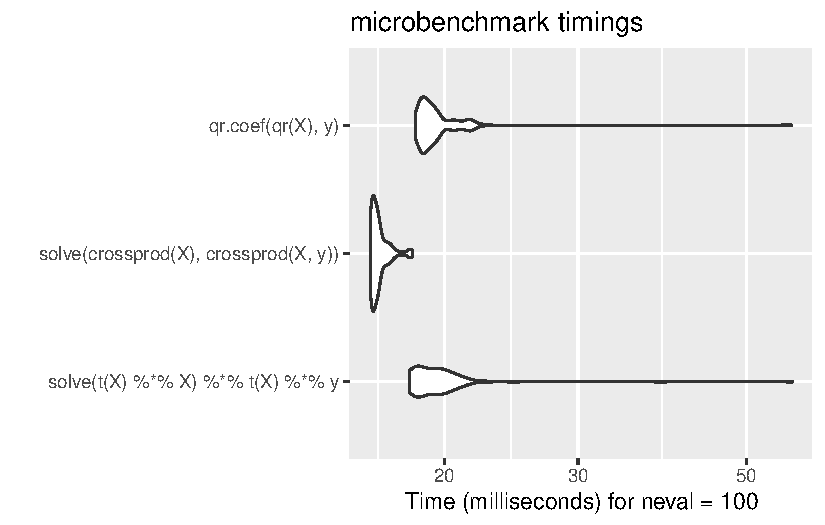
\includegraphics[keepaspectratio]{02-optimization_files/figure-pdf/unnamed-chunk-5-1.pdf}}

Compared with the approaches discussed above, this method performs
similarly to the naive approach but is much more stable and reliable.

In practice, we rarely call functions such as \texttt{qr()} or
\texttt{qr.coef()} directly, since higher-level functions like lm()
handle these computations automatically. However, in certain specialized
and performance-critical settings, it can be advantageous to use
alternative matrix decompositions to compute regression coefficients,
especially when the computation must be repeated many times in a loop
(i.e., \emph{Vectorization})

\subsection{Multivariate Normal
revisit}\label{multivariate-normal-revisit}

Computing the multivariate normal (MVN) density is a common task, for
example, when fitting spatial models or Gaussian process models. Because
maximum likelihood estimation(MLE) and likelihood ratio tests (LRT)
often require evaluating the likelihood many times, efficiency is
crucial.

After taking the log of the MVN density, we have

\[
\ell(\boldsymbol{x}\mid \boldsymbol{\mu},\Sigma) := \log \left\{ f(\boldsymbol{x}\mid \boldsymbol{\mu},\Sigma) \right\} 
= -\frac{d}{2}\log(2\pi) - \frac{1}{2}\log|\Sigma| - \frac{1}{2}(\boldsymbol{x}-\boldsymbol{\mu})^\top \Sigma^{-1}(\boldsymbol{x}-\boldsymbol{\mu}).
\] On the right hand side, the first term is a constant, the second term
is linear, and the last term is quadratic, which requires much more
computational power.

\subsubsection{A Naive Implementation}\label{a-naive-implementation}

We first center the data \(\boldsymbol{z}:=\boldsymbol{x}- \mu\). Then
we have \(\boldsymbol{z}^\top \Sigma^{-1} \boldsymbol{z}\). This
simiplified the question for a bit.

Here, much like the linear regression example above, the key bottleneck
is the inversion of the \(p\)-dimensional covariance matrix \(\Sigma\).
If we take \(\boldsymbol{z}\) to be a \(p\times 1\) column vector, then
a literal translation of the mathematics into R code might look
something like this,

\begin{Shaded}
\begin{Highlighting}[]
\FunctionTok{t}\NormalTok{(z) }\SpecialCharTok{\%*\%} \FunctionTok{solve}\NormalTok{(Sigma) }\SpecialCharTok{\%*\%}\NormalTok{ z}
\end{Highlighting}
\end{Shaded}

To illustrate, let's simulate some data and compute the quadratic form
the naive way:

\begin{Shaded}
\begin{Highlighting}[]
\FunctionTok{set.seed}\NormalTok{(}\DecValTok{2025{-}09{-}03}\NormalTok{)}

\CommentTok{\# Generate data}
\NormalTok{z }\OtherTok{\textless{}{-}} \FunctionTok{matrix}\NormalTok{(}\FunctionTok{rnorm}\NormalTok{(}\DecValTok{200} \SpecialCharTok{*} \DecValTok{100}\NormalTok{), }\DecValTok{200}\NormalTok{, }\DecValTok{100}\NormalTok{)}
\NormalTok{S }\OtherTok{\textless{}{-}} \FunctionTok{cov}\NormalTok{(z)}

\CommentTok{\# Naive quadratic form}
\NormalTok{quad.naive }\OtherTok{\textless{}{-}} \ControlFlowTok{function}\NormalTok{(z, S) \{}
\NormalTok{  Sinv }\OtherTok{\textless{}{-}} \FunctionTok{solve}\NormalTok{(S)}
  \FunctionTok{rowSums}\NormalTok{((z }\SpecialCharTok{\%*\%}\NormalTok{ Sinv) }\SpecialCharTok{*}\NormalTok{ z)}
\NormalTok{\}}

\FunctionTok{library}\NormalTok{(dplyr)}
\FunctionTok{quad.naive}\NormalTok{(z, S) }\SpecialCharTok{\%\textgreater{}\%} \FunctionTok{summary}\NormalTok{()}
\end{Highlighting}
\end{Shaded}

\begin{verbatim}
   Min. 1st Qu.  Median    Mean 3rd Qu.    Max. 
  70.67   93.61   99.94  100.54  107.31  126.73 
\end{verbatim}

\subsubsection{A Better Way: Cholesky
Decomposition}\label{a-better-way-cholesky-decomposition}

Because the covariance matrix \Sigma is symmetric and positive definite,
we can exploit its \textbf{Cholesky decomposition}. That is, we write
\(\Sigma = R^\top R\), where \(R\) is a upper triangular matrix. Then,
\[
\boldsymbol{z}^\top \Sigma^{-1} \boldsymbol{z}= \boldsymbol{z}^\top (R^\top R)^{-1} \boldsymbol{z}= \boldsymbol{z}^\top R^{-1}R^{-\top} \boldsymbol{z}= (R^{-\top}\boldsymbol{z})^\top (R^{-\top} \boldsymbol{z}) := \boldsymbol{v}^\top \boldsymbol{v}.
\] Note that \(\boldsymbol{v}\in \mathbb R^p\) is the solution to the
linear system \(R^\top \boldsymbol{v}= \boldsymbol{z}\). Because \(R\)
is upper triangular, we can solve this system efficiently using back
substitution. Also, we can solve this without doing the inversion.

Once we have \(\boldsymbol{v}\) we can compute its quadratic form
\(\boldsymbol{v}^\top \boldsymbol{v}\) by the \texttt{crossprod()}
function.

\begin{Shaded}
\begin{Highlighting}[]
\NormalTok{quad.chol }\OtherTok{\textless{}{-}} \ControlFlowTok{function}\NormalTok{(z, S) \{}
\NormalTok{  R }\OtherTok{\textless{}{-}} \FunctionTok{chol}\NormalTok{(S)}
\NormalTok{  v }\OtherTok{\textless{}{-}} \FunctionTok{backsolve}\NormalTok{(R, }\FunctionTok{t}\NormalTok{(z), }\AttributeTok{transpose =} \ConstantTok{TRUE}\NormalTok{)}
  \FunctionTok{colSums}\NormalTok{(v }\SpecialCharTok{*}\NormalTok{ v)}
\NormalTok{\}}

\FunctionTok{quad.chol}\NormalTok{(z, S) }\SpecialCharTok{\%\textgreater{}\%} \FunctionTok{summary}\NormalTok{()}
\end{Highlighting}
\end{Shaded}

\begin{verbatim}
   Min. 1st Qu.  Median    Mean 3rd Qu.    Max. 
  70.67   93.61   99.94  100.54  107.31  126.73 
\end{verbatim}

\subsubsection{By product}\label{by-product}

Another benefit of the Cholesky decomposition is that it gives us a
simple way to compute the log-determinant of \(\Sigma\). The
log-determinant of \(\Sigma\) is simply two times the sum of the log of
the diagonal elements of R. (Why?)

\subsubsection{Performance comparison}\label{performance-comparison}

\begin{Shaded}
\begin{Highlighting}[]
\FunctionTok{library}\NormalTok{(microbenchmark)}
\FunctionTok{library}\NormalTok{(ggplot2)}
\NormalTok{m2 }\OtherTok{\textless{}{-}} \FunctionTok{microbenchmark}\NormalTok{(}
  \AttributeTok{naive =} \FunctionTok{quad.naive}\NormalTok{(z, S),}
  \AttributeTok{chol  =} \FunctionTok{quad.chol}\NormalTok{(z, S)}
\NormalTok{)}
\FunctionTok{autoplot}\NormalTok{(m2)}
\end{Highlighting}
\end{Shaded}

\pandocbounded{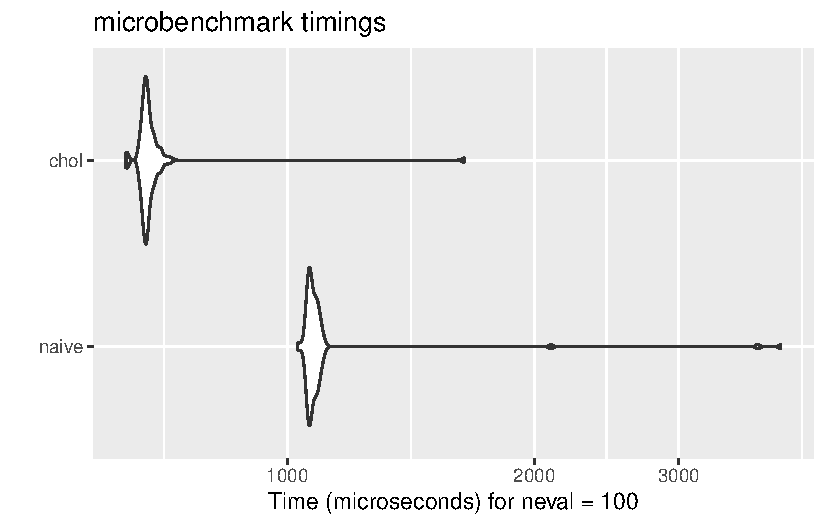
\includegraphics[keepaspectratio]{02-optimization_files/figure-pdf/unnamed-chunk-8-1.pdf}}

Q: Why one is faster than the other?

\subsubsection{Take home message 2}\label{take-home-message-2}

The naive algorithm simply inverts the covariance matrix. The
Cholesky-based approach, on the other hand, exploits the fact that
covariance matrices are symmetric and positive definite. This results in
an implementation that is both faster and numerically more
stable---exactly the kind of optimization that makes a difference in
real-world statistical computing.

Thus, a knowledge of statistics and numerical analysis can often lead to
better algorithms, often invaluable!

\begin{center}\rule{0.5\linewidth}{0.5pt}\end{center}

\section{Nonlinear functions}\label{nonlinear-functions}

On the top, we have \emph{linear functions}, such as \(y=f(x) = ax + b\)
or in the linear regression \(y=X\beta +\epsilon\). It is a small class
of the functions, and may be relatively limited.

E.g., what if we have a quadratic relationship? Then
\(y=f(x) = ax^2 + bx + c\).

Such nonlinear relationship is very common, , such as
\(f(x) = a\sin(bx + c)\) or \(f(x) = a\exp(bx) + c\), and they may not
have a closed-form solution like in the linear regression case.

From now on, we will be talking about the numerical approaches to solve
these problems.

\section{Type of Optimization
Algorithms}\label{type-of-optimization-algorithms}

There are in general two types of the optimization algorithms: (1).
\textbf{deterministic} and (2). \textbf{metaheuristic}. Deterministic
and metaheuristic algorithms represent two distinct paradigms in
optimization.

*. \textbf{Deterministic methods}: such as gradient descent, produce the
same solution for a given input and follow a predictable path toward an
optimum.

*. In contrast, \textbf{metaheuristic approaches}: incorporate
randomness and do not guarantee the best possible solution. However,
they are often more effective at avoiding local optima and exploring
complex search spaces.

\section{Deterministic Algorithms}\label{deterministic-algorithms}

Numerical approximation, what you learned in the mathematical
optimization course. Some of the algorithms include:

\begin{itemize}
\tightlist
\item
  Gradient Descent
\item
  Newton's Method
\item
  Conjugate Gradient Method
\item
  Quasi-Newton Methods (e.g., BFGS)
\item
  Interior Point Methods
\end{itemize}

They often rely on the \textbf{Karush--Kuhn--Tucker} (KKT) conditions.

\subsection{Root finding}\label{root-finding}

The \emph{root finding} is probably the first numerical approach you
learned in the numerical analysis course. Consider a function
\(f: \mathbb R\to \mathbb R\). The point \(x\in \mathbb R\) is called a
\emph{root} of \(f\) if \(f(x) = 0\).

Q: Why do we care about the root finding?

This idea has broad applications. While finding the values of x such
that f(x) = 0 is useful in many settings, a more general task is to
determine the values of x for which f(x) = y. The same techniques used
to find the roots of a function can be applied here by rewriting the
problem as \[
\tilde{f}(x) := f(x) - y = 0.
\] In this way, new function \(\tilde{f}(x)\) has a root at the solution
to, \(f(x)=y\), original equation.

For linear function, it is trivial. For quadratic function, we can use
the quadratic formula, i.e., \[
x = \frac{-b \pm \sqrt{b^2 - 4ac}}{2a}.
\] However, for more complex functions, we need to use numerical methods
to solve it iteratively. Below, we are going to go over some numerical
algorithms.

\subsection{One-dimensional case}\label{one-dimensional-case}

We first look at the one-dimensional case. The function we want to
optimize is

\[f(x) = x^3 - x + 1\]

\subsection{Bisection method}\label{bisection-method}

Bisection method is just like a \emph{binary search}.

\textbf{Step 1.} Selection two points
\(a,b\in \chi \subseteq \mathbb R\), where \(\chi\) is the domain of
\(f\). Make sure that \(a\) and \(b\) have opposite signs, i.e.,
\(f(a)f(b) < 0\).

\textbf{Step 2.} Compute the midpoint \(c = (a+b)/2\).

\textbf{Step 3.} Evaluate and check the sign of \(f(c)\). If \(f(c)\)
has the same sign as \(f(a)\), then set \(a=c\). Otherwise, set \(b=c\).

\textbf{Step 4.} Iterate Steps 2 and 3 until the interval \([a,b]\) is
sufficiently small.

The intuition here is that we are shirking the search space \(\chi\) by
half in each iteration.

Q: Why this algorithm work and what are the assumptions? 1. We require
the function to be continuous 2. We require the function to have
opposite signs at the two endpoints \(a,b\in\chi\subseteq \mathbb R\).
3. We do not require the differentiability!

Q: But what's the cost?

Q: Can this work for every function?

\subsubsection{Example}\label{example}

Suppose the design region is

\begin{Shaded}
\begin{Highlighting}[]
\NormalTok{a }\OtherTok{\textless{}{-}} \DecValTok{1}
\NormalTok{b }\OtherTok{\textless{}{-}} \DecValTok{4}
\FunctionTok{curve}\NormalTok{(}\FloatTok{0.5}\SpecialCharTok{*}\NormalTok{x}\SpecialCharTok{\^{}}\DecValTok{3} \SpecialCharTok{{-}} \FloatTok{0.5}\SpecialCharTok{*}\NormalTok{x }\SpecialCharTok{{-}} \DecValTok{18}\NormalTok{, }\AttributeTok{from =}\NormalTok{ a, }\AttributeTok{to =}\NormalTok{ b, }\AttributeTok{xlab =} \StringTok{"x"}\NormalTok{, }\AttributeTok{ylab =} \StringTok{"f(x)"}\NormalTok{)}
\NormalTok{fun\_obj }\OtherTok{\textless{}{-}} \ControlFlowTok{function}\NormalTok{(x) }\FloatTok{0.5}\SpecialCharTok{*}\NormalTok{x}\SpecialCharTok{\^{}}\DecValTok{3} \SpecialCharTok{{-}} \FloatTok{0.5}\SpecialCharTok{*}\NormalTok{x }\SpecialCharTok{{-}} \DecValTok{18}

\NormalTok{my\_bisec }\OtherTok{\textless{}{-}} \ControlFlowTok{function}\NormalTok{(fun\_obj, a, b, }\AttributeTok{tol =} \FloatTok{1E{-}2}\NormalTok{, }\AttributeTok{ind\_draw =} \ConstantTok{FALSE}\NormalTok{) \{}
  \ControlFlowTok{if}\NormalTok{ (}\FunctionTok{fun\_obj}\NormalTok{(a) }\SpecialCharTok{*} \FunctionTok{fun\_obj}\NormalTok{(b) }\SpecialCharTok{\textgreater{}} \DecValTok{0}\NormalTok{) \{}
    \FunctionTok{stop}\NormalTok{(}\StringTok{"f(a) and f(b) must have opposite signs!"}\NormalTok{)}
\NormalTok{  \}}
\NormalTok{  iter }\OtherTok{\textless{}{-}} \DecValTok{0}
  \ControlFlowTok{while}\NormalTok{ ((b }\SpecialCharTok{{-}}\NormalTok{ a) }\SpecialCharTok{/} \DecValTok{2} \SpecialCharTok{\textgreater{}}\NormalTok{ tol) \{}
\NormalTok{    c }\OtherTok{\textless{}{-}}\NormalTok{ (a }\SpecialCharTok{+}\NormalTok{ b) }\SpecialCharTok{/} \DecValTok{2}
    
    \ControlFlowTok{if}\NormalTok{ (ind\_draw }\SpecialCharTok{==} \ConstantTok{TRUE}\NormalTok{) \{}
    \CommentTok{\# Draw vertical line}
    \FunctionTok{abline}\NormalTok{(}\AttributeTok{v =}\NormalTok{ c, }\AttributeTok{col =} \StringTok{"red"}\NormalTok{, }\AttributeTok{lty =} \DecValTok{2}\NormalTok{)}
    \CommentTok{\# Label the iteration above the x{-}axis}
    \FunctionTok{text}\NormalTok{(c, }\FunctionTok{par}\NormalTok{(}\StringTok{"usr"}\NormalTok{)[}\DecValTok{3}\NormalTok{] }\SpecialCharTok{+} \DecValTok{2}\NormalTok{, }\AttributeTok{labels =}\NormalTok{ iter }\SpecialCharTok{+} \DecValTok{1}\NormalTok{, }\AttributeTok{col =} \StringTok{"blue"}\NormalTok{, }\AttributeTok{pos =} \DecValTok{3}\NormalTok{, }\AttributeTok{cex =} \FloatTok{0.8}\NormalTok{)}
\NormalTok{    \}}

    
    \ControlFlowTok{if}\NormalTok{ (}\FunctionTok{fun\_obj}\NormalTok{(c) }\SpecialCharTok{==} \DecValTok{0}\NormalTok{) \{}
      \FunctionTok{return}\NormalTok{(c)}
\NormalTok{    \} }\ControlFlowTok{else} \ControlFlowTok{if}\NormalTok{ (}\FunctionTok{fun\_obj}\NormalTok{(a) }\SpecialCharTok{*} \FunctionTok{fun\_obj}\NormalTok{(c) }\SpecialCharTok{\textless{}} \DecValTok{0}\NormalTok{) \{}
\NormalTok{      b }\OtherTok{\textless{}{-}}\NormalTok{ c}
\NormalTok{    \} }\ControlFlowTok{else}\NormalTok{ \{}
\NormalTok{      a }\OtherTok{\textless{}{-}}\NormalTok{ c}
\NormalTok{    \}}
\NormalTok{    iter }\OtherTok{\textless{}{-}}\NormalTok{ iter }\SpecialCharTok{+} \DecValTok{1}
\NormalTok{  \}}
\NormalTok{  val\_x }\OtherTok{\textless{}{-}}\NormalTok{ (a }\SpecialCharTok{+}\NormalTok{ b) }\SpecialCharTok{/} \DecValTok{2}
\NormalTok{  val\_fx }\OtherTok{\textless{}{-}} \FunctionTok{fun\_obj}\NormalTok{(val\_x)}
  \FunctionTok{return}\NormalTok{(}\FunctionTok{list}\NormalTok{(}\AttributeTok{root =}\NormalTok{ val\_x, }\AttributeTok{f\_root =}\NormalTok{ val\_fx, }\AttributeTok{iter =}\NormalTok{ iter))}
\NormalTok{\}}

\CommentTok{\# Run it}
\NormalTok{res\_plot }\OtherTok{\textless{}{-}} \FunctionTok{my\_bisec}\NormalTok{(fun\_obj, a, b, }\AttributeTok{ind\_draw =} \ConstantTok{TRUE}\NormalTok{)}
\end{Highlighting}
\end{Shaded}

\pandocbounded{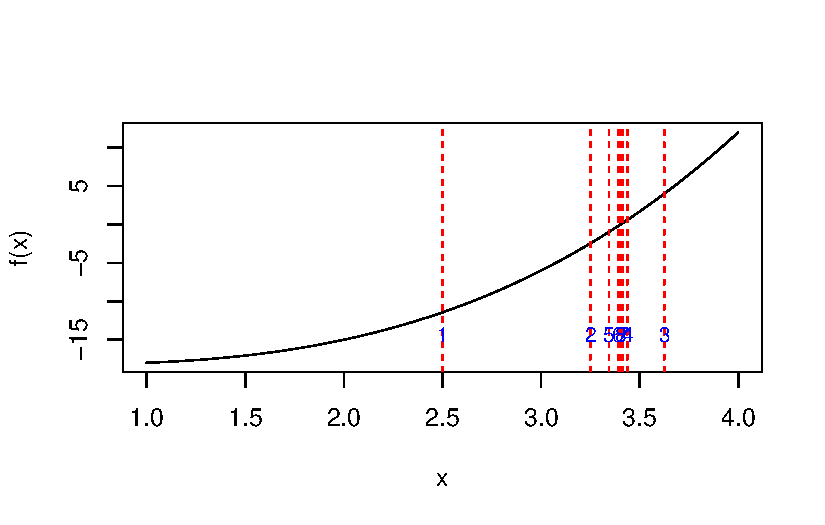
\includegraphics[keepaspectratio]{02-optimization_files/figure-pdf/unnamed-chunk-9-1.pdf}}

\begin{Shaded}
\begin{Highlighting}[]
\NormalTok{res\_plot}
\end{Highlighting}
\end{Shaded}

\begin{verbatim}
$root
[1] 3.408203

$f_root
[1] 0.09048409

$iter
[1] 8
\end{verbatim}

\begin{Shaded}
\begin{Highlighting}[]
\NormalTok{res }\OtherTok{\textless{}{-}} \FunctionTok{my\_bisec}\NormalTok{(fun\_obj, a, b)}
\FunctionTok{plot}\NormalTok{(}\ControlFlowTok{function}\NormalTok{(x) }\FunctionTok{fun\_obj}\NormalTok{(x), }\AttributeTok{from =}\NormalTok{ a, }\AttributeTok{to =}\NormalTok{ b)}
\FunctionTok{abline}\NormalTok{(}\AttributeTok{h =} \DecValTok{0}\NormalTok{, }\AttributeTok{col =} \StringTok{"blue"}\NormalTok{, }\AttributeTok{lty =} \DecValTok{2}\NormalTok{)}
\FunctionTok{title}\NormalTok{(}\AttributeTok{main =} \FunctionTok{paste0}\NormalTok{(}\StringTok{"Bisection Method with "}\NormalTok{, res}\SpecialCharTok{$}\NormalTok{iter, }\StringTok{" iterations"}\NormalTok{))}
\FunctionTok{abline}\NormalTok{(}\AttributeTok{v =}\NormalTok{ res}\SpecialCharTok{$}\NormalTok{root, }\AttributeTok{col =} \StringTok{"red"}\NormalTok{, }\AttributeTok{lwd =} \DecValTok{2}\NormalTok{)}
\FunctionTok{text}\NormalTok{(res}\SpecialCharTok{$}\NormalTok{root, }\FunctionTok{par}\NormalTok{(}\StringTok{"usr"}\NormalTok{)[}\DecValTok{3}\NormalTok{] }\SpecialCharTok{+} \DecValTok{5}\NormalTok{, }
     \AttributeTok{labels =} \FunctionTok{paste0}\NormalTok{(}\StringTok{"Root \textasciitilde{}= "}\NormalTok{, }\FunctionTok{round}\NormalTok{(res}\SpecialCharTok{$}\NormalTok{root, }\DecValTok{3}\NormalTok{)), }
     \AttributeTok{col =} \StringTok{"red"}\NormalTok{, }\AttributeTok{pos =} \DecValTok{3}\NormalTok{, }\AttributeTok{cex =} \FloatTok{0.9}\NormalTok{, }\AttributeTok{font =} \DecValTok{2}\NormalTok{)}
\end{Highlighting}
\end{Shaded}

\pandocbounded{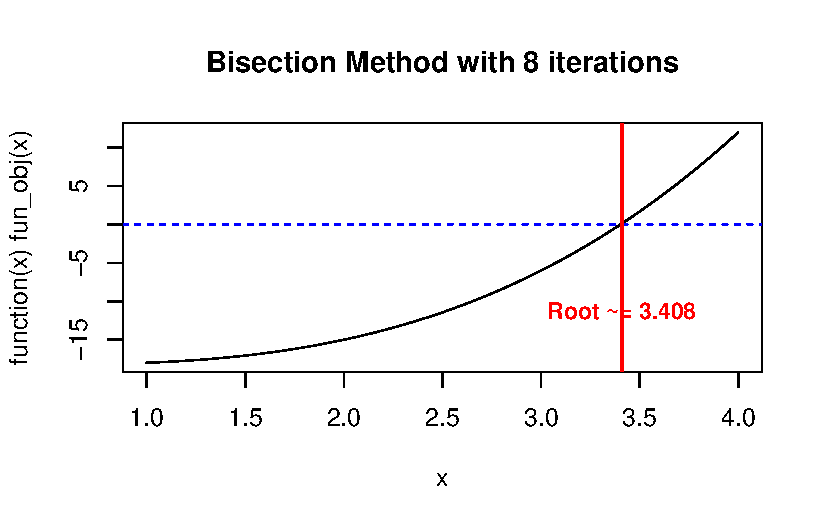
\includegraphics[keepaspectratio]{02-optimization_files/figure-pdf/unnamed-chunk-9-2.pdf}}

\subsection{Newton-Raphson method}\label{newton-raphson-method}

The Newton-Raphson method (or simply Newton's method) is an iterative
numerical method for finding successively better approximations to the
roots (or zeroes) of a real-valued function.

Here, we assume that the function \(f\) is differentiable. The idea here
is to use the Taylor expansion of the function. Suppose we are search a
small neighbour of the solution \(x \in \mathbb R\), say
\(x_j \in \mathbb R\) is a small number. Then Then we first order Taylor
series to approximate \(f(x_j+h)\) around \(x_j\) is \[
f(x)\approx f(x_j) +  f^\prime(x_j) (x-x_j),
\] where \(f^\prime(x) := \partial_x f(x)\) is the first derivative of
\(f(x)\). So the root of this approximation can be improved by updating
its place to where \(f(x_{j+1}) = 0\).

So if \(f(x_j+h)\) is the root, then we have
\[ 0 = f(x_j) + f^\prime(x_j) h \implies h = -\frac{f(x_j)}{f^\prime(x_j)}.\]

Then, we can come back to \(x_{j+1}= x_j+h\), and plug the value of
\(h\) in from above, we have \[
x_{j+1} = x_j - \frac{f(x_j)}{f^\prime(x_j)}.
\]

The algorithm is given as below:

Let \(f:\mathbb R\to\mathbb R\) be differentiable.

Step 0: Choose a function \(f(x)\): This is the function for which you
want to find a root (i.e., solve \(f(x) = 0\)).

Step 1: Calculate the derivative \(f^\prime(x)\): You will need it to
apply the formula.

Step 2: Make an initial guess \(x_0\): Select a starting point \(x_0\)
near the expected root.

Step 3: Update the estimate: Use the Newton's method formula to compute
the next estimate \(x_1\) using \(x_0\) by
\[x_{j+1} = x_j - \frac{f(x_j)}{f^\prime(x_j)}.\]

Step 4: Repeat Steps 2 and 3 until the values converge to a root or
reach a desired tolerance.

\begin{Shaded}
\begin{Highlighting}[]
\DocumentationTok{\#\# Function and derivative}
\NormalTok{f  }\OtherTok{\textless{}{-}} \ControlFlowTok{function}\NormalTok{(x) }\FloatTok{0.5}\SpecialCharTok{*}\NormalTok{x}\SpecialCharTok{\^{}}\DecValTok{3} \SpecialCharTok{{-}} \FloatTok{0.5}\SpecialCharTok{*}\NormalTok{x }\SpecialCharTok{{-}} \DecValTok{18}
\NormalTok{df }\OtherTok{\textless{}{-}} \ControlFlowTok{function}\NormalTok{(x) }\FloatTok{1.5}\SpecialCharTok{*}\NormalTok{x}\SpecialCharTok{\^{}}\DecValTok{2} \SpecialCharTok{{-}} \FloatTok{0.5}

\DocumentationTok{\#\# Newton–Raphson with iterate tracking}
\NormalTok{newton\_raphson }\OtherTok{\textless{}{-}} \ControlFlowTok{function}\NormalTok{(f, df, x0, }\AttributeTok{tol =} \FloatTok{1e{-}5}\NormalTok{, }
                           \AttributeTok{maxit =} \DecValTok{100}\NormalTok{, }\AttributeTok{eps =} \FloatTok{1e{-}5}\NormalTok{) \{}
\NormalTok{  x }\OtherTok{\textless{}{-}}\NormalTok{ x0}
\NormalTok{  xs }\OtherTok{\textless{}{-}}\NormalTok{ x0      }\CommentTok{\# store iterates (x0, x1, x2, ...)}
  \ControlFlowTok{for}\NormalTok{ (k }\ControlFlowTok{in} \DecValTok{1}\SpecialCharTok{:}\NormalTok{maxit) \{}
\NormalTok{    fx  }\OtherTok{\textless{}{-}} \FunctionTok{f}\NormalTok{(x)}
\NormalTok{    dfx }\OtherTok{\textless{}{-}} \FunctionTok{df}\NormalTok{(x)}
\NormalTok{    x\_new }\OtherTok{\textless{}{-}}\NormalTok{ x }\SpecialCharTok{{-}}\NormalTok{ fx}\SpecialCharTok{/}\NormalTok{dfx}
\NormalTok{    xs }\OtherTok{\textless{}{-}} \FunctionTok{c}\NormalTok{(xs, x\_new)}
    \ControlFlowTok{if}\NormalTok{ (}\FunctionTok{abs}\NormalTok{(x\_new }\SpecialCharTok{{-}}\NormalTok{ x) }\SpecialCharTok{\textless{}}\NormalTok{ tol }\SpecialCharTok{||} \FunctionTok{abs}\NormalTok{(fx) }\SpecialCharTok{\textless{}}\NormalTok{ tol) \{}
      \FunctionTok{return}\NormalTok{(}\FunctionTok{list}\NormalTok{(}\AttributeTok{root =}\NormalTok{ x\_new, }\AttributeTok{iter =}\NormalTok{ k, }\AttributeTok{path =}\NormalTok{ xs))}
\NormalTok{    \}}
\NormalTok{    x }\OtherTok{\textless{}{-}}\NormalTok{ x\_new}
\NormalTok{  \}}
  \FunctionTok{list}\NormalTok{(}\AttributeTok{root =}\NormalTok{ x, }\AttributeTok{iter =}\NormalTok{ maxit, }\AttributeTok{path =}\NormalTok{ xs)}
\NormalTok{\}}

\DocumentationTok{\#\# Starting point}
\end{Highlighting}
\end{Shaded}

If we start at -1 which is far away from

\begin{Shaded}
\begin{Highlighting}[]
\NormalTok{x0 }\OtherTok{\textless{}{-}} \SpecialCharTok{{-}}\DecValTok{1}
\NormalTok{res }\OtherTok{\textless{}{-}} \FunctionTok{newton\_raphson}\NormalTok{(f, df, x0)}
\NormalTok{a }\OtherTok{\textless{}{-}} \SpecialCharTok{{-}}\DecValTok{2}\NormalTok{; b }\OtherTok{\textless{}{-}} \DecValTok{5}
\FunctionTok{plot}\NormalTok{(}\ControlFlowTok{function}\NormalTok{(x) }\FunctionTok{f}\NormalTok{(x), }\AttributeTok{from =}\NormalTok{ a, }\AttributeTok{to =}\NormalTok{ b, }
     \AttributeTok{xlab =} \StringTok{"x"}\NormalTok{, }\AttributeTok{ylab =} \StringTok{"f(x)"}\NormalTok{,}
     \AttributeTok{main =} \FunctionTok{paste}\NormalTok{(}\StringTok{"Newton{-}Raphson (Iterations:"}\NormalTok{, res}\SpecialCharTok{$}\NormalTok{iter, }\StringTok{")"}\NormalTok{))}
\FunctionTok{abline}\NormalTok{(}\AttributeTok{h =} \DecValTok{0}\NormalTok{, }\AttributeTok{col =} \StringTok{"blue"}\NormalTok{, }\AttributeTok{lty =} \DecValTok{2}\NormalTok{)}

\DocumentationTok{\#\# Draw vertical lines for each iterate with labels 0,1,2,...}
\ControlFlowTok{for}\NormalTok{ (i }\ControlFlowTok{in} \FunctionTok{seq\_along}\NormalTok{(res}\SpecialCharTok{$}\NormalTok{path)) \{}
\NormalTok{  xi }\OtherTok{\textless{}{-}}\NormalTok{ res}\SpecialCharTok{$}\NormalTok{path[i]}
  \FunctionTok{abline}\NormalTok{(}\AttributeTok{v =}\NormalTok{ xi, }\AttributeTok{col =} \StringTok{"red"}\NormalTok{, }\AttributeTok{lty =} \DecValTok{2}\NormalTok{)}
  \FunctionTok{text}\NormalTok{(xi, }\FunctionTok{par}\NormalTok{(}\StringTok{"usr"}\NormalTok{)[}\DecValTok{3}\NormalTok{] }\SpecialCharTok{+} \DecValTok{2}\NormalTok{, }\AttributeTok{labels =}\NormalTok{ i }\SpecialCharTok{{-}} \DecValTok{1}\NormalTok{, }\AttributeTok{col =} \StringTok{"blue"}\NormalTok{, }\AttributeTok{pos =} \DecValTok{3}\NormalTok{, }\AttributeTok{cex =} \FloatTok{0.9}\NormalTok{)}
\NormalTok{\}}

\DocumentationTok{\#\# Final root marker + label}
\FunctionTok{abline}\NormalTok{(}\AttributeTok{v =}\NormalTok{ res}\SpecialCharTok{$}\NormalTok{root, }\AttributeTok{col =} \StringTok{"darkgreen"}\NormalTok{, }\AttributeTok{lwd =} \DecValTok{2}\NormalTok{)}
\FunctionTok{text}\NormalTok{(res}\SpecialCharTok{$}\NormalTok{root, }\FunctionTok{par}\NormalTok{(}\StringTok{"usr"}\NormalTok{)[}\DecValTok{3}\NormalTok{] }\SpecialCharTok{+} \DecValTok{5}\NormalTok{,}
     \AttributeTok{labels =} \FunctionTok{paste0}\NormalTok{(}\StringTok{"Root \textasciitilde{}= "}\NormalTok{, }\FunctionTok{round}\NormalTok{(res}\SpecialCharTok{$}\NormalTok{root, }\DecValTok{5}\NormalTok{),}
                     \StringTok{" ; f(root) \textasciitilde{}= "}\NormalTok{, }\FunctionTok{signif}\NormalTok{(}\FunctionTok{f}\NormalTok{(res}\SpecialCharTok{$}\NormalTok{root), }\DecValTok{3}\NormalTok{)),}
     \AttributeTok{col =} \StringTok{"darkgreen"}\NormalTok{, }\AttributeTok{pos =} \DecValTok{3}\NormalTok{, }\AttributeTok{cex =} \FloatTok{0.95}\NormalTok{, }\AttributeTok{font =} \DecValTok{2}\NormalTok{)}
\end{Highlighting}
\end{Shaded}

\pandocbounded{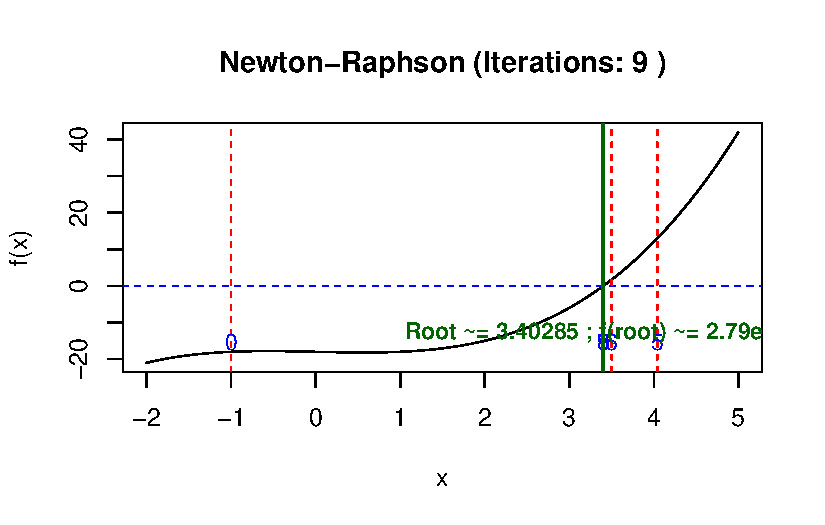
\includegraphics[keepaspectratio]{02-optimization_files/figure-pdf/unnamed-chunk-10-1.pdf}}

\begin{Shaded}
\begin{Highlighting}[]
\NormalTok{res}
\end{Highlighting}
\end{Shaded}

\begin{verbatim}
$root
[1] 3.402848

$iter
[1] 9

$path
 [1] -1.000000 17.000000 11.387991  7.704327  5.368534  4.042133  3.500619
 [8]  3.405629  3.402850  3.402848
\end{verbatim}

If we start at 3 which is near to the point

\begin{Shaded}
\begin{Highlighting}[]
\NormalTok{x0 }\OtherTok{\textless{}{-}} \DecValTok{3}
\NormalTok{res }\OtherTok{\textless{}{-}} \FunctionTok{newton\_raphson}\NormalTok{(f, df, x0)}
\DocumentationTok{\#\# Plot range that shows the iterates and root}
\NormalTok{a }\OtherTok{\textless{}{-}} \SpecialCharTok{{-}}\DecValTok{2}\NormalTok{; b }\OtherTok{\textless{}{-}} \DecValTok{5}
\FunctionTok{plot}\NormalTok{(}\ControlFlowTok{function}\NormalTok{(x) }\FunctionTok{f}\NormalTok{(x), }\AttributeTok{from =}\NormalTok{ a, }\AttributeTok{to =}\NormalTok{ b, }
     \AttributeTok{xlab =} \StringTok{"x"}\NormalTok{, }\AttributeTok{ylab =} \StringTok{"f(x)"}\NormalTok{,}
     \AttributeTok{main =} \FunctionTok{paste}\NormalTok{(}\StringTok{"Newton{-}Raphson (Iterations:"}\NormalTok{, res}\SpecialCharTok{$}\NormalTok{iter, }\StringTok{")"}\NormalTok{))}
\FunctionTok{abline}\NormalTok{(}\AttributeTok{h =} \DecValTok{0}\NormalTok{, }\AttributeTok{col =} \StringTok{"blue"}\NormalTok{, }\AttributeTok{lty =} \DecValTok{2}\NormalTok{)}

\DocumentationTok{\#\# Draw vertical lines for each iterate with labels 0,1,2,...}
\ControlFlowTok{for}\NormalTok{ (i }\ControlFlowTok{in} \FunctionTok{seq\_along}\NormalTok{(res}\SpecialCharTok{$}\NormalTok{path)) \{}
\NormalTok{  xi }\OtherTok{\textless{}{-}}\NormalTok{ res}\SpecialCharTok{$}\NormalTok{path[i]}
  \FunctionTok{abline}\NormalTok{(}\AttributeTok{v =}\NormalTok{ xi, }\AttributeTok{col =} \StringTok{"red"}\NormalTok{, }\AttributeTok{lty =} \DecValTok{2}\NormalTok{)}
  \FunctionTok{text}\NormalTok{(xi, }\FunctionTok{par}\NormalTok{(}\StringTok{"usr"}\NormalTok{)[}\DecValTok{3}\NormalTok{] }\SpecialCharTok{+} \DecValTok{2}\NormalTok{, }\AttributeTok{labels =}\NormalTok{ i }\SpecialCharTok{{-}} \DecValTok{1}\NormalTok{, }\AttributeTok{col =} \StringTok{"blue"}\NormalTok{, }\AttributeTok{pos =} \DecValTok{3}\NormalTok{, }\AttributeTok{cex =} \FloatTok{0.9}\NormalTok{)}
\NormalTok{\}}

\DocumentationTok{\#\# Final root marker + label}
\FunctionTok{abline}\NormalTok{(}\AttributeTok{v =}\NormalTok{ res}\SpecialCharTok{$}\NormalTok{root, }\AttributeTok{col =} \StringTok{"darkgreen"}\NormalTok{, }\AttributeTok{lwd =} \DecValTok{2}\NormalTok{)}
\FunctionTok{text}\NormalTok{(res}\SpecialCharTok{$}\NormalTok{root, }\FunctionTok{par}\NormalTok{(}\StringTok{"usr"}\NormalTok{)[}\DecValTok{3}\NormalTok{] }\SpecialCharTok{+} \DecValTok{5}\NormalTok{,}
     \AttributeTok{labels =} \FunctionTok{paste0}\NormalTok{(}\StringTok{"Root \textasciitilde{}= "}\NormalTok{, }\FunctionTok{round}\NormalTok{(res}\SpecialCharTok{$}\NormalTok{root, }\DecValTok{5}\NormalTok{),}
                     \StringTok{" ; f(root) \textasciitilde{}= "}\NormalTok{, }\FunctionTok{signif}\NormalTok{(}\FunctionTok{f}\NormalTok{(res}\SpecialCharTok{$}\NormalTok{root), }\DecValTok{3}\NormalTok{)),}
     \AttributeTok{col =} \StringTok{"darkgreen"}\NormalTok{, }\AttributeTok{pos =} \DecValTok{3}\NormalTok{, }\AttributeTok{cex =} \FloatTok{0.95}\NormalTok{, }\AttributeTok{font =} \DecValTok{2}\NormalTok{)}
\end{Highlighting}
\end{Shaded}

\pandocbounded{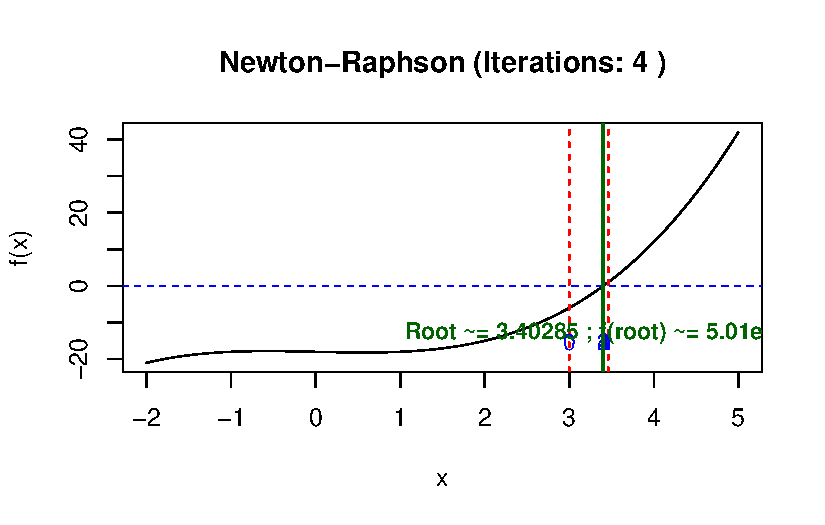
\includegraphics[keepaspectratio]{02-optimization_files/figure-pdf/unnamed-chunk-11-1.pdf}}

\begin{Shaded}
\begin{Highlighting}[]
\NormalTok{res}
\end{Highlighting}
\end{Shaded}

\begin{verbatim}
$root
[1] 3.402848

$iter
[1] 4

$path
[1] 3.000000 3.461538 3.403866 3.402848 3.402848
\end{verbatim}

Remarks:

\begin{itemize}
\item
  Assumptions: \(f\) is differentiable in a neighborhood of the root
  \(r\).
\item
  Failure cases: if \(f^\prime(x_j)=0\) (or is very small), the update
  is ill-defined/unstable; if the initial guess is far, the method can
  diverge or jump to a different root.
\item
  Practical checks: stop when \(|f(x_j)|\le \delta\) or
  \(|x_{j+1}-x_j| \le \delta\) is below tolerance \(\delta\).
\end{itemize}

\subsection{Second Method}\label{second-method}

The secant method can be thought of as a finite-difference approximation
of Newton's method, so it is considered a quasi-Newton method. It is
simialr to Newton's method, but it does not require the computation of
the derivative of the function. Instead, it approximates the derivative
using two previous points.

In the second method, we require the \textbf{first two point}s, say
\(x_0, x_1 \in \mathbb R\). Then, we can approximate the derivative of
\(f\) at \(x_1\) using the finite difference formula. Instead of
calculate the derivative \(f^\prime(x_1)\), we approximate it as using
the secant line. In calculate, we know that,
\(f^\prime(x_1) \approx \frac{f(x_1)-f(x_0)}{x_1-x_0}\), if \(x_1\) and
\(x_0\) are close. Then, we can plug this approximation into the
Newton's update formula to get
\[x_j  = x_{j-1}  - f(x_{j-1}) \frac{x_{j-1}-x_{j-2}}{f(x_{j-1}) - f(x_{j-2})} = \frac{x_{j-2} f\left(x_{j-1}\right)-x_{j-1} f\left(x_{j-2}\right)}{f\left(x_{j-1}\right)-f\left(x_{j-2}\right)} .\]

\section{Hill climbing}\label{hill-climbing}

In numerical analysis, \emph{hill climbing} is a mathematical
optimization technique which belongs to the family of \emph{local
search}. The Newton method and secant method can be thought as questions
in hill climbing.

The algorithm starts with an arbitrary solution to a problem, then
iteratively makes small changes to the solution, each time moving to a
neighboring solution that is better than the current one. The process
continues until no neighboring solution is better than the current
solution, at which point the algorithm terminates.

In the world of optimization, finding the best solution to complex
problems can be challenging, especially when the solution space is vast
and filled with local optima.

\subsection{In R}\label{in-r}

\texttt{uniroot()}, \texttt{optim()} , \texttt{nlm()}, and
\texttt{mle()} functions. Note that you may \emph{approximate the
derivative/gradient}.

\section{Converegence}\label{converegence}

In order to compare the efficiency of the set of algorithms, one may
compare \emph{their abilities} for finding the optimals. However, what
if, say, two algorithms both can find optimals, which one is better? The
\textbf{convergence rate} comes in. Convergence rate is a measure of how
quickly an iterative algorithm approaches its limit or optimal solution,
which mean, how fast the algorithm converges to the optimals.

In the previous lecture(s), we saw that we can use R functions such
\texttt{microbenchmark::microbenchmark()}, to measure the performance.
However, it may takes a long time and a lot of computational resources.
For such cases, we may use the theoretical convergence rate to compare
the efficiency of the algorithms.

The convergence rate is often classified into several categories. It
acts like the sequence \(\{x_j\}\) we learned in grade schools. Here,
\(\{x_j\}\) is a sequence of estimates generated by the algorithm at
each iterations, and \(x^*\) is the true solution or optimal value we
are trying to reach. The error at iteration \(n\) is defined as
\(e_j = d(x_j,x^*)\), where the typical metric here is the absolute
distance \(d(x_j,x^*)=|x_j-x^*|\) (note, in spaces, different metric to
define the distance). The convergence rate describes how quickly this
error sequence \(\{e_j\}\) decreases as \(j\) increases. For

\[
\lim_{j \to \infty} \frac{\left|x_{j+1}-x^* \right|}{\left|x_j-x^* \right|^q }=\mu.
\]

\subsection{Linear Convergence}\label{linear-convergence}

If order \(q = 1\) and \(0 < \mu < 1\), the sequence
\(\{x_j\}\in\mathbb R^d\) converges to \(x^*\) linearly. That is,
\(x_j\to x^*\) as \(j\to\infty\) in \(\mathbb R^d\) if there existence a
constant \(\mu\) such that \[
  \frac{\left\|x_{n+1}-x_{\infty}\right\|}{\left\|x_n-x_{\infty}\right\|} \le \mu,\quad \text{ as } \quad n\to\infty.
\] This means that the error decreases proportionally to its current
value, leading to a steady but relatively slow convergence.

\subsection{Superlinear Convergence}\label{superlinear-convergence}

Suppose \(\{x_n\}\) converges to \(x^*\), if order \(q = 1\) and
\(\mu = 0\), the sequence \(\{x_n\}\) converges to \(x^*\)
superlinearly. That is, \(x_n\) is said to be converges to \(x^*\) as
\(n\to\infty\) superlinearly if

\[
\lim _{n \to \infty} \frac{\left\|x_{n+1}-x_{\infty}\right\|}{\left\|x_n-x_{\infty}\right\|}=0.
\] It is clearly that the superlinear is a stronger condition than the
linear convergence, such that \(\mu=0\).

\subsection{Quadratic Convergence}\label{quadratic-convergence}

If order \(q = 2\) and \(\mu > 0\), the sequence \(\{x_n\}\) converges
to \(x^*\) quadratically. That is, \(x_n\) is said to be converges to
\(x^*\) as \(n\to\infty\) quadratically if

\[
\frac{\left\|x_{n+1}-x_{\infty}\right\|}{\left\|x_n-x_{\infty}\right\|^2} \le \mu, \quad \text{ as } \quad n\to\infty.
\]

\section{Heuristic Algorithms}\label{heuristic-algorithms}

Many of the heuristic algorithms are inspired by the nature, such as the
genetic algorithm (GA) and particle swarm optimization (PSO). These
algorithms are often used for complex optimization problems where
traditional methods may struggle to find a solution. Some of the popular
heuristic algorithms include:

\begin{itemize}
\tightlist
\item
  Genetic Algorithm (GA)
\item
  Particle Swarm Optimization (PSO)
\item
  Simulated Annealing (SA)
\item
  Ant Colony Optimization (ACO)
\end{itemize}

\subsection{Simulating Annealing}\label{simulating-annealing}

Simulated annealing (SA) is a \textbf{stochastic} technique for
approximating the global optimum of a given function.

Inspired by the physical process of annealing in metallurgy, Simulated
Annealing is a probabilistic technique used for solving both
combinatorial and continuous optimization problems.

What is Simulated Annealing?

Simulated Annealing is an optimization algorithm designed to search for
an optimal or near-optimal solution in a large solution space. The name
and concept are derived from the process of annealing in metallurgy,
where a material is heated and then slowly cooled to remove defects and
achieve a stable crystalline structure. In Simulated Annealing, the
``heat'' corresponds to the degree of randomness in the search process,
which decreases over time (cooling schedule) to refine the solution. The
method is widely used in combinatorial optimization, where problems
often have numerous local optima that standard techniques like gradient
descent might get stuck in. Simulated Annealing excels in escaping these
local minima by introducing controlled randomness in its search,
allowing for a more thorough exploration of the solution space.

Some terminology:

\begin{itemize}
\tightlist
\item
  Temperature: controls how likely the algorithm is to accept worse
  solutions as it explores the search space.
\end{itemize}

Step 1 (Initilization): Begin with an initial solution \(S_ο\) and an
initial temperature \(T_ο\).

Step 2 (Neighborhood Search): At step \(j\), a new solution \(S^\prime\)
is generated by making a small change (or perturbation) to \(S_j\).

Step 3 (Evaluation): evaluate the objective function \(f(S^\prime)\)
Step 3.1: If \(f^(S^\prime)\) is \emph{better} than \(f(S_j)\), we
\emph{accept} it and take it as \(S_{j+1}\). Step 3.2: If
\(f(S^\prime)\) is \emph{worse} than \(f(S_j)\), we may still accept it
with a certain probability \(P(S_{j+1}=S^\prime)=\exp(-\Delta E/T_j)\),
where \(E\) is the energy \(f(S^\prime)-f(S_j)\).

Step 4 Cooling Schedule: Decrease the temperature according to a cooling
schedule, e.g., \(T_{j+1} = \alpha T_j\) where \(\alpha \in (0,1)\) is a
cooling rate.

Step 5 (Evaluation): Repeat Steps 2 and 3 for a certain number of
iterations or until convergence criteria are met.

Example:

Figure 1 in \href{https://arxiv.org/pdf/2405.02983}{my paper}

Advantages:

\begin{itemize}
\item
  Global optimization
\item
  Flexibility
\item
  Intuitive
\item
  Derivative?
\end{itemize}

Limitations:

\begin{itemize}
\item
  Parameter semsitivity
\item
  Computational time
\item
  Slow convergence
\end{itemize}

\subsubsection{R implementation}\label{r-implementation}

An paper about an implementation in R by
\href{https://www.maths.bris.ac.uk/R/web/packages/optimization/vignettes/vignette_master.pdf}{Husmann
et al.} and another package called
\href{https://cran.r-project.org/web/packages/GenSA/GenSA.pdf}{GenSA}.

\section{Genetic Algorthm}\label{genetic-algorthm}

Genetic Algorithm (GA) is a metaheuristic optimization technique
inspired by the process of natural evolution/selection.

GA are based on an analogy with the genetic structure and behavior of
chromosomes of the population.

STEP 1: Start with an initial generation \(G_0\) of potential solutions
(individuals). Each individual is represented by a chromosome, which is
typically encoded as a binary string, real-valued vector, or other
suitable representation. Evaluate the objective function on those
points.

Step 2: Generate the next generation \(G_{j+1}\) from the current
generation \(G_j\) using genetic operators: a). Selection: Retain the
individual that is considered as \emph{good} b). Crossover: Create
children variables from the parents c). Mutation

Step 3: Repeat Step 2 until the algorithm converges or reaches a
stopping criterion.

\subsection{Particle Swarm
Optimization}\label{particle-swarm-optimization}

Particle Swarm Optimization (PSO) was proposed by Kennedy and Eberhart
in 1995. It is inspried by the movement of the species in nature, such
as fishes or birds.

The algorithm is based on a \emph{population}, not a single current
point.

At iteration \(n\) of the algorithm, a particle has a velocity \(v(n)\)
that depends on the follows.

\begin{itemize}
\item
  The location of the best objective function value that it has
  encountered, \(s(n)\).
\item
  The location of the best objective function value among its neighbors,
  \(g(n)\).
\item
  The previous velocity \(v(n – 1)\).
\end{itemize}

The position of a particle x(n) updates according to its velocity:
\[x(n+1)=x(n)+v(n),\] adjusted to stay within the bounds. The velocity
of a particle updates approximately according to this equation:

\[v(n+1) = W(n)v(n)+r(1)(s(n)−x(n))+r(2)(g(n)−x(n)).\]

Here, \(r(1),r(2) \in [0,1]\) are random scalar values, and \(W(n)\) is
an \emph{inertia factor} that adjusts during the iterations. The full
algorithm uses randomly varying neighborhoods and includes modifications
when it encounters an improving point.

Note: There are A LOT of variations of the PSO and other swarm-based
algorithms used in the literature.

In R, there is a PSO implementation in the \texttt{pso} package. The
associated manual may be found
\href{https://cran.r-project.org/web/packages/pso/pso.pdf}{here}.

\begin{center}\rule{0.5\linewidth}{0.5pt}\end{center}

Examples are borrowed from the following sources:

\begin{itemize}
\tightlist
\item
  Peng, R.D. \href{https://bookdown.org/rdpeng/advstatcomp/}{Advanced
  Statistical Computing}.
\end{itemize}

\bookmarksetup{startatroot}

\chapter{Generating Random Variables}\label{generating-random-variables}

\newcommand{\unif}{\operatorname{Unif}}
\newcommand{\geom}{\operatorname{Geom}}
\newcommand{\beta}{\operatorname{Beta}}
\newcommand{\bern}{\operatorname{Bern}}
\newcommand{\R}{\mathbb{R}}
\newcommand{\iid}{\overset{iid}{\sim}}
\newcommand{\cov}{\mathbb{C}ov}

One of the fundamental tools required in computational statistics is the
ability to \emph{simulate random variables} (rvs) from specified
probability distributions.

\section{Overview}\label{overview}

In the simplest case, to simulate drawing an observation at random from
a finite population, a method of generating rvs from the discrete
uniform distribution is required. Therefore, a suitable generator of
uniform pseudo-random numbers is essential.

Methods for generating random variates from other probability
distributions all depend on the uniform random number generator (RNG).

In the Appendices, we have seen that how to use the built-in R functions
to generate RVs from some common distributions, such as
\texttt{runif()}, \texttt{rnorm()}, \texttt{rbinom()}, etc. In this
Section, we will go over some of the common methods to generate RVs from
a costume distributions.

Example Theorem

If we already have a finite population of size \(N\) with values
\(x_1, x_2, \ldots, x_N\) in hand, we can sample from this population
\emph{with} and \emph{without} replacement.

\begin{Shaded}
\begin{Highlighting}[]
\FunctionTok{set.seed}\NormalTok{(}\DecValTok{777}\NormalTok{)}
\FunctionTok{sample}\NormalTok{(}\FunctionTok{c}\NormalTok{(}\DecValTok{0}\NormalTok{,}\DecValTok{1}\NormalTok{), }\AttributeTok{size =} \DecValTok{10}\NormalTok{, }\AttributeTok{replace =} \ConstantTok{TRUE}\NormalTok{)  }\CommentTok{\# with replacement}
\end{Highlighting}
\end{Shaded}

\begin{verbatim}
 [1] 1 0 1 1 1 1 0 1 1 1
\end{verbatim}

\begin{Shaded}
\begin{Highlighting}[]
\CommentTok{\# Lottery ticket}
\FunctionTok{sample}\NormalTok{(}\DecValTok{1}\SpecialCharTok{:}\DecValTok{999999}\NormalTok{, }\AttributeTok{size =} \DecValTok{5}\NormalTok{, }\AttributeTok{replace =} \ConstantTok{FALSE}\NormalTok{)}
\end{Highlighting}
\end{Shaded}

\begin{verbatim}
[1] 567561 203418 450070 287692 435311
\end{verbatim}

\begin{Shaded}
\begin{Highlighting}[]
\FunctionTok{sample}\NormalTok{(}\FunctionTok{toupper}\NormalTok{(letters))}
\end{Highlighting}
\end{Shaded}

\begin{verbatim}
 [1] "H" "N" "J" "Y" "B" "U" "F" "P" "Z" "V" "W" "I" "L" "A" "G" "Q" "X" "D" "M"
[20] "R" "C" "T" "O" "K" "E" "S"
\end{verbatim}

\begin{longtable}[]{@{}llll@{}}
\caption{Common probability distributions and their corresponding R
functions for cumulative distribution function (CDF) and random number
generation (borrowed from Table 3.1 in reference
{[}2{]}).}\label{tbl-my-table}\tabularnewline
\toprule\noalign{}
Distribution & cdf & Generator & Parameters \\
\midrule\noalign{}
\endfirsthead
\toprule\noalign{}
Distribution & cdf & Generator & Parameters \\
\midrule\noalign{}
\endhead
\bottomrule\noalign{}
\endlastfoot
beta & pbeta & rbeta & shape1, shape2 \\
binomial & pbinom & rbinom & size, prob \\
chi-squared & pchisq & rchisq & df \\
exponential & pexp & rexp & rate \\
F & pf & rf & df1, df2 \\
gamma & pgamma & rgamma & shape, rate or scale \\
geometric & pgeom & rgeom & prob \\
lognormal & plnorm & rlnorm & meanlog, sdlog \\
negative binomial & pnbinom & rnbinom & size, prob \\
normal & pnorm & rnorm & mean, sd \\
Poisson & ppois & rpois & lambda \\
Student's t & pt & rt & df \\
uniform & punif & runif & min, max \\
\end{longtable}

\section{Inverse Transformation
Method}\label{inverse-transformation-method}

The first method to simulate rvs is the \emph{inverse transformation
method} (ITM).

If \(X\sim F_X\) is a continuous rv, then the rv
\(U = F_X(x) \sim \operatorname{Unif}(0,1)\).

ITM of generating rvs applies the probability integral transformation.
Define the inverse transformation
\[ F^{−1}_X(u) = \inf\{x : F_X(x) = u\},\quad  0 < u < 1.\] Then, if
\(U \sim \operatorname{Unif}(0,1)\), the rv \(X = F^{−1}_X(U)\) has the
distribution \(F_X\). This can be shown as, for all \(x \in R\)
\begin{align}
P\left(F_X^{-1}(U) \leq x\right) & =P\left(\inf \left\{t: F_X(t)=U\right\} \leq x\right) \\
& =P\left(U \leq F_X(x)\right) \\
& =F_U\left(F_X(x)\right)=F_X(x),
\end{align}

Hence, \(F_X^{-1}(U)\) and \(X\) have the same distribution. So, in
order to generate rv \(X\), we can simulate
\(U\sim \operatorname{Unif}(0,1)\) first, then apply the inverse
\(F_X^{-1}(u)\).

\begin{tcolorbox}[enhanced jigsaw, colbacktitle=quarto-callout-note-color!10!white, coltitle=black, opacityback=0, toprule=.15mm, titlerule=0mm, breakable, bottomtitle=1mm, bottomrule=.15mm, colframe=quarto-callout-note-color-frame, leftrule=.75mm, rightrule=.15mm, arc=.35mm, title=\textcolor{quarto-callout-note-color}{\faInfo}\hspace{0.5em}{Procedure with inverse transformation method}, left=2mm, opacitybacktitle=0.6, toptitle=1mm, colback=white]

Given a distribution function \(F_X(\cdot)\), we can simulate/generate a
rv \(X\) using the ITM in \textbf{three} steps:

\begin{enumerate}
\def\labelenumi{\arabic{enumi}.}
\item
  Derive the inverse function \(F_X^{-1}(u)\).
\item
  Write a (\textbf{R}) command or function to compute \(F_X^{-1}(u)\).
\item
  For each random variate required:

  \begin{enumerate}
  \def\labelenumii{\roman{enumii})}
  \tightlist
  \item
    Generate a random \(u\sim \operatorname{Unif}(0,1)\).
  \item
    Obtain \(x = F_X^{-1}(u)\).
  \end{enumerate}
\end{enumerate}

\end{tcolorbox}

\subsection{Continuous case}\label{continuous-case}

When the distribution function \(F_X(\cdot)\) is continuous, the ITM is
straightforward to implement.

Suppose we want to use the ITM to simulate \(N=1000\) rvs from the
density \(f_X(x)=3x^2,\quad x\in(0,1)\).

\begin{enumerate}
\def\labelenumi{\arabic{enumi}.}
\item
  The cdf is \(F_X(x)=x^3\), so the inverse function is
  \(F_X^{-1}(u)=u^{1/3}\).
\item
  Simulate \(N=1000\) rvs from \(u\sim\operatorname{Unif}(0,1)\) and
  apply the inverse function to obtain the 1000 \(x\) values.
\end{enumerate}

\begin{Shaded}
\begin{Highlighting}[]
\FunctionTok{set.seed}\NormalTok{(}\DecValTok{777}\NormalTok{)}
\NormalTok{N }\OtherTok{\textless{}{-}} \DecValTok{1000}
\NormalTok{uVec }\OtherTok{\textless{}{-}} \FunctionTok{runif}\NormalTok{(N)}
\NormalTok{xVec }\OtherTok{\textless{}{-}}\NormalTok{ uVec}\SpecialCharTok{\^{}}\NormalTok{(}\DecValTok{1}\SpecialCharTok{/}\DecValTok{3}\NormalTok{)}

\NormalTok{df }\OtherTok{\textless{}{-}} \FunctionTok{data.frame}\NormalTok{(}\AttributeTok{x =}\NormalTok{ xVec)}

\CommentTok{\# Density histogram with theoretical density overlay}
\FunctionTok{ggplot}\NormalTok{(df, }\FunctionTok{aes}\NormalTok{(x)) }\SpecialCharTok{+}
  \FunctionTok{geom\_histogram}\NormalTok{(}\FunctionTok{aes}\NormalTok{(}\AttributeTok{y =}\NormalTok{ ..density..), }\AttributeTok{bins =} \DecValTok{30}\NormalTok{,}
                 \AttributeTok{fill =} \StringTok{"lightblue"}\NormalTok{, }\AttributeTok{color =} \StringTok{"black"}\NormalTok{) }\SpecialCharTok{+}
  \FunctionTok{stat\_function}\NormalTok{(}\AttributeTok{fun =} \ControlFlowTok{function}\NormalTok{(x) }\DecValTok{3}\SpecialCharTok{*}\NormalTok{x}\SpecialCharTok{\^{}}\DecValTok{2}\NormalTok{,}
                \AttributeTok{color =} \StringTok{"red"}\NormalTok{, }\AttributeTok{size =} \DecValTok{1}\NormalTok{) }\SpecialCharTok{+}
  \FunctionTok{labs}\NormalTok{(}\AttributeTok{title =} \FunctionTok{expression}\NormalTok{(}\FunctionTok{f}\NormalTok{(x) }\SpecialCharTok{==} \DecValTok{3}\SpecialCharTok{*}\NormalTok{x}\SpecialCharTok{\^{}}\DecValTok{2}\NormalTok{),}
       \AttributeTok{y =} \StringTok{"Density"}\NormalTok{, }\AttributeTok{x =} \StringTok{"x"}\NormalTok{) }\SpecialCharTok{+} \FunctionTok{theme\_minimal}\NormalTok{()}
\end{Highlighting}
\end{Shaded}

\pandocbounded{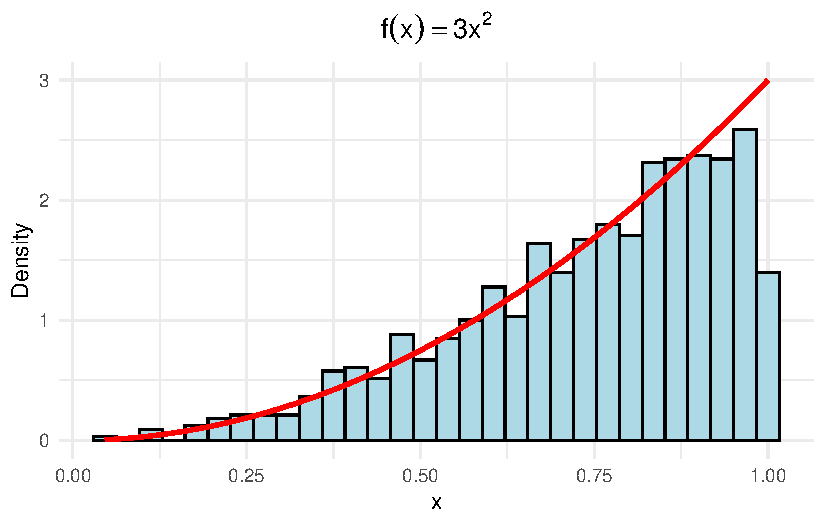
\includegraphics[keepaspectratio]{03-generating-rv_files/figure-pdf/example2-1.pdf}}

Suppose \(X\sim \exp(\lambda)\) where \(\lambda\) is the rate parameter.
Then \(F_X(x) = 1 - e^{-\lambda x}\), so the inverse function is
\(F_X^{-1}(u) = -\frac{1}{\lambda}\log(1-u)\). The other fact, is the
\(U\) and \(1-U\) have the same distribution, so we can use either of
them, i.e., \(x= -\frac{1}{\lambda}\log(u)\) or
\(x= -\frac{1}{\lambda}\log(1-u)\).

\begin{Shaded}
\begin{Highlighting}[]
\FunctionTok{set.seed}\NormalTok{(}\DecValTok{777}\NormalTok{)}
\NormalTok{N }\OtherTok{\textless{}{-}} \DecValTok{1000}
\NormalTok{lambda }\OtherTok{\textless{}{-}} \FloatTok{0.7}
\NormalTok{uVec }\OtherTok{\textless{}{-}} \FunctionTok{runif}\NormalTok{(N)}
\NormalTok{xVec\_1 }\OtherTok{\textless{}{-}} \SpecialCharTok{{-}}\NormalTok{ (}\DecValTok{1}\SpecialCharTok{/}\NormalTok{lambda) }\SpecialCharTok{*} \FunctionTok{log}\NormalTok{(uVec)}
\NormalTok{xVec\_2 }\OtherTok{\textless{}{-}} \SpecialCharTok{{-}}\NormalTok{ (}\DecValTok{1}\SpecialCharTok{/}\NormalTok{lambda) }\SpecialCharTok{*} \FunctionTok{log}\NormalTok{(}\DecValTok{1}\SpecialCharTok{{-}}\NormalTok{uVec)}

\CommentTok{\# Put data into long format for ggplot}
\NormalTok{df }\OtherTok{\textless{}{-}} \FunctionTok{data.frame}\NormalTok{(}
  \AttributeTok{value =} \FunctionTok{c}\NormalTok{(xVec\_1, xVec\_2),}
  \AttributeTok{method =} \FunctionTok{rep}\NormalTok{(}\FunctionTok{c}\NormalTok{(}\StringTok{"log(U)"}\NormalTok{, }\StringTok{"log(1{-}U)"}\NormalTok{), }\AttributeTok{each =}\NormalTok{ N)}
\NormalTok{)}

\CommentTok{\# Theoretical density function}
\NormalTok{exp\_density }\OtherTok{\textless{}{-}} \ControlFlowTok{function}\NormalTok{(x) lambda }\SpecialCharTok{*} \FunctionTok{exp}\NormalTok{(}\SpecialCharTok{{-}}\NormalTok{lambda }\SpecialCharTok{*}\NormalTok{ x)}

\CommentTok{\# Plot}
\FunctionTok{ggplot}\NormalTok{(df, }\FunctionTok{aes}\NormalTok{(}\AttributeTok{x =}\NormalTok{ value, }\AttributeTok{fill =}\NormalTok{ method)) }\SpecialCharTok{+}
  \FunctionTok{geom\_histogram}\NormalTok{(}\FunctionTok{aes}\NormalTok{(}\AttributeTok{y =}\NormalTok{ ..density..), }\AttributeTok{bins =} \DecValTok{40}\NormalTok{,}
                 \AttributeTok{position =} \StringTok{"identity"}\NormalTok{, }\AttributeTok{alpha =} \FloatTok{0.4}\NormalTok{, }\AttributeTok{color =} \StringTok{"black"}\NormalTok{) }\SpecialCharTok{+}
  \FunctionTok{stat\_function}\NormalTok{(}\AttributeTok{fun =}\NormalTok{ exp\_density, }\AttributeTok{color =} \StringTok{"red"}\NormalTok{, }\AttributeTok{size =} \DecValTok{1}\NormalTok{) }\SpecialCharTok{+}
  \FunctionTok{labs}\NormalTok{(}\AttributeTok{title =} \FunctionTok{bquote}\NormalTok{(}\StringTok{"Exponential("} \SpecialCharTok{\textasciitilde{}}\NormalTok{ lambda }\SpecialCharTok{==}\NormalTok{ .(lambda) }\SpecialCharTok{\textasciitilde{}} \StringTok{")"}\NormalTok{),}
       \AttributeTok{x =} \StringTok{"x"}\NormalTok{, }\AttributeTok{y =} \StringTok{"Density"}\NormalTok{) }
\end{Highlighting}
\end{Shaded}

\pandocbounded{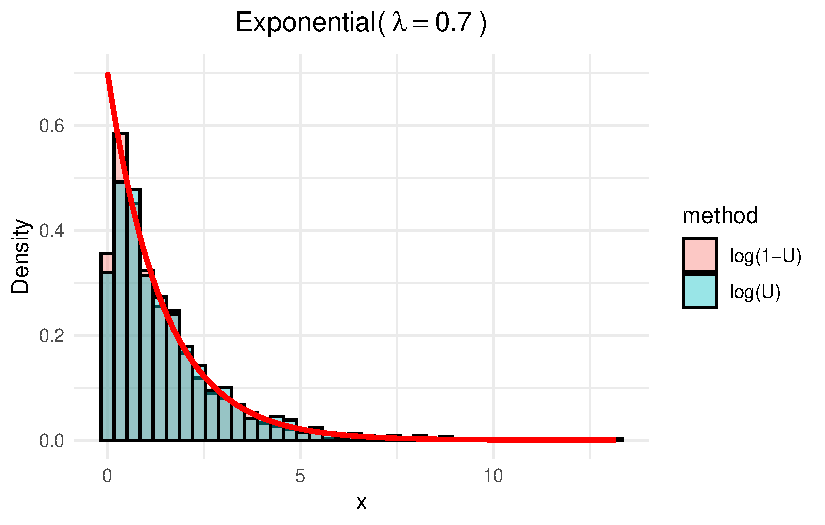
\includegraphics[keepaspectratio]{03-generating-rv_files/figure-pdf/example-exponential-1.pdf}}

\subsection{Discrete case}\label{discrete-case}

Although it is slightly more complicated than the continuous case, the
ITM can also be applied to \emph{discrete distributions}. Why?

First, in the discrete case, the cdf \(F_X(x)\) is \textbf{NOT
continuous}, instead, a step function, so the inverse function
\(F_X^{-1}(u)\) is not unique.

Here, if we order the random variable
\[\cdots < x_{(i-1)} < x_{(i)} < x_{(i+1)}< cdots,\] then the inverse
transformation is \(F_X^{-1}(u)=x_i\), where
\(F_X(x_{(i-1)}) < u \leq F_X(x_{(i)})\).

Then the procedure is:

\begin{tcolorbox}[enhanced jigsaw, colbacktitle=quarto-callout-note-color!10!white, coltitle=black, opacityback=0, toprule=.15mm, titlerule=0mm, breakable, bottomtitle=1mm, bottomrule=.15mm, colframe=quarto-callout-note-color-frame, leftrule=.75mm, rightrule=.15mm, arc=.35mm, title=\textcolor{quarto-callout-note-color}{\faInfo}\hspace{0.5em}{Procedure with ITM for discrete case}, left=2mm, opacitybacktitle=0.6, toptitle=1mm, colback=white]

\begin{enumerate}
\def\labelenumi{\arabic{enumi}.}
\item
  Derive the cdf \(F_X(x)\) and tabulate the values of \(x_i\) and
  \(F_X(x_i)\).
\item
  Write a (\textbf{R}) command or function to compute \(F_X^{-1}(u)\).
\item
  For each random variate required:

  \begin{enumerate}
  \def\labelenumii{\roman{enumii})}
  \tightlist
  \item
    Generate a random \(u\sim \operatorname{Unif}(0,1)\).
  \item
    Find \(x_i\) such that \(F_X(x_{(i-1)}) < u \leq F_X(x_{(i)})\) and
    set \(x = x_i\).
  \end{enumerate}
\end{enumerate}

\end{tcolorbox}

In this example, \(F_X(0) = f_X(0) = 1 - p\) and \(F_X(1) = 1\).

Thus, \[
F_X^{-1}(u) = 
\begin{cases}
1, & u > 0.6,\\
0, & u \leq 0.6.
\end{cases}
\]

The generator should therefore deliver the numerical value of the
logical expression \(u > 0.6\).

\begin{Shaded}
\begin{Highlighting}[]
\FunctionTok{set.seed}\NormalTok{(}\DecValTok{777}\NormalTok{)}
\NormalTok{n }\OtherTok{\textless{}{-}} \DecValTok{1000}
\NormalTok{p }\OtherTok{\textless{}{-}} \FloatTok{0.4}
\NormalTok{u }\OtherTok{\textless{}{-}} \FunctionTok{runif}\NormalTok{(n)}
\NormalTok{x }\OtherTok{\textless{}{-}} \FunctionTok{as.integer}\NormalTok{(u }\SpecialCharTok{\textgreater{}} \FloatTok{0.6}\NormalTok{)  }\CommentTok{\# (u \textgreater{} 0.6) is a logical vector}

\NormalTok{(m\_x }\OtherTok{\textless{}{-}} \FunctionTok{mean}\NormalTok{(x));  (v\_x }\OtherTok{\textless{}{-}} \FunctionTok{var}\NormalTok{(x))}
\end{Highlighting}
\end{Shaded}

\begin{verbatim}
[1] 0.381
\end{verbatim}

\begin{verbatim}
[1] 0.2360751
\end{verbatim}

Compare the sample statistics with the theoretical moments. The sample
mean of a generated sample should be approximately \(p = 0.4\) and the
sample variance should be approximately \(p(1 - p) = 0.24\), versus our
simulated values 0.381 and 0.2360751.

In this example, we will use ITM to simulate
\(X\sim \operatorname{Geom}(1/4)\).

Let \(q:=1-p\). The pmf is \(f(x) = p q^x\), \(x = 0,1,2,\ldots\). At
the points of discontinuity \(x = 0,1,2,\ldots\), the cdf is \[
F(x) = 1 - q^{x+1}.
\] For each sample element we need to generate a
\(u\sim \operatorname{Unif}(0,1)\) and solve \[
1 - q^x < u \leq 1 - q^{x+1}.
\]

Which is equivalent to \(x < \frac{\log(1 - u)}{\log(q)} \leq x+1.\) The
solution is \[
x + 1 = \left\lceil \frac{\log(1 - u)}{\log(q)} \right\rceil,
\] where \(\lceil \cdot \rceil\) denotes the ceiling function (and
\(\lfloor \cdot \rfloor\) is the floor function). Hence, we have,

\begin{Shaded}
\begin{Highlighting}[]
\FunctionTok{set.seed}\NormalTok{(}\DecValTok{999}\NormalTok{)}
\NormalTok{n }\OtherTok{\textless{}{-}} \DecValTok{1000}
\NormalTok{p }\OtherTok{\textless{}{-}} \FloatTok{0.25}
\NormalTok{u }\OtherTok{\textless{}{-}} \FunctionTok{runif}\NormalTok{(n)}
\NormalTok{k1 }\OtherTok{\textless{}{-}} \FunctionTok{ceiling}\NormalTok{(}\FunctionTok{log}\NormalTok{(}\DecValTok{1}\SpecialCharTok{{-}}\NormalTok{u) }\SpecialCharTok{/} \FunctionTok{log}\NormalTok{(}\DecValTok{1}\SpecialCharTok{{-}}\NormalTok{p)) }\SpecialCharTok{{-}} \DecValTok{1}
\end{Highlighting}
\end{Shaded}

Note again that \(U\) and \(1 - U\) have the same distribution. Also,
the probability that \(\log(1 - u)/\log(1 - p)\) equals an integer is
zero. Thus, we can simplify it to

\begin{Shaded}
\begin{Highlighting}[]
\NormalTok{k2 }\OtherTok{\textless{}{-}} \FunctionTok{floor}\NormalTok{(}\FunctionTok{log}\NormalTok{(u) }\SpecialCharTok{/} \FunctionTok{log}\NormalTok{(}\DecValTok{1}\SpecialCharTok{{-}}\NormalTok{p))}
\NormalTok{df }\OtherTok{\textless{}{-}} \FunctionTok{data.frame}\NormalTok{(}
  \AttributeTok{value =} \FunctionTok{c}\NormalTok{(k1, k2),}
  \AttributeTok{group =} \FunctionTok{rep}\NormalTok{(}\FunctionTok{c}\NormalTok{(}\StringTok{"k1"}\NormalTok{, }\StringTok{"k2"}\NormalTok{), }\AttributeTok{each =} \FunctionTok{length}\NormalTok{(k1))}
\NormalTok{)}

\CommentTok{\# Plot both histograms side by side}
\FunctionTok{ggplot}\NormalTok{(df, }\FunctionTok{aes}\NormalTok{(}\AttributeTok{x =}\NormalTok{ value, }\AttributeTok{fill =}\NormalTok{ group)) }\SpecialCharTok{+}
  \FunctionTok{geom\_histogram}\NormalTok{(}\AttributeTok{alpha =} \FloatTok{0.6}\NormalTok{, }\AttributeTok{position =} \StringTok{"identity"}\NormalTok{, }\AttributeTok{bins =} \DecValTok{40}\NormalTok{, }\AttributeTok{color =} \StringTok{"black"}\NormalTok{) }\SpecialCharTok{+}
  \FunctionTok{labs}\NormalTok{(}\AttributeTok{title =} \StringTok{"Histograms of k1 and k2"}\NormalTok{, }\AttributeTok{x =} \StringTok{"Value"}\NormalTok{, }\AttributeTok{y =} \StringTok{"Count"}\NormalTok{) }\SpecialCharTok{+} 
  \FunctionTok{theme\_minimal}\NormalTok{()}
\end{Highlighting}
\end{Shaded}

\pandocbounded{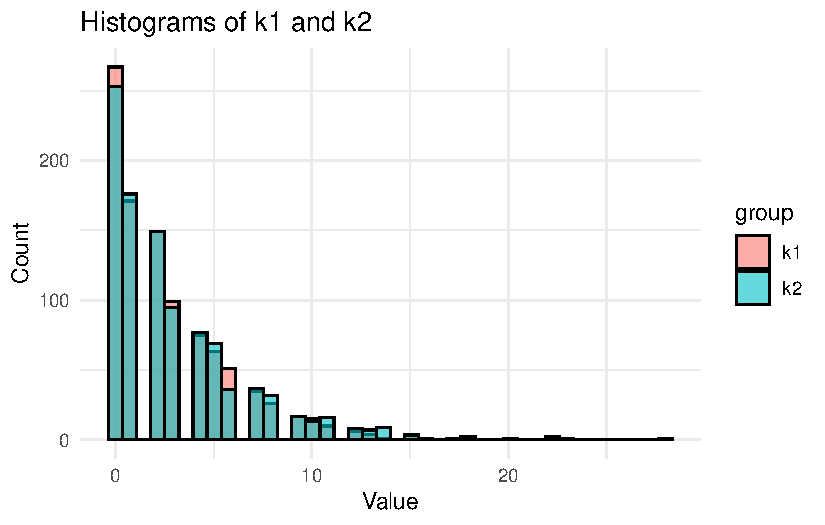
\includegraphics[keepaspectratio]{03-generating-rv_files/figure-pdf/geom2-1.pdf}}

The geometric distribution was particularly easy to simulate by the
inverse transform method because it was easy to solve the inequality {[}
F(x-1) \textless{} u \leq F(x) {]} rather than compare each \(u\) to all
the possible values \(F(x)\). \medskip

The same method applied to the Poisson distribution is more complicated
because we do not have an explicit formula for the value of \(x\) such
that \[
F(x-1) < u \leq F(x).
\]

The R function \texttt{rpois} generates random Poisson samples. The
basic method to generate a Poisson(\(\lambda\)) variate is to generate
and store the cdf via the recursive formula \[
f(x+1) = \frac{\lambda f(x)}{x+1}, 
\qquad 
F(x+1) = F(x) + f(x+1).
\]

\section{Acceptance-Rejection Method}\label{acceptance-rejection-method}

In the previous section, we have seen that the ITM is straightforward to
implement when the inverse cdf is available in closed form. However, for
many distributions, the \emph{inverse cdf is not available in closed
form or is difficult to compute}. In those cases, we need to have other
strategies!

The \emph{acceptance-rejection method} (ARM) is a general method for
generating rvs from a distribution with pdf \(f_X(x)\), when the inverse
cdf is not available in closed form or is difficult to compute.

Suppose \(X\) and \(Y\) are rvs with pdfs/pmds \(f_X(x)\) and
\(g_Y(y)\), respectively. Further we suppose there is a constant \(k\)
such that \[
\frac{f_X(t)}{g_Y(t)} \leq k,
\] for all \(t\) such that \(f_X(t) > 0\).

Then we can simulate \(X\) using the following procedure:

\begin{enumerate}
\def\labelenumi{\arabic{enumi}.}
\item
  Find a rv \(Y\) with density \(g_Y(\cdot)\) satisfying
  \(f_X(t)/g_Y(t) \le k,\) for all \(t\) such that \(f(t) > 0\).
\item
  For each rv, required:

  \begin{enumerate}
  \def\labelenumii{(\roman{enumii})}
  \tightlist
  \item
    Generate a random \(y\) from the distribution with density \(g_Y\).
  \item
    Generate a random \(u\sim \operatorname{Unif}(0,1)\).
  \item
    If \(u < f_X(y)/(k g_Y(y))\), accept \(y\) and set \(x = y\); o.w.
    reject \(y\) and jump back to (i)
  \end{enumerate}
\end{enumerate}

Why it work?Note that in Step 2c, \[
P(\text{accept} \mid Y) 
= P\!\left(U < \frac{f(Y)}{k g(Y)} \,\Big|\, Y\right) 
= \frac{f_X(Y)}{k g_X(Y)}.
\]

The total probability of acceptance for any iteration is therefore \[
\sum_y P(\text{accept} \mid y) P(Y = y) 
= \sum_y \frac{f(y)}{k g(y)} g(y) 
= \frac{1}{k},
\] and the number of iterations until acceptance has the geometric
distribution with mean \(k\). That means, in order to sample \(X\), in
average, we need \(k\) iterations.

Note: The choice of \(Y\) and \(k\) is crucial for the efficiency of the
ARM. A poor choice can lead to a large \(k\), resulting in many
rejections and inefficiency. We want \(Y\) to be easy to simulate, and
\(k\) to be as small as possible.

Does this have anything to do with \(X\)?

To see that the accepted sample has the same distribution as \(X\),
apply Bayes' Theorem. In the discrete case, for each \(\ell\) such that
\(f(\ell) > 0\), \[
P(\ell \mid \text{accepted}) 
= \frac{P(\text{accepted} \mid \ell) g(\ell)}{P(\text{accepted})} 
= \frac{\big[f(\ell)/(k g(\ell))\big] g(\ell)}{1/k} 
= f(\ell).
\]

This example illustrates the acceptance--rejection method for the beta
distribution.

Q: On average, how many random numbers must be simulated to generate
\(N=1000\) samples from the
\(\operatorname{Beta}\)(\alpha=2,\operatorname{Beta}=2)\$ distribution
by ARM?

A: Depends on the upper bound \(k\) of \(f_X(t)/_Yg(t)\), which depends
on the choice of the function \(g_Y(\cdot)\).

Recall that the \(\operatorname{Beta}(2,2)\) density is \[
f(t) = 6t(1-t), \quad 0 < t < 1.
\] Let \(g(\cdot)\) be the Uniform(0,1) density. Then \[
\frac{f(t)}{g(t)} = \frac{6t(1-t)}{(1)} = 6t(1-t) \leq k \quad \text{for all } 0 < t < 1.
\] It is easy to see that \(k = 6\). A random \(x\) from \(g(x)\) is
accepted if \[
\frac{f(x)}{kg(x)} = \frac{6x(1-x)}{6(1)} = x(1-x) > u.
\]

On average, \(kN = 6\cdot 1000 =6000\) iterations (12000 random numbers
as we need \(X\) and \(Y\)) will be required for \(N=1000\). In the
following simulation, the counter \(\operatorname{iter}\) for iterations
is not necessary, but included to record how many iterations were
actually needed to generate the 1000 beta rvs.

\begin{Shaded}
\begin{Highlighting}[]
\FunctionTok{set.seed}\NormalTok{(}\DecValTok{7777}\NormalTok{)}
\NormalTok{N }\OtherTok{\textless{}{-}} \DecValTok{1000}
\NormalTok{ell\_accept }\OtherTok{\textless{}{-}} \DecValTok{0}       \CommentTok{\# counter for accepted}
\NormalTok{iter }\OtherTok{\textless{}{-}} \DecValTok{0}       \CommentTok{\# iterations}
\NormalTok{y }\OtherTok{\textless{}{-}} \FunctionTok{rep}\NormalTok{(}\DecValTok{0}\NormalTok{, N)}

\ControlFlowTok{while}\NormalTok{ (ell\_accept }\SpecialCharTok{\textless{}}\NormalTok{ N) \{}
\NormalTok{  u }\OtherTok{\textless{}{-}} \FunctionTok{runif}\NormalTok{(}\DecValTok{1}\NormalTok{)}
\NormalTok{  iter }\OtherTok{\textless{}{-}}\NormalTok{ iter }\SpecialCharTok{+} \DecValTok{1}
\NormalTok{  x }\OtherTok{\textless{}{-}} \FunctionTok{runif}\NormalTok{(}\DecValTok{1}\NormalTok{)   }\CommentTok{\# random variate from g}
  \ControlFlowTok{if}\NormalTok{ (x }\SpecialCharTok{*}\NormalTok{ (}\DecValTok{1}\SpecialCharTok{{-}}\NormalTok{x) }\SpecialCharTok{\textgreater{}}\NormalTok{ u) \{}
    \CommentTok{\# we accept x}
\NormalTok{    ell\_accept }\OtherTok{\textless{}{-}}\NormalTok{ ell\_accept }\SpecialCharTok{+} \DecValTok{1}
\NormalTok{    y[ell\_accept] }\OtherTok{\textless{}{-}}\NormalTok{ x}
\NormalTok{  \}}
\NormalTok{\}}

\NormalTok{iter}
\end{Highlighting}
\end{Shaded}

\begin{verbatim}
[1] 5972
\end{verbatim}

In this simulation, 5972 iterations ( \ensuremath{1.1944\times 10^{4}}
random numbers) were required to generate the 1000 beta samples.

\section{Using known probability distribution
theory}\label{using-known-probability-distribution-theory}

Many types of transformations other than the probability inverse
transformation can be applied to simulate random variables. Some
examples are

1). If \(Z \sim N(0,1)\), then \(V = Z^2 \sim \chi^2(1)\).

2). If \(Z_1,\ldots,Z_n \sim N(0,1)\) are independent, then \[
  U = \sum_{i=1}^n Z_i^2 \sim \chi^2(n).
  \]

3). If \(U \sim \chi^2(m)\) and \(V \sim \chi^2(n)\) are independent,
then \[
  F = \frac{U/m}{V/n}
  \] has the \(F\) distribution with \((m,n)\) degrees of freedom.

4). If \(Z \sim N(0,1)\) and \(V \sim \chi^2(n)\) are independent, then
\[
  T = \frac{Z}{\sqrt{V/n}}
  \] has the Student \(t\) distribution with \(n\) degrees of freedom.

5). If \(U,V \sim \text{Unif}(0,1)\) are independent, then \[
  Z_1 = \sqrt{-2 \log U}\, \cos(2\pi V), 
  \qquad
  Z_2 = \sqrt{-2 \log U}\, \sin(2\pi V)
  \] are independent standard normal variables.

6). If \(U \sim \text{Gamma}(r,\lambda)\) and
\(V \sim \text{Gamma}(s,\lambda)\) are independent, then \[
  X = \frac{U}{U+V}
  \] has the \(\text{Beta}(r,s)\) distribution.

7). If \(U,V \sim \text{Unif}(0,1)\) are independent, then \[
  X = \left\lfloor 1 + \frac{\log(V)}{\log\big(1 - (1-\theta)U\big)} \right\rfloor.
  \] has logarithmic distribution with parameter \(\theta\).

Using the distribution theory, we recall the relationship between beta
and gamma distributions provides another beta generator.

If \(U \sim \mathrm{Gamma}(r,\lambda)\) and
\(V \sim \mathrm{Gamma}(s,\lambda)\) are independent, then \[
X=\frac{U}{U+V}
\] has the \(\mathrm{Beta}(r,s)\) distribution. This transformation
determines an algorithm for generating random \(\mathrm{Beta}(a,b)\)
variates.

\begin{enumerate}
\def\labelenumi{\arabic{enumi}.}
\item
  Generate a random \(u\) from \(\mathrm{Gamma}(a,1)\).
\item
  Generate a random \(v\) from \(\mathrm{Gamma}(b,1)\).
\item
  Obtain \(x=\dfrac{u}{u+v}\).
\end{enumerate}

This method is applied below to generate a random \(\mathrm{Beta}(3,2)\)
sample.

\begin{Shaded}
\begin{Highlighting}[]
\FunctionTok{set.seed}\NormalTok{(}\DecValTok{777}\NormalTok{)}
\NormalTok{n }\OtherTok{\textless{}{-}} \DecValTok{1000}
\NormalTok{a }\OtherTok{\textless{}{-}} \DecValTok{3}
\NormalTok{b }\OtherTok{\textless{}{-}} \DecValTok{2}
\NormalTok{u }\OtherTok{\textless{}{-}} \FunctionTok{rgamma}\NormalTok{(n, }\AttributeTok{shape =}\NormalTok{ a, }\AttributeTok{rate =} \DecValTok{1}\NormalTok{)}
\NormalTok{v }\OtherTok{\textless{}{-}} \FunctionTok{rgamma}\NormalTok{(n, }\AttributeTok{shape =}\NormalTok{ b, }\AttributeTok{rate =} \DecValTok{1}\NormalTok{)}
\NormalTok{x }\OtherTok{\textless{}{-}}\NormalTok{ u }\SpecialCharTok{/}\NormalTok{ (u }\SpecialCharTok{+}\NormalTok{ v)}
\end{Highlighting}
\end{Shaded}

The sample data can be compared with the Beta\((3,2)\) distribution
using a quantile--quantile (QQ) plot. If the sampled distribution is
Beta\((3,2)\), the QQ plot should be nearly linear.

\begin{Shaded}
\begin{Highlighting}[]
\NormalTok{q }\OtherTok{\textless{}{-}} \FunctionTok{qbeta}\NormalTok{(}\FunctionTok{ppoints}\NormalTok{(n), a, b)}
\FunctionTok{qqplot}\NormalTok{(q, x, }\AttributeTok{cex =} \FloatTok{0.25}\NormalTok{, }\AttributeTok{xlab =} \StringTok{"Beta(3, 2)"}\NormalTok{, }\AttributeTok{ylab =} \StringTok{"Sample"}\NormalTok{)}
\FunctionTok{abline}\NormalTok{(}\DecValTok{0}\NormalTok{, }\DecValTok{1}\NormalTok{)}
\end{Highlighting}
\end{Shaded}

\pandocbounded{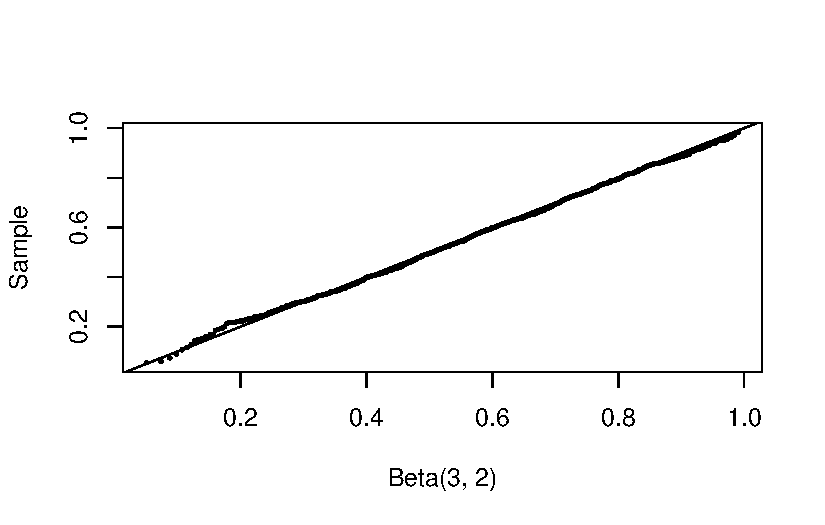
\includegraphics[keepaspectratio]{03-generating-rv_files/figure-pdf/unnamed-chunk-2-1.pdf}}

\section{Sum and Mixture}\label{sum-and-mixture}

\subsection{Sum/Convolution}\label{sumconvolution}

Let \(X_1, X_2, \ldots, X_n \overset{iid}{\sim}F_X\). Then we may
consider the sum of the random variables \(S_n:=\sum_{i=1}^n X_i\), with
distribution \(F_{S_n}\), which can be referred as \emph{convoluton}. We
can simulate \(S_n\) by simulating \(X_1, X_2, \ldots, X_n\) and summing
them up. There are several common convolutions we have seen so far

\begin{enumerate}
\def\labelenumi{\arabic{enumi}.}
\item
  Sum of \(n\) independent i.i.d. chi-square with degreee of freedom
  (df) 1 is chi-square with df \(n\).
\item
  Sum of \(n\) independent i.i.d. exponential with rate \(\lambda\) is
  gamma with shape \(n\) and rate \(\lambda\).
\item
  Sum of \(n\) independent i.i.d. geometric with parametric \(p\) is
  negative binomial with size \(n\) and parameter \(p\).
\end{enumerate}

In order to simulate \(\chi^2\) distribution with df k, we can simulate
k independent standard normal rvs and sum their squares. Let's simulate
\(n\) independent \(S \sim \chi^2(5)\).

\begin{enumerate}
\def\labelenumi{\arabic{enumi}.}
\item
  Fill an \(n \times k\) matrix with \(n k\) realization of the random
  variables that follow \(N(0,1)\).
\item
  Square each entry in the matrix (1).
\item
  Compute the row sums of the squared normals. Each row sum is one
  random observation from the \(\chi^2(k)\) distribution.
\end{enumerate}

\begin{Shaded}
\begin{Highlighting}[]
\FunctionTok{set.seed}\NormalTok{(}\DecValTok{777}\NormalTok{)}
\NormalTok{k }\OtherTok{\textless{}{-}} \DecValTok{5}
\NormalTok{n }\OtherTok{\textless{}{-}} \DecValTok{1000}
\NormalTok{X }\OtherTok{\textless{}{-}} \FunctionTok{matrix}\NormalTok{(}\FunctionTok{rnorm}\NormalTok{(n}\SpecialCharTok{*}\NormalTok{k), }\AttributeTok{nrow =}\NormalTok{ n, }\AttributeTok{ncol =}\NormalTok{ k)}\SpecialCharTok{\^{}}\DecValTok{2}
\NormalTok{X\_row }\OtherTok{\textless{}{-}} \FunctionTok{rowSums}\NormalTok{(X)}
\FunctionTok{mean}\NormalTok{(X\_row)}
\end{Highlighting}
\end{Shaded}

\begin{verbatim}
[1] 5.065355
\end{verbatim}

\begin{Shaded}
\begin{Highlighting}[]
\FunctionTok{mean}\NormalTok{(X\_row}\SpecialCharTok{\^{}}\DecValTok{2}\NormalTok{)}
\end{Highlighting}
\end{Shaded}

\begin{verbatim}
[1] 36.40181
\end{verbatim}

\subsection{Mixture}\label{mixture}

A mixture distribution is a probability distribution constructed as a
weighted sum of other distributions. If \(X\) is a rv with a mixture
distribution, then its pdf is given by \[
F_X(x) = \sum_{i=1}^k \alpha_i F_{X_i}(x),
\] where \(\alpha_i\ge 0\) and \(\sum_i \alpha_i=1\). We can just simply
simulate each \emph{component} \(X_i\) first, then multiply with their
corresponding weights \(\alpha_i\).

Suppose \(X\) and \(Y\) is a mixture of two normal distributions, where
\(X\sim N(\mu_1,\sigma_1^2)\) with probability \(\alpha\) and
\(Y\sim N(\mu_2,\sigma_2^2)\) with probability \(1-\alpha\).

\begin{Shaded}
\begin{Highlighting}[]
\NormalTok{n }\OtherTok{\textless{}{-}} \DecValTok{1000}
\NormalTok{x1 }\OtherTok{\textless{}{-}} \FunctionTok{rnorm}\NormalTok{(n, }\DecValTok{0}\NormalTok{, }\DecValTok{1}\NormalTok{)}
\NormalTok{x2 }\OtherTok{\textless{}{-}} \FunctionTok{rnorm}\NormalTok{(n, }\DecValTok{3}\NormalTok{, }\DecValTok{3}\NormalTok{)}
\NormalTok{s\_convolution }\OtherTok{\textless{}{-}}\NormalTok{ x1 }\SpecialCharTok{+}\NormalTok{ x2 }\CommentTok{\#the convolution}

\NormalTok{u }\OtherTok{\textless{}{-}} \FunctionTok{runif}\NormalTok{(n)}
\NormalTok{k }\OtherTok{\textless{}{-}} \FunctionTok{as.integer}\NormalTok{(u }\SpecialCharTok{\textgreater{}} \FloatTok{0.5}\NormalTok{) }\CommentTok{\#vector of 0’s and 1’s}

\DocumentationTok{\#\# pay attention to it}
\NormalTok{m\_mixture }\OtherTok{\textless{}{-}}\NormalTok{ k }\SpecialCharTok{*}\NormalTok{ x1 }\SpecialCharTok{+}\NormalTok{ (}\DecValTok{1}\SpecialCharTok{{-}}\NormalTok{k) }\SpecialCharTok{*}\NormalTok{ x2 }\CommentTok{\#the mixture}
\NormalTok{df }\OtherTok{\textless{}{-}} \FunctionTok{data.frame}\NormalTok{(}
  \AttributeTok{value =} \FunctionTok{c}\NormalTok{(s\_convolution, m\_mixture),}
  \AttributeTok{type =} \FunctionTok{rep}\NormalTok{(}\FunctionTok{c}\NormalTok{(}\StringTok{"convolution"}\NormalTok{, }\StringTok{"mixture"}\NormalTok{), }\AttributeTok{each =}\NormalTok{ n)}
\NormalTok{)}
\FunctionTok{ggplot}\NormalTok{(df, }\FunctionTok{aes}\NormalTok{(}\AttributeTok{x =}\NormalTok{ value, }\AttributeTok{fill =}\NormalTok{ type)) }\SpecialCharTok{+}
  \FunctionTok{geom\_histogram}\NormalTok{(}\AttributeTok{alpha =} \FloatTok{0.6}\NormalTok{, }\AttributeTok{position =} \StringTok{"identity"}\NormalTok{, }\AttributeTok{bins =} \DecValTok{40}\NormalTok{, }\AttributeTok{color =} \StringTok{"black"}\NormalTok{) }\SpecialCharTok{+}
  \FunctionTok{labs}\NormalTok{(}\AttributeTok{title =} \StringTok{"Histograms of convolution and mixture"}\NormalTok{, }\AttributeTok{x =} \StringTok{"Value"}\NormalTok{, }\AttributeTok{y =} \StringTok{"Count"}\NormalTok{) }\SpecialCharTok{+} 
  \FunctionTok{theme\_minimal}\NormalTok{()}
\end{Highlighting}
\end{Shaded}

\pandocbounded{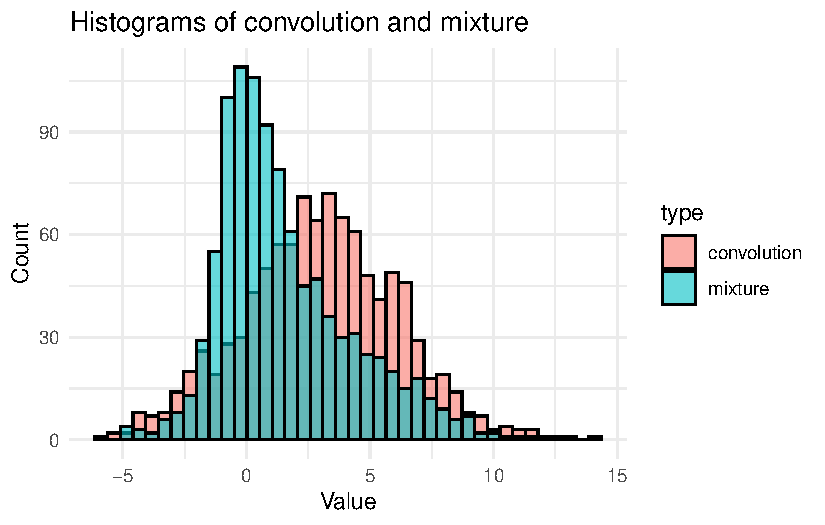
\includegraphics[keepaspectratio]{03-generating-rv_files/figure-pdf/mixture normal-1.pdf}}

\begin{tcolorbox}[enhanced jigsaw, colbacktitle=quarto-callout-note-color!10!white, coltitle=black, opacityback=0, toprule=.15mm, titlerule=0mm, breakable, bottomtitle=1mm, bottomrule=.15mm, colframe=quarto-callout-note-color-frame, leftrule=.75mm, rightrule=.15mm, arc=.35mm, title=\textcolor{quarto-callout-note-color}{\faInfo}\hspace{0.5em}{Simulate for mixture}, left=2mm, opacitybacktitle=0.6, toptitle=1mm, colback=white]

Pay attention how a mixture is simulated. In particular, we first
simulate a vector \(U\sim\operatorname{Unif}(0,1)\), then use it to
select from which distribution/component we want to sample. It is
\textbf{not an (weighted) addition} as in the convolution.

\end{tcolorbox}

\begin{tcolorbox}[enhanced jigsaw, colbacktitle=quarto-callout-note-color!10!white, coltitle=black, opacityback=0, toprule=.15mm, titlerule=0mm, breakable, bottomtitle=1mm, bottomrule=.15mm, colframe=quarto-callout-note-color-frame, leftrule=.75mm, rightrule=.15mm, arc=.35mm, title=\textcolor{quarto-callout-note-color}{\faInfo}\hspace{0.5em}{Difference between convolution and mixture}, left=2mm, opacitybacktitle=0.6, toptitle=1mm, colback=white]

Convolution is the sum of two independent rvs, while mixture is a
weighted average of two rvs. Note: Mixture is \emph{non-normal!} but the
convolution is \emph{normal}.

\end{tcolorbox}

\section{Simulate Multivaraite RVs}\label{simulate-multivaraite-rvs}

This section presents generators for the multivariate normal
distribution, multivariate normal mixtures, the Wishart distribution,
and the uniform distribution on the sphere in \(\mathbb{R}^d\).

\subsection{Multivariate normal
distribution}\label{multivariate-normal-distribution}

Recall that, from Definition 1 in Chapter 2, a \(d\)-dimensional random
vector \(X\) is a multivariate normal distribution with mean vector
\(\mu\) and covariance matrix \(\Sigma\), denoted by
\(X \sim N_d(\mu, \Sigma)\), if every linear combination of its
components has a univariate normal distribution. That is, for every
nonzero vector \(a \in \mathbb{R}^d\), the rv \(a^T X\) has a univariate
normal distribution.

To write this in an explicit form, we have, \(X = (X_1,\dots,X_N)\)
follow a multivariate normal (MVN) distribution with mean vector
\(\mu = (\mu_1,\dots,\mu_N)\) and covariance matrix
\(\Sigma = (\sigma_{ij})\), if its joint density function is given by \[
f_X(x) = \frac{1}{(2\pi)^{p/2} |\Sigma|^{1/2}} \exp\left(-\frac{1}{2}(x - \mu)^T \Sigma^{-1} (x - \mu)\right), \quad x \in \mathbb{R}^p.
\]

More explicitly, we can write this as the
\[\mu=(\mu_1,\dots,\mu_p) = \begin{pmatrix}\mu_1\\
\vdots\\
\mu_p\end{pmatrix}\in \mathbb{R}^p,\] and
\[\Sigma=(\Sigma_{ij}) = (\mathbb{C}ov(X_i,X_j))= \left[\begin{array}{cccc}
\sigma_{11} & \sigma_{12} & \ldots & \sigma_{1 d} \\
\sigma_{21} & \sigma_{22} & \ldots & \sigma_{2 d} \\
\vdots & \vdots & & \vdots \\
\sigma_{d 1} & \sigma_{d 2} & \ldots & \sigma_{d d}
\end{array}\right] \in \mathbb{R}^{d\times d}.
\]

A random vector \(X\sim N_d(\mu,\Sigma)\) can be simulated by the
following steps:

\begin{enumerate}
\def\labelenumi{\arabic{enumi}.}
\item
  Simulate \(Z = (Z_1,\ldots,Z_d)^T\) where
  \(Z_i \overset{iid}{\sim}N(0,1)\).
\item
  Find a vector \(\mu\) and a matrix \(A\) and such that
  \(\Sigma = AA^T\). The decomposition can be Cholesky decomposition,
  eigendecomposition, or singular value decomposition, etc.
\end{enumerate}

In practice, we \emph{do not do this one at a time}, we want to simulate
\(n\) sample in as few steps as possible. The following procedure is
more efficient. Typically, one applies the transformation to a data
matrix and transforms the entire sample. Suppose that
\(Z = (Z_ij ) \in \mathbb{R}^{n\times d}\), where
\(Z_{ij}\overset{iid}{\sim}N(0,1)\). Then the rows of Z are \(n\) random
observations from the \(d\)-dimensional standard MVN distribution. The
required transformation applied to the data matrix is
\[X = ZQ + J \mu^\top,\] where \(Q^\top Q=\Sigma\), and \(J\) is a
column vector of \(n\) ones. The rows of \(X\) are \(n\) random
observations from the \(d\)-dimensional MVN distribution with mean
vector \(\mu\) and covariance matrix \(\Sigma\).

Method for generating multivariate \$n \$ normal samples from the
\(N_d(\mu,\Sigma)\) distribution.

Step 1. Simulate \(Z = (Z_{ij}) \in \mathbb{R}^{n\times d}\), where
\(Z_{ij} \overset{iid}{\sim}N(0,1)\).

Step 2. Compute the decomposition \(\Sigma = Q^\top Q\).

Step 3. Compute \(X = ZQ + J\mu^\top\), where \(J\) is a column vector
of \(n\) ones.

Step 4. Return \(X\in \mathbb{R}^{ n\times d}\), in which each of the
\(n\) rows of \(X\) is a random observation from the \(N_d(\mu,\Sigma)\)
distribution.

\subsubsection{A few things to be
considered}\label{a-few-things-to-be-considered}

\begin{enumerate}
\def\labelenumi{\arabic{enumi}.}
\tightlist
\item
  Computation of \(J \mu^\top\)
\end{enumerate}

Recall that \(J\) is a vector of 1's (i.e.,
\(J=(1,\dots,1)\in\mathbb{R}^d\) and \(\mu^\top\) is the transpose of
\(\mu\). So, \(J \mu^\top\) is a matrix with each row being \(\mu\). In
R, we can use \texttt{matrix(mu,\ n,\ d,\ byrow\ =\ TRUE)} to create
this matrix. Also, for any \(i\) and \(j\), \(\mu_i=\mu_j=c\), where c
is a constant, then we can write it as \(c I_{n\times d}\), where
\(I_{n\times d}\) is a matrix of 1's with dimension \(n\times d\).

\begin{Shaded}
\begin{Highlighting}[]
\NormalTok{Z }\OtherTok{\textless{}{-}} \FunctionTok{matrix}\NormalTok{(}\FunctionTok{rnorm}\NormalTok{(n}\SpecialCharTok{*}\NormalTok{d), }\AttributeTok{nrow =}\NormalTok{ n, }\AttributeTok{ncol =}\NormalTok{ d)}
\NormalTok{X }\OtherTok{\textless{}{-}}\NormalTok{ Z }\SpecialCharTok{\%*\%}\NormalTok{ Q }\SpecialCharTok{+} \FunctionTok{matrix}\NormalTok{(mu, n, d, }\AttributeTok{byrow =} \ConstantTok{TRUE}\NormalTok{)}
\end{Highlighting}
\end{Shaded}

\begin{enumerate}
\def\labelenumi{\arabic{enumi}.}
\setcounter{enumi}{1}
\tightlist
\item
  Decomposition of \(\Sigma\)
\end{enumerate}

There are many different ways to decompose \(\Sigma\). Recall that
\(\Sigma\) is a symmetric positive definite matrix, so we can use
Cholesky decomposition, eigendecomposition, or singular value
decomposition (SVD). In R, we can use \texttt{chol()}, \texttt{eigen()},
or \texttt{svd()} functions to compute the decomposition.

\begin{itemize}
\item
  \textbf{Choleski decomposition}: Choleski of a real symmetric
  positive-definite matrix is \(X = Q^\top Q\), where \(Q\) is an upper
  triangular matrix.
\item
  \textbf{Spectral decomposition}: The square root of the covariance is
  \(Σ^{1/2} = P^{1/2} \Lambda P^{−1}\), where \(\Lambda\) is the
  diagonal matrix with the eigenvalues of \(\Sigma\) along the diagonal
  and \(P\) is the matrix whose columns are the eigenvectors of
  \(\Sigma\) corresponding to the eigenvalues in \(\Lambda\). This
  method can also be called the eigen-decomposition method. In the
  eigen-decomposition we have \(P^{-1}= P^\top\) and therefore
  \(Σ^{1/2} = P \Lambda^{1/2}P^\top\) . The matrix \(Q = Σ^{1/2}\) is a
  factorization of \(\Sigma\) such that \(Q^\top Q = \Sigma\).
\item
  \textbf{Singular Value Decomposition}: The singular value
  decomposition (svd) generalizes the idea of eigenvectors to
  rectangular matrices. The svd of a matrix \(X\) is \(X = U DV^\top\) ,
  where D is a vector containing the singular values of \(X\), \(U\) is
  a matrix whose columns contain the left singular vectors of \(X\), and
  \(V\) is a matrix whose columns contain the right singular vectors of
  \(X\). The matrix \(X\) in this case is the population covariance
  matrix \(\Sigma\), and \(UV\top = I\). The svd of a symmetric positive
  definite matrix \(\Sigma\) gives \(U = V = P\) and
  \(Σ^{1/2} = U D^{1/2}V^\top\) . Thus the svd method for this
  application is equivalent to the spectral decomposition method, but is
  \textbf{less efficient} because the svd method does not take advantage
  of the fact that the matrix \(\Sigma\) is square symmetric.
\end{itemize}

\begin{tcolorbox}[enhanced jigsaw, colbacktitle=quarto-callout-note-color!10!white, coltitle=black, opacityback=0, toprule=.15mm, titlerule=0mm, breakable, bottomtitle=1mm, bottomrule=.15mm, colframe=quarto-callout-note-color-frame, leftrule=.75mm, rightrule=.15mm, arc=.35mm, title=\textcolor{quarto-callout-note-color}{\faInfo}\hspace{0.5em}{Performance Comparison}, left=2mm, opacitybacktitle=0.6, toptitle=1mm, colback=white]

\begin{Shaded}
\begin{Highlighting}[]
\FunctionTok{set.seed}\NormalTok{(}\DecValTok{777}\NormalTok{)}


\NormalTok{n  }\OtherTok{\textless{}{-}} \DecValTok{100}     \CommentTok{\# sample size per call}
\NormalTok{d  }\OtherTok{\textless{}{-}} \DecValTok{30}      \CommentTok{\# dimension}
\NormalTok{N  }\OtherTok{\textless{}{-}} \DecValTok{1000}    \CommentTok{\# number of distinct Sigmas to cycle through in Scenario A}
\NormalTok{reps\_A }\OtherTok{\textless{}{-}} \DecValTok{200} \CommentTok{\# microbenchmark repetitions for Scenario A}
\NormalTok{reps\_B }\OtherTok{\textless{}{-}} \DecValTok{500} \CommentTok{\# microbenchmark repetitions for Scenario B}
\NormalTok{mu }\OtherTok{\textless{}{-}} \FunctionTok{numeric}\NormalTok{(d)}

\DocumentationTok{\#\# ====== MVN generators ======}
\NormalTok{rmvn\_eigen }\OtherTok{\textless{}{-}} \ControlFlowTok{function}\NormalTok{(n, mu, Sigma) \{}
\NormalTok{  ev }\OtherTok{\textless{}{-}} \FunctionTok{eigen}\NormalTok{(Sigma, }\AttributeTok{symmetric =} \ConstantTok{TRUE}\NormalTok{)}
\NormalTok{  A  }\OtherTok{\textless{}{-}}\NormalTok{ ev}\SpecialCharTok{$}\NormalTok{vectors }\SpecialCharTok{\%*\%}\NormalTok{ (}\FunctionTok{sqrt}\NormalTok{(}\FunctionTok{pmax}\NormalTok{(ev}\SpecialCharTok{$}\NormalTok{values, }\DecValTok{0}\NormalTok{)) }\SpecialCharTok{*} \FunctionTok{t}\NormalTok{(ev}\SpecialCharTok{$}\NormalTok{vectors))}
\NormalTok{  Z  }\OtherTok{\textless{}{-}} \FunctionTok{matrix}\NormalTok{(}\FunctionTok{rnorm}\NormalTok{(n }\SpecialCharTok{*} \FunctionTok{length}\NormalTok{(mu)), n)}
  \FunctionTok{sweep}\NormalTok{(Z }\SpecialCharTok{\%*\%}\NormalTok{ A, }\DecValTok{2}\NormalTok{, mu, }\StringTok{\textasciigrave{}}\AttributeTok{+}\StringTok{\textasciigrave{}}\NormalTok{)}
\NormalTok{\}}

\NormalTok{rmvn\_svd }\OtherTok{\textless{}{-}} \ControlFlowTok{function}\NormalTok{(n, mu, Sigma) \{}
\NormalTok{  sv }\OtherTok{\textless{}{-}} \FunctionTok{svd}\NormalTok{(Sigma)}
\NormalTok{  A  }\OtherTok{\textless{}{-}}\NormalTok{ sv}\SpecialCharTok{$}\NormalTok{u }\SpecialCharTok{\%*\%}\NormalTok{ (}\FunctionTok{sqrt}\NormalTok{(}\FunctionTok{pmax}\NormalTok{(sv}\SpecialCharTok{$}\NormalTok{d, }\DecValTok{0}\NormalTok{)) }\SpecialCharTok{*} \FunctionTok{t}\NormalTok{(sv}\SpecialCharTok{$}\NormalTok{v))}
\NormalTok{  Z  }\OtherTok{\textless{}{-}} \FunctionTok{matrix}\NormalTok{(}\FunctionTok{rnorm}\NormalTok{(n }\SpecialCharTok{*} \FunctionTok{length}\NormalTok{(mu)), n)}
  \FunctionTok{sweep}\NormalTok{(Z }\SpecialCharTok{\%*\%}\NormalTok{ A, }\DecValTok{2}\NormalTok{, mu, }\StringTok{\textasciigrave{}}\AttributeTok{+}\StringTok{\textasciigrave{}}\NormalTok{)}
\NormalTok{\}}

\NormalTok{rmvn\_chol }\OtherTok{\textless{}{-}} \ControlFlowTok{function}\NormalTok{(n, mu, Sigma) \{}
\NormalTok{  R  }\OtherTok{\textless{}{-}} \FunctionTok{chol}\NormalTok{(Sigma)}
\NormalTok{  Z  }\OtherTok{\textless{}{-}} \FunctionTok{matrix}\NormalTok{(}\FunctionTok{rnorm}\NormalTok{(n }\SpecialCharTok{*} \FunctionTok{length}\NormalTok{(mu)), n)}
  \FunctionTok{sweep}\NormalTok{(Z }\SpecialCharTok{\%*\%}\NormalTok{ R, }\DecValTok{2}\NormalTok{, mu, }\StringTok{\textasciigrave{}}\AttributeTok{+}\StringTok{\textasciigrave{}}\NormalTok{)}
\NormalTok{\}}

\DocumentationTok{\#\# ====== Utilities ======}
\NormalTok{rand\_cov }\OtherTok{\textless{}{-}} \ControlFlowTok{function}\NormalTok{(d) \{}
\NormalTok{  A }\OtherTok{\textless{}{-}} \FunctionTok{matrix}\NormalTok{(}\FunctionTok{rnorm}\NormalTok{(d}\SpecialCharTok{*}\NormalTok{d), d, d)}
\NormalTok{  S }\OtherTok{\textless{}{-}} \FunctionTok{crossprod}\NormalTok{(A) }\SpecialCharTok{/}\NormalTok{ d}
  \FunctionTok{diag}\NormalTok{(S) }\OtherTok{\textless{}{-}} \FunctionTok{diag}\NormalTok{(S) }\SpecialCharTok{+} \FloatTok{1e{-}6}
\NormalTok{  S}
\NormalTok{\}}

\NormalTok{drop\_outliers }\OtherTok{\textless{}{-}} \ControlFlowTok{function}\NormalTok{(df) \{}
\NormalTok{  df }\SpecialCharTok{\%\textgreater{}\%}
    \FunctionTok{group\_by}\NormalTok{(expr) }\SpecialCharTok{\%\textgreater{}\%}
    \FunctionTok{mutate}\NormalTok{(}
      \AttributeTok{q1 =} \FunctionTok{quantile}\NormalTok{(time, }\FloatTok{0.25}\NormalTok{),}
      \AttributeTok{q3 =} \FunctionTok{quantile}\NormalTok{(time, }\FloatTok{0.75}\NormalTok{),}
      \AttributeTok{iqr =}\NormalTok{ q3 }\SpecialCharTok{{-}}\NormalTok{ q1,}
      \AttributeTok{lower =}\NormalTok{ q1 }\SpecialCharTok{{-}} \FloatTok{1.5} \SpecialCharTok{*}\NormalTok{ iqr,}
      \AttributeTok{upper =}\NormalTok{ q3 }\SpecialCharTok{+} \FloatTok{1.5} \SpecialCharTok{*}\NormalTok{ iqr}
\NormalTok{    ) }\SpecialCharTok{\%\textgreater{}\%}
    \FunctionTok{filter}\NormalTok{(time }\SpecialCharTok{\textgreater{}=}\NormalTok{ lower }\SpecialCharTok{\&}\NormalTok{ time }\SpecialCharTok{\textless{}=}\NormalTok{ upper) }\SpecialCharTok{\%\textgreater{}\%}
    \FunctionTok{ungroup}\NormalTok{()}
\NormalTok{\}}

\DocumentationTok{\#\# Precompute N random SPD matrices (same pool for all methods)}
\NormalTok{Sigma\_list }\OtherTok{\textless{}{-}} \FunctionTok{replicate}\NormalTok{(N, }\FunctionTok{rand\_cov}\NormalTok{(d), }\AttributeTok{simplify =} \ConstantTok{FALSE}\NormalTok{)}

\DocumentationTok{\#\# ====== Scenario A: varying Sigma each call (factorize every time) ======}
\NormalTok{i }\OtherTok{\textless{}{-}} \DecValTok{0}
\NormalTok{next\_Sigma }\OtherTok{\textless{}{-}} \ControlFlowTok{function}\NormalTok{() \{ i }\OtherTok{\textless{}\textless{}{-}} \ControlFlowTok{if}\NormalTok{ (i }\SpecialCharTok{==}\NormalTok{ N) }\DecValTok{1} \ControlFlowTok{else}\NormalTok{ i }\SpecialCharTok{+} \DecValTok{1}\NormalTok{; Sigma\_list[[i]] \}}

\NormalTok{bench\_A }\OtherTok{\textless{}{-}} \FunctionTok{microbenchmark}\NormalTok{(}
  \AttributeTok{rmvn\_eigen       =} \FunctionTok{rmvn\_eigen}\NormalTok{(n, mu, }\FunctionTok{next\_Sigma}\NormalTok{()),}
  \AttributeTok{rmvn\_svd         =} \FunctionTok{rmvn\_svd}\NormalTok{(n,   mu, }\FunctionTok{next\_Sigma}\NormalTok{()),}
  \AttributeTok{rmvn\_chol        =} \FunctionTok{rmvn\_chol}\NormalTok{(n,  mu, }\FunctionTok{next\_Sigma}\NormalTok{()),}
  \AttributeTok{MASS\_mvrnorm     =}\NormalTok{ MASS}\SpecialCharTok{::}\FunctionTok{mvrnorm}\NormalTok{(n, mu, }\FunctionTok{next\_Sigma}\NormalTok{()),}
  \AttributeTok{mvtnorm\_rmvnorm  =}\NormalTok{ mvtnorm}\SpecialCharTok{::}\FunctionTok{rmvnorm}\NormalTok{(n, }\AttributeTok{mean =}\NormalTok{ mu, }\AttributeTok{sigma =} \FunctionTok{next\_Sigma}\NormalTok{()),}
  \AttributeTok{times =}\NormalTok{ reps\_A}
\NormalTok{)}

\NormalTok{sum\_A }\OtherTok{\textless{}{-}} \FunctionTok{as.data.frame}\NormalTok{(bench\_A) }\SpecialCharTok{\%\textgreater{}\%}
  \FunctionTok{group\_by}\NormalTok{(expr) }\SpecialCharTok{\%\textgreater{}\%}
  \FunctionTok{summarize}\NormalTok{(}\AttributeTok{median\_ms =} \FunctionTok{median}\NormalTok{(time)}\SpecialCharTok{/}\FloatTok{1e6}\NormalTok{,}
            \AttributeTok{iqr\_ms    =} \FunctionTok{IQR}\NormalTok{(time)}\SpecialCharTok{/}\FloatTok{1e6}\NormalTok{,}
            \AttributeTok{.groups =} \StringTok{"drop"}\NormalTok{) }\SpecialCharTok{\%\textgreater{}\%}
  \FunctionTok{arrange}\NormalTok{(median\_ms) }\SpecialCharTok{\%\textgreater{}\%}
  \FunctionTok{mutate}\NormalTok{(}\AttributeTok{scenario =} \StringTok{"A: varying Σ"}\NormalTok{)}

\FunctionTok{print}\NormalTok{(sum\_A)}
\end{Highlighting}
\end{Shaded}

\begin{verbatim}
# A tibble: 5 x 4
  expr            median_ms  iqr_ms scenario    
  <fct>               <dbl>   <dbl> <chr>       
1 rmvn_chol           0.129 0.00861 A: varying Σ
2 MASS_mvrnorm        0.196 0.0106  A: varying Σ
3 rmvn_eigen          0.201 0.0123  A: varying Σ
4 rmvn_svd            0.246 0.0181  A: varying Σ
5 mvtnorm_rmvnorm     0.266 0.0244  A: varying Σ
\end{verbatim}

\begin{Shaded}
\begin{Highlighting}[]
\NormalTok{pA }\OtherTok{\textless{}{-}} \FunctionTok{drop\_outliers}\NormalTok{(}\FunctionTok{as.data.frame}\NormalTok{(bench\_A)) }\SpecialCharTok{\%\textgreater{}\%}
  \FunctionTok{mutate}\NormalTok{(}\AttributeTok{ms =}\NormalTok{ time}\SpecialCharTok{/}\FloatTok{1e6}\NormalTok{) }\SpecialCharTok{\%\textgreater{}\%}
  \FunctionTok{ggplot}\NormalTok{(}\FunctionTok{aes}\NormalTok{(}\AttributeTok{x =} \FunctionTok{reorder}\NormalTok{(expr, ms, }\AttributeTok{FUN =}\NormalTok{ median), }\AttributeTok{y =}\NormalTok{ ms)) }\SpecialCharTok{+}
  \FunctionTok{geom\_boxplot}\NormalTok{() }\SpecialCharTok{+}
  \FunctionTok{stat\_summary}\NormalTok{(}\AttributeTok{fun =}\NormalTok{ median, }\AttributeTok{geom =} \StringTok{"point"}\NormalTok{, }\AttributeTok{shape =} \DecValTok{21}\NormalTok{, }\AttributeTok{size =} \DecValTok{2}\NormalTok{, }\AttributeTok{stroke =} \FloatTok{0.6}\NormalTok{) }\SpecialCharTok{+}
  \FunctionTok{coord\_flip}\NormalTok{() }\SpecialCharTok{+}
  \FunctionTok{labs}\NormalTok{(}\AttributeTok{title =} \StringTok{"MVN generators — Scenario A (varying Σ, outliers removed)"}\NormalTok{,}
       \AttributeTok{x =} \ConstantTok{NULL}\NormalTok{, }\AttributeTok{y =} \StringTok{"Time (ms) per call)"}\NormalTok{) }\SpecialCharTok{+}
  \FunctionTok{theme\_minimal}\NormalTok{(}\AttributeTok{base\_size =} \DecValTok{12}\NormalTok{)}

\FunctionTok{print}\NormalTok{(pA)}
\end{Highlighting}
\end{Shaded}

\pandocbounded{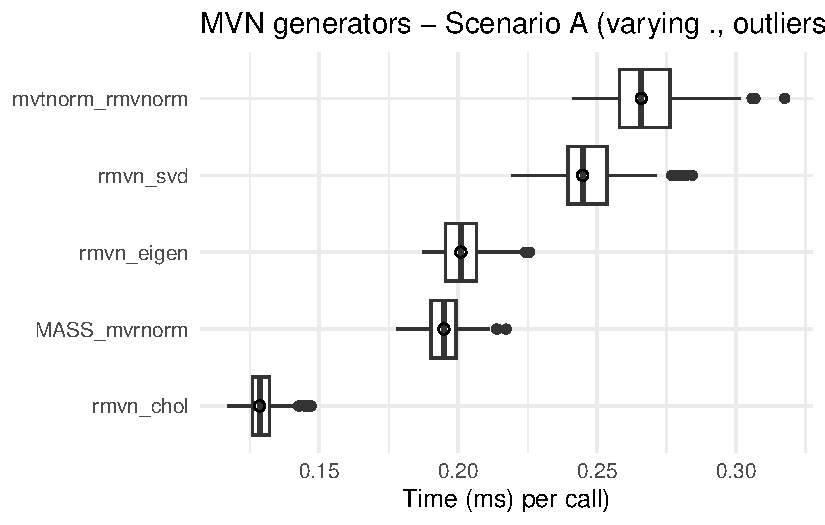
\includegraphics[keepaspectratio]{03-generating-rv_files/figure-pdf/MVM-performance-1.pdf}}

\begin{Shaded}
\begin{Highlighting}[]
\DocumentationTok{\#\# ====== Scenario B: fixed Sigma, reuse factorization when possible ======}
\NormalTok{Sigma0 }\OtherTok{\textless{}{-}}\NormalTok{ Sigma\_list[[}\DecValTok{1}\NormalTok{]]}

\NormalTok{rmvn\_chol\_fixed }\OtherTok{\textless{}{-}} \FunctionTok{local}\NormalTok{(\{}
\NormalTok{  R }\OtherTok{\textless{}{-}} \FunctionTok{chol}\NormalTok{(Sigma0)}
  \ControlFlowTok{function}\NormalTok{(n, mu) \{}
\NormalTok{    Z }\OtherTok{\textless{}{-}} \FunctionTok{matrix}\NormalTok{(}\FunctionTok{rnorm}\NormalTok{(n }\SpecialCharTok{*} \FunctionTok{length}\NormalTok{(mu)), n)}
    \FunctionTok{sweep}\NormalTok{(Z }\SpecialCharTok{\%*\%}\NormalTok{ R, }\DecValTok{2}\NormalTok{, mu, }\StringTok{\textasciigrave{}}\AttributeTok{+}\StringTok{\textasciigrave{}}\NormalTok{)}
\NormalTok{  \}}
\NormalTok{\})}

\NormalTok{rmvn\_eigen\_fixed }\OtherTok{\textless{}{-}} \FunctionTok{local}\NormalTok{(\{}
\NormalTok{  ev }\OtherTok{\textless{}{-}} \FunctionTok{eigen}\NormalTok{(Sigma0, }\AttributeTok{symmetric =} \ConstantTok{TRUE}\NormalTok{)}
\NormalTok{  A  }\OtherTok{\textless{}{-}}\NormalTok{ ev}\SpecialCharTok{$}\NormalTok{vectors }\SpecialCharTok{\%*\%}\NormalTok{ (}\FunctionTok{sqrt}\NormalTok{(}\FunctionTok{pmax}\NormalTok{(ev}\SpecialCharTok{$}\NormalTok{values, }\DecValTok{0}\NormalTok{)) }\SpecialCharTok{*} \FunctionTok{t}\NormalTok{(ev}\SpecialCharTok{$}\NormalTok{vectors))}
  \ControlFlowTok{function}\NormalTok{(n, mu) \{}
\NormalTok{    Z }\OtherTok{\textless{}{-}} \FunctionTok{matrix}\NormalTok{(}\FunctionTok{rnorm}\NormalTok{(n }\SpecialCharTok{*} \FunctionTok{length}\NormalTok{(mu)), n)}
    \FunctionTok{sweep}\NormalTok{(Z }\SpecialCharTok{\%*\%}\NormalTok{ A, }\DecValTok{2}\NormalTok{, mu, }\StringTok{\textasciigrave{}}\AttributeTok{+}\StringTok{\textasciigrave{}}\NormalTok{)}
\NormalTok{  \}}
\NormalTok{\})}

\NormalTok{rmvn\_svd\_fixed }\OtherTok{\textless{}{-}} \FunctionTok{local}\NormalTok{(\{}
\NormalTok{  sv }\OtherTok{\textless{}{-}} \FunctionTok{svd}\NormalTok{(Sigma0)}
\NormalTok{  A  }\OtherTok{\textless{}{-}}\NormalTok{ sv}\SpecialCharTok{$}\NormalTok{u }\SpecialCharTok{\%*\%}\NormalTok{ (}\FunctionTok{sqrt}\NormalTok{(}\FunctionTok{pmax}\NormalTok{(sv}\SpecialCharTok{$}\NormalTok{d, }\DecValTok{0}\NormalTok{)) }\SpecialCharTok{*} \FunctionTok{t}\NormalTok{(sv}\SpecialCharTok{$}\NormalTok{v))}
  \ControlFlowTok{function}\NormalTok{(n, mu) \{}
\NormalTok{    Z }\OtherTok{\textless{}{-}} \FunctionTok{matrix}\NormalTok{(}\FunctionTok{rnorm}\NormalTok{(n }\SpecialCharTok{*} \FunctionTok{length}\NormalTok{(mu)), n)}
    \FunctionTok{sweep}\NormalTok{(Z }\SpecialCharTok{\%*\%}\NormalTok{ A, }\DecValTok{2}\NormalTok{, mu, }\StringTok{\textasciigrave{}}\AttributeTok{+}\StringTok{\textasciigrave{}}\NormalTok{)}
\NormalTok{  \}}
\NormalTok{\})}

\NormalTok{bench\_B }\OtherTok{\textless{}{-}} \FunctionTok{microbenchmark}\NormalTok{(}
  \AttributeTok{rmvn\_chol\_fixed   =} \FunctionTok{rmvn\_chol\_fixed}\NormalTok{(n, mu),}
  \AttributeTok{rmvn\_eigen\_fixed  =} \FunctionTok{rmvn\_eigen\_fixed}\NormalTok{(n, mu),}
  \AttributeTok{rmvn\_svd\_fixed    =} \FunctionTok{rmvn\_svd\_fixed}\NormalTok{(n, mu),}
  \AttributeTok{MASS\_mvrnorm      =}\NormalTok{ MASS}\SpecialCharTok{::}\FunctionTok{mvrnorm}\NormalTok{(n, mu, Sigma0),                   }\CommentTok{\# factorizes internally}
  \AttributeTok{mvtnorm\_rmvnorm   =}\NormalTok{ mvtnorm}\SpecialCharTok{::}\FunctionTok{rmvnorm}\NormalTok{(n, }\AttributeTok{mean =}\NormalTok{ mu, }\AttributeTok{sigma =}\NormalTok{ Sigma0), }\CommentTok{\# Cholesky internally}
  \AttributeTok{times =}\NormalTok{ reps\_B}
\NormalTok{)}

\NormalTok{sum\_B }\OtherTok{\textless{}{-}} \FunctionTok{as.data.frame}\NormalTok{(bench\_B) }\SpecialCharTok{\%\textgreater{}\%}
  \FunctionTok{group\_by}\NormalTok{(expr) }\SpecialCharTok{\%\textgreater{}\%}
  \FunctionTok{summarize}\NormalTok{(}\AttributeTok{median\_ms =} \FunctionTok{median}\NormalTok{(time)}\SpecialCharTok{/}\FloatTok{1e6}\NormalTok{,}
            \AttributeTok{iqr\_ms    =} \FunctionTok{IQR}\NormalTok{(time)}\SpecialCharTok{/}\FloatTok{1e6}\NormalTok{,}
            \AttributeTok{.groups =} \StringTok{"drop"}\NormalTok{) }\SpecialCharTok{\%\textgreater{}\%}
  \FunctionTok{arrange}\NormalTok{(median\_ms) }\SpecialCharTok{\%\textgreater{}\%}
  \FunctionTok{mutate}\NormalTok{(}\AttributeTok{scenario =} \StringTok{"B: fixed Σ"}\NormalTok{)}

\FunctionTok{print}\NormalTok{(sum\_B)}
\end{Highlighting}
\end{Shaded}

\begin{verbatim}
# A tibble: 5 x 4
  expr             median_ms  iqr_ms scenario  
  <fct>                <dbl>   <dbl> <chr>     
1 rmvn_chol_fixed      0.119 0.00833 B: fixed Σ
2 rmvn_eigen_fixed     0.119 0.00857 B: fixed Σ
3 rmvn_svd_fixed       0.119 0.00805 B: fixed Σ
4 MASS_mvrnorm         0.185 0.0132  B: fixed Σ
5 mvtnorm_rmvnorm      0.251 0.0194  B: fixed Σ
\end{verbatim}

\begin{Shaded}
\begin{Highlighting}[]
\NormalTok{pB }\OtherTok{\textless{}{-}} \FunctionTok{drop\_outliers}\NormalTok{(}\FunctionTok{as.data.frame}\NormalTok{(bench\_B)) }\SpecialCharTok{\%\textgreater{}\%}
  \FunctionTok{mutate}\NormalTok{(}\AttributeTok{ms =}\NormalTok{ time}\SpecialCharTok{/}\FloatTok{1e6}\NormalTok{) }\SpecialCharTok{\%\textgreater{}\%}
  \FunctionTok{ggplot}\NormalTok{(}\FunctionTok{aes}\NormalTok{(}\AttributeTok{x =} \FunctionTok{reorder}\NormalTok{(expr, ms, }\AttributeTok{FUN =}\NormalTok{ median), }\AttributeTok{y =}\NormalTok{ ms)) }\SpecialCharTok{+}
  \FunctionTok{geom\_boxplot}\NormalTok{() }\SpecialCharTok{+}
  \FunctionTok{stat\_summary}\NormalTok{(}\AttributeTok{fun =}\NormalTok{ median, }\AttributeTok{geom =} \StringTok{"point"}\NormalTok{, }\AttributeTok{shape =} \DecValTok{21}\NormalTok{, }\AttributeTok{size =} \DecValTok{2}\NormalTok{, }\AttributeTok{stroke =} \FloatTok{0.6}\NormalTok{) }\SpecialCharTok{+}
  \FunctionTok{coord\_flip}\NormalTok{() }\SpecialCharTok{+}
  \FunctionTok{labs}\NormalTok{(}\AttributeTok{title =} \StringTok{"MVN generators — Scenario B (fixed Σ; outliers removed)"}\NormalTok{,}
       \AttributeTok{x =} \ConstantTok{NULL}\NormalTok{, }\AttributeTok{y =} \StringTok{"Time (ms) per call)"}\NormalTok{) }\SpecialCharTok{+}
  \FunctionTok{theme\_minimal}\NormalTok{(}\AttributeTok{base\_size =} \DecValTok{12}\NormalTok{)}

\FunctionTok{print}\NormalTok{(pB)}
\end{Highlighting}
\end{Shaded}

\pandocbounded{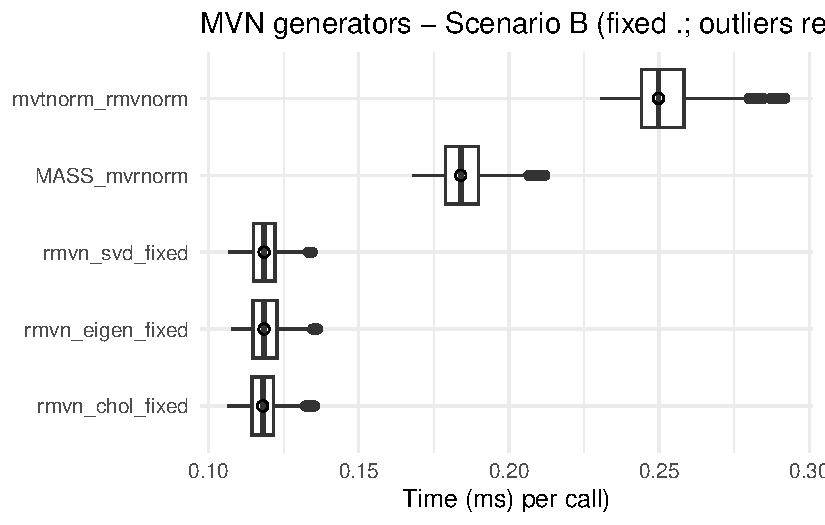
\includegraphics[keepaspectratio]{03-generating-rv_files/figure-pdf/MVM-performance-2.pdf}}

\end{tcolorbox}

\subsection{Mixture of Multivariate
Normal}\label{mixture-of-multivariate-normal}

A mixture of multivariate normal distributions is a convex combination
of multivariate normal distributions. That is, the density function of a
mixture of \(k\) multivariate normal distributions is given by \[
\alpha N_p(\mu_1,\Sigma_1) + (1-\alpha) N_p(\mu_2,\Sigma_2), \quad 0 < \alpha < 1.
\] Similar to the univariate case, different choice of \(\alpha\) will
lead to different degree of departure from the normal.

Given a \(\alpha\), to simulatecallout-note a random sample from
\(\alpha N_d(\mu_1, \Sigma_1) + (1 − p) N_d(\mu_2, \Sigma_2)\)

There are two ways.

Way 1:

\begin{enumerate}
\def\labelenumi{\arabic{enumi}.}
\item
  Generate \(U \sim unif(0,1) \in \mathbb{R}^n\).
\item
  (Component-wise) If \(U_i \le \alpha\), generate X from
  \(X_i\sim N_d(\mu_1, \Sigma_1)\), o.w. generate
  \(X_i from \sim N_d(\mu_2, \Sigma_2)\).
\end{enumerate}

Equivalent:

Way 2:

\begin{enumerate}
\def\labelenumi{\arabic{enumi}.}
\item
  Generate \(N \sim ∼ \operatorname{Bern}(\alpha)\).
\item
  (Component-wise) If \(N_i = 1\) generate \(X\) from
  \(X_i \sim N_d(\mu_1, \Sigma_1)\), o.w. generate \(X\) from
  \(N_d(\mu_2, \Sigma_2)\).
\end{enumerate}

\begin{Shaded}
\begin{Highlighting}[]
\FunctionTok{set.seed}\NormalTok{(}\DecValTok{777}\NormalTok{)}
\NormalTok{loc.mix}\FloatTok{.0} \OtherTok{\textless{}{-}} \ControlFlowTok{function}\NormalTok{(n, alpha, mu1, mu2, Sigma) \{}
  \CommentTok{\# generate sample from BVN location mixture}
\NormalTok{  X }\OtherTok{\textless{}{-}} \FunctionTok{matrix}\NormalTok{(}\DecValTok{0}\NormalTok{, n, }\DecValTok{2}\NormalTok{)}
  \ControlFlowTok{for}\NormalTok{ (i }\ControlFlowTok{in} \DecValTok{1}\SpecialCharTok{:}\NormalTok{n) \{}
\NormalTok{    k }\OtherTok{\textless{}{-}} \FunctionTok{rbinom}\NormalTok{(}\DecValTok{1}\NormalTok{, }\AttributeTok{size =} \DecValTok{1}\NormalTok{, }\AttributeTok{prob =}\NormalTok{ alpha)}
    \ControlFlowTok{if}\NormalTok{ (k) \{}
\NormalTok{      X[i, ] }\OtherTok{\textless{}{-}} \FunctionTok{mvrnorm}\NormalTok{(}\DecValTok{1}\NormalTok{, }\AttributeTok{mu =}\NormalTok{ mu1, Sigma)}
\NormalTok{    \} }\ControlFlowTok{else}\NormalTok{ \{}
\NormalTok{      X[i, ] }\OtherTok{\textless{}{-}} \FunctionTok{mvrnorm}\NormalTok{(}\DecValTok{1}\NormalTok{, }\AttributeTok{mu =}\NormalTok{ mu2, Sigma)}
\NormalTok{    \}}
\NormalTok{  \}}
  \FunctionTok{return}\NormalTok{(X)}
\NormalTok{\}}
\end{Highlighting}
\end{Shaded}

\begin{Shaded}
\begin{Highlighting}[]
\NormalTok{loc.mix }\OtherTok{\textless{}{-}} \ControlFlowTok{function}\NormalTok{(n, alpha, mu1, mu2, Sigma) \{}
  \CommentTok{\# generate sample from BVN location mixture}
\NormalTok{  n1 }\OtherTok{\textless{}{-}} \FunctionTok{rbinom}\NormalTok{(}\DecValTok{1}\NormalTok{, }\AttributeTok{size =}\NormalTok{ n, }\AttributeTok{prob =}\NormalTok{ alpha)}
\NormalTok{  n2 }\OtherTok{\textless{}{-}}\NormalTok{ n }\SpecialCharTok{{-}}\NormalTok{ n1}
\NormalTok{  x1 }\OtherTok{\textless{}{-}} \FunctionTok{mvrnorm}\NormalTok{(n1, }\AttributeTok{mu =}\NormalTok{ mu1, Sigma)}
\NormalTok{  x2 }\OtherTok{\textless{}{-}} \FunctionTok{mvrnorm}\NormalTok{(n2, }\AttributeTok{mu =}\NormalTok{ mu2, Sigma)}
\NormalTok{  X }\OtherTok{\textless{}{-}} \FunctionTok{rbind}\NormalTok{(x1, x2) }\CommentTok{\# combine the samples}
  \FunctionTok{return}\NormalTok{(X[}\FunctionTok{sample}\NormalTok{(}\DecValTok{1}\SpecialCharTok{:}\NormalTok{n), ]) }\CommentTok{\# mix them}
\NormalTok{\}}
\end{Highlighting}
\end{Shaded}

\begin{tcolorbox}[enhanced jigsaw, colbacktitle=quarto-callout-note-color!10!white, coltitle=black, opacityback=0, toprule=.15mm, titlerule=0mm, breakable, bottomtitle=1mm, bottomrule=.15mm, colframe=quarto-callout-note-color-frame, leftrule=.75mm, rightrule=.15mm, arc=.35mm, title=\textcolor{quarto-callout-note-color}{\faInfo}\hspace{0.5em}{Mixture of multivariate normal}, left=2mm, opacitybacktitle=0.6, toptitle=1mm, colback=white]

One interesting example is when
\(\alpha = 1 − 1/2 (1 − \sqrt{3}/3 )\approx .
0.7887\), provides an example of a skewed distribution with normal
kurtosis (level of the peak).

\begin{Shaded}
\begin{Highlighting}[]
\FunctionTok{set.seed}\NormalTok{(}\DecValTok{777}\NormalTok{)}


\NormalTok{n }\OtherTok{\textless{}{-}} \DecValTok{1000}
\NormalTok{comp1 }\OtherTok{\textless{}{-}}\NormalTok{ MASS}\SpecialCharTok{::}\FunctionTok{mvrnorm}\NormalTok{(n, }\AttributeTok{mu =} \FunctionTok{c}\NormalTok{(}\DecValTok{0}\NormalTok{, }\DecValTok{0}\NormalTok{), }\AttributeTok{Sigma =} \FunctionTok{diag}\NormalTok{(}\DecValTok{2}\NormalTok{))}
\NormalTok{comp2 }\OtherTok{\textless{}{-}}\NormalTok{ MASS}\SpecialCharTok{::}\FunctionTok{mvrnorm}\NormalTok{(n, }\AttributeTok{mu =} \FunctionTok{c}\NormalTok{(}\DecValTok{3}\NormalTok{, }\DecValTok{2}\NormalTok{), }\AttributeTok{Sigma =} \FunctionTok{matrix}\NormalTok{(}\FunctionTok{c}\NormalTok{(}\DecValTok{1}\NormalTok{, }\FloatTok{0.5}\NormalTok{, }\FloatTok{0.5}\NormalTok{, }\DecValTok{1}\NormalTok{), }\DecValTok{2}\NormalTok{))}

\CommentTok{\# Proper mixture membership per observation}
\NormalTok{alpha }\OtherTok{\textless{}{-}} \DecValTok{1} \SpecialCharTok{{-}} \DecValTok{1}\SpecialCharTok{/}\DecValTok{2}\SpecialCharTok{*}\NormalTok{(}\DecValTok{1} \SpecialCharTok{{-}} \FunctionTok{sqrt}\NormalTok{(}\DecValTok{3}\NormalTok{)}\SpecialCharTok{/}\DecValTok{3}\NormalTok{ )   }\CommentTok{\# P(Comp1)}
\NormalTok{memb }\OtherTok{\textless{}{-}} \FunctionTok{rbinom}\NormalTok{(n, }\DecValTok{1}\NormalTok{, alpha)         }\CommentTok{\# 1 = Comp1, 0 = Comp2}

\CommentTok{\# Build the mixture matrix row{-}wise (avoid ifelse on matrices)}
\NormalTok{mix }\OtherTok{\textless{}{-}} \FunctionTok{matrix}\NormalTok{(}\ConstantTok{NA\_real\_}\NormalTok{, }\AttributeTok{nrow =}\NormalTok{ n, }\AttributeTok{ncol =} \DecValTok{2}\NormalTok{)}
\NormalTok{id1 }\OtherTok{\textless{}{-}}\NormalTok{ memb }\SpecialCharTok{==} \DecValTok{1}
\NormalTok{id2 }\OtherTok{\textless{}{-}} \SpecialCharTok{!}\NormalTok{id1}
\NormalTok{mix[id1, ] }\OtherTok{\textless{}{-}}\NormalTok{ comp1[}\FunctionTok{sample}\NormalTok{(n, }\FunctionTok{sum}\NormalTok{(id1), }\AttributeTok{replace =} \ConstantTok{TRUE}\NormalTok{), ]}
\NormalTok{mix[id2, ] }\OtherTok{\textless{}{-}}\NormalTok{ comp2[}\FunctionTok{sample}\NormalTok{(n, }\FunctionTok{sum}\NormalTok{(id2), }\AttributeTok{replace =} \ConstantTok{TRUE}\NormalTok{), ]}

\CommentTok{\# Tidy data frames with labels}
\NormalTok{df1 }\OtherTok{\textless{}{-}} \FunctionTok{data.frame}\NormalTok{(}\AttributeTok{x =}\NormalTok{ comp1[,}\DecValTok{1}\NormalTok{], }\AttributeTok{y =}\NormalTok{ comp1[,}\DecValTok{2}\NormalTok{], }\AttributeTok{group =} \StringTok{"Comp1"}\NormalTok{)}
\NormalTok{df2 }\OtherTok{\textless{}{-}} \FunctionTok{data.frame}\NormalTok{(}\AttributeTok{x =}\NormalTok{ comp2[,}\DecValTok{1}\NormalTok{], }\AttributeTok{y =}\NormalTok{ comp2[,}\DecValTok{2}\NormalTok{], }\AttributeTok{group =} \StringTok{"Comp2"}\NormalTok{)}
\NormalTok{dfm }\OtherTok{\textless{}{-}} \FunctionTok{data.frame}\NormalTok{(}\AttributeTok{x =}\NormalTok{ mix[,}\DecValTok{1}\NormalTok{],  }\AttributeTok{y =}\NormalTok{ mix[,}\DecValTok{2}\NormalTok{],  }\AttributeTok{group =} \StringTok{"Mixture"}\NormalTok{)}
\NormalTok{df\_all }\OtherTok{\textless{}{-}} \FunctionTok{rbind}\NormalTok{(df1, df2, dfm)}

\CommentTok{\# Option A: single panel, colored by group}
\NormalTok{p1 }\OtherTok{\textless{}{-}} \FunctionTok{ggplot}\NormalTok{(df\_all, }\FunctionTok{aes}\NormalTok{(x, y, }\AttributeTok{color =}\NormalTok{ group)) }\SpecialCharTok{+}
  \FunctionTok{geom\_point}\NormalTok{(}\AttributeTok{alpha =} \FloatTok{0.35}\NormalTok{, }\AttributeTok{size =} \DecValTok{1}\NormalTok{) }\SpecialCharTok{+}
  \FunctionTok{stat\_ellipse}\NormalTok{(}\AttributeTok{level =} \FloatTok{0.95}\NormalTok{, }\AttributeTok{linewidth =} \FloatTok{0.7}\NormalTok{) }\SpecialCharTok{+}
  \FunctionTok{coord\_equal}\NormalTok{() }\SpecialCharTok{+}
  \FunctionTok{theme\_minimal}\NormalTok{(}\AttributeTok{base\_size =} \DecValTok{12}\NormalTok{) }\SpecialCharTok{+}
  \FunctionTok{labs}\NormalTok{(}\AttributeTok{title =} \StringTok{"Two Gaussian Components and Their Mixture"}\NormalTok{)}
\NormalTok{p1 }
\end{Highlighting}
\end{Shaded}

\pandocbounded{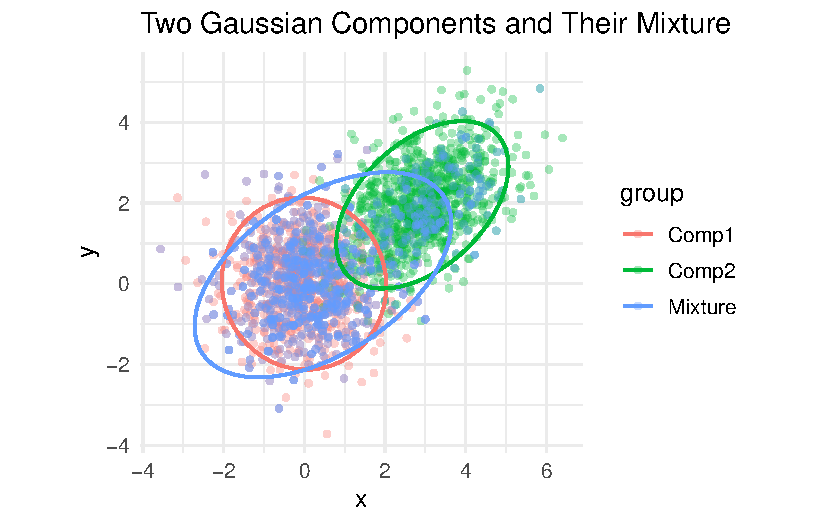
\includegraphics[keepaspectratio]{03-generating-rv_files/figure-pdf/MVN-efficient-1.pdf}}

\end{tcolorbox}

\begin{tcolorbox}[enhanced jigsaw, colbacktitle=quarto-callout-note-color!10!white, coltitle=black, opacityback=0, toprule=.15mm, titlerule=0mm, breakable, bottomtitle=1mm, bottomrule=.15mm, colframe=quarto-callout-note-color-frame, leftrule=.75mm, rightrule=.15mm, arc=.35mm, title=\textcolor{quarto-callout-note-color}{\faInfo}\hspace{0.5em}{Higher dimensional case}, left=2mm, opacitybacktitle=0.6, toptitle=1mm, colback=white]

It is difficult to visualize data in \(R^d\), for \(d\ge 4\), so we
display only the histograms of the marginal distributions. All of the
one-dimensional marginal distributions are univariate normal location
mixtures.

\begin{Shaded}
\begin{Highlighting}[]
\FunctionTok{set.seed}\NormalTok{(}\DecValTok{777}\NormalTok{)}
\FunctionTok{library}\NormalTok{(MASS)}
\FunctionTok{library}\NormalTok{(ggplot2)}
\FunctionTok{library}\NormalTok{(tidyr)}

\CommentTok{\# {-}{-}{-}{-} generate x exactly like your call {-}{-}{-}{-}}
\NormalTok{x }\OtherTok{\textless{}{-}} \FunctionTok{loc.mix}\NormalTok{(}\DecValTok{1000}\NormalTok{, .}\DecValTok{5}\NormalTok{, }\FunctionTok{rep}\NormalTok{(}\DecValTok{0}\NormalTok{, }\DecValTok{4}\NormalTok{), }\DecValTok{2}\SpecialCharTok{:}\DecValTok{5}\NormalTok{, }\AttributeTok{Sigma =} \FunctionTok{diag}\NormalTok{(}\DecValTok{4}\NormalTok{))}
\FunctionTok{colnames}\NormalTok{(x) }\OtherTok{\textless{}{-}} \FunctionTok{paste0}\NormalTok{(}\StringTok{"X"}\NormalTok{, }\DecValTok{1}\SpecialCharTok{:}\DecValTok{4}\NormalTok{)}

\CommentTok{\# {-}{-}{-}{-} ggplot histograms {-}{-}{-}{-}}
\NormalTok{r }\OtherTok{\textless{}{-}} \FunctionTok{range}\NormalTok{(x) }\SpecialCharTok{*} \FloatTok{1.2}  \CommentTok{\# global x{-}limits like your base R code}
\NormalTok{df\_long }\OtherTok{\textless{}{-}} \FunctionTok{as.data.frame}\NormalTok{(x) }\SpecialCharTok{|\textgreater{}}
  \FunctionTok{pivot\_longer}\NormalTok{(}\FunctionTok{everything}\NormalTok{(), }\AttributeTok{names\_to =} \StringTok{"Variable"}\NormalTok{, }\AttributeTok{values\_to =} \StringTok{"Value"}\NormalTok{)}

\FunctionTok{ggplot}\NormalTok{(df\_long, }\FunctionTok{aes}\NormalTok{(}\AttributeTok{x =}\NormalTok{ Value)) }\SpecialCharTok{+}
  \FunctionTok{geom\_histogram}\NormalTok{(}\FunctionTok{aes}\NormalTok{(}\AttributeTok{y =}\NormalTok{ ..density..),}
                 \AttributeTok{breaks =} \FunctionTok{seq}\NormalTok{(}\SpecialCharTok{{-}}\DecValTok{5}\NormalTok{, }\DecValTok{10}\NormalTok{, }\FloatTok{0.5}\NormalTok{),}
                 \AttributeTok{fill =} \StringTok{"red"}\NormalTok{, }\AttributeTok{color =} \StringTok{"white"}\NormalTok{) }\SpecialCharTok{+}
  \FunctionTok{facet\_wrap}\NormalTok{(}\SpecialCharTok{\textasciitilde{}}\NormalTok{ Variable, }\AttributeTok{ncol =} \DecValTok{2}\NormalTok{) }\SpecialCharTok{+}
  \FunctionTok{coord\_cartesian}\NormalTok{(}\AttributeTok{xlim =}\NormalTok{ r, }\AttributeTok{ylim =} \FunctionTok{c}\NormalTok{(}\DecValTok{0}\NormalTok{, }\FloatTok{0.3}\NormalTok{)) }\SpecialCharTok{+}
  \FunctionTok{theme\_minimal}\NormalTok{(}\AttributeTok{base\_size =} \DecValTok{12}\NormalTok{) }\SpecialCharTok{+}
  \FunctionTok{labs}\NormalTok{(}
    \AttributeTok{title =} \StringTok{"Histograms of a 4D Gaussian Location Mixture"}\NormalTok{,}
    \AttributeTok{subtitle =} \FunctionTok{expression}\NormalTok{(}\FunctionTok{paste}\NormalTok{(}\StringTok{"p = 0.5,  "}\NormalTok{, mu[}\DecValTok{1}\NormalTok{], }\StringTok{" = (0,0,0,0),  "}\NormalTok{,}
\NormalTok{                                mu[}\DecValTok{2}\NormalTok{], }\StringTok{" = (2,3,4,5),  "}\NormalTok{,}
\NormalTok{                                Sigma, }\StringTok{" = I"}\NormalTok{)),}
    \AttributeTok{x =} \StringTok{"Value"}\NormalTok{, }\AttributeTok{y =} \StringTok{"Density"}
\NormalTok{  )}
\end{Highlighting}
\end{Shaded}

\begin{verbatim}
Warning: The dot-dot notation (`..density..`) was deprecated in ggplot2 3.4.0.
i Please use `after_stat(density)` instead.
\end{verbatim}

\pandocbounded{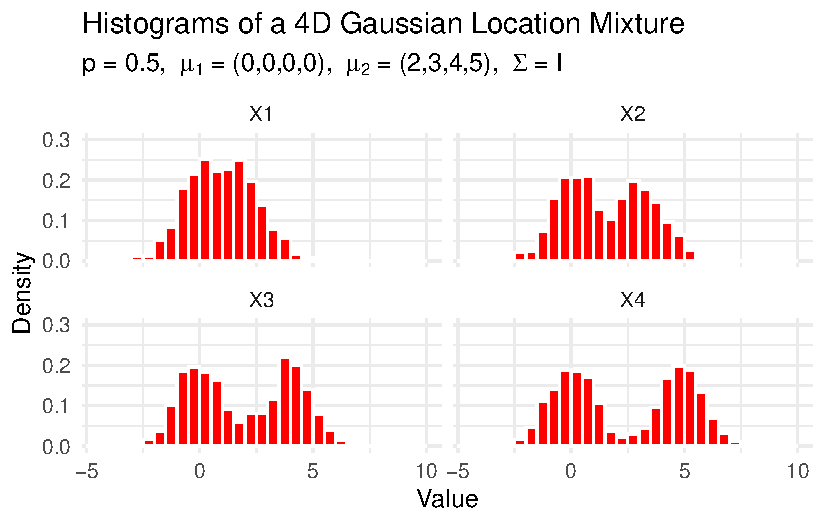
\includegraphics[keepaspectratio]{03-generating-rv_files/figure-pdf/MVN-HD-1.pdf}}

\end{tcolorbox}

\subsection{Uniform Distribution on a
Sphere}\label{uniform-distribution-on-a-sphere}

The uniform distribution on the surface of a \(d\)-sphere in
\(\mathbb{R}^d\) is the distribution that assigns equal probability to
equal areas on the surface of the sphere.

The d-sphere is the set of all points \(x \in R^d\) such that
\(\| x \| = \sqrt{x^\top x) = 1\). Random vectors uniformly distributed
on the \(d\)-sphere have equally likely directions. A method of
generating this distribution uses a property of the

multivariate normal distribution (see {[}97, 160{]}). If X1, . . . , Xd
are iid N (0, 1), then U = (U1, . . . , Ud) is uniformly distributed on
the unit sphere in Rd, where

\[
U_j=\frac{X_j}{\left(X_1^2+\cdots+X_d^2\right)^{1 / 2}}, \quad j=1, \ldots, d \tag{*}
\]

Algorithm to generate uniform variates on the \(d\)-Sphere

\begin{enumerate}
\def\labelenumi{\arabic{enumi}.}
\tightlist
\item
  For each variate \(u_i,~ i = 1,\dots , n\) repeat
\end{enumerate}

\begin{enumerate}
\def\labelenumi{(\alph{enumi})}
\item
  Generate a random sample \(x_{i_1}, \dots , x_{i_d}\) from
  \(N (0, 1)\).
\item
  Compute the Euclidean norm
  \(\|x_i\| = (x^2_{i1} + \cdots + x^2_{id})^{1/2}\).
\item
  Set \(u_{ij} = x_{ij} / \|xi\|, j = 1, \dots , d\).
\item
  Deliver \(u_i = (u_{i1}, \dots , u_{id})\).
\end{enumerate}

To implement these steps efficiently in \textbf{R} for a sample size n,

\begin{enumerate}
\def\labelenumi{\arabic{enumi}.}
\item
  Generate nd univariate normals in \(n \times d\) matrix \(M\). The
  \(i\)th row of M corresponds to the ith random vector \(u_i\).
\item
  Compute the denominator of (*) for each row, storing the \(n\) norms
  in vector \(L\).
\item
  Divide each number M{[}i,j{]} by the norm L{[}i{]}, to get the matrix
  U, where \(U[i,] = u_i = (u_{i1}, \dots, u_{id})\).
\item
  Deliver matrix \(U\) containing \(n\) random observations in rows.
\end{enumerate}

This example provides a function to generate random variates uniformly
distributed on the unit \(d\)-sphere.

\begin{Shaded}
\begin{Highlighting}[]
\NormalTok{runif.sphere }\OtherTok{\textless{}{-}} \ControlFlowTok{function}\NormalTok{(n, d) \{}
  \CommentTok{\# return a random sample uniformly distributed}
  \CommentTok{\# on the unit sphere in R \^{}d}
\NormalTok{  M }\OtherTok{\textless{}{-}} \FunctionTok{matrix}\NormalTok{(}\FunctionTok{rnorm}\NormalTok{(n }\SpecialCharTok{*}\NormalTok{ d), }\AttributeTok{nrow =}\NormalTok{ n, }\AttributeTok{ncol =}\NormalTok{ d)}
\NormalTok{  L }\OtherTok{\textless{}{-}} \FunctionTok{apply}\NormalTok{(M,}
    \AttributeTok{MARGIN =} \DecValTok{1}\NormalTok{,}
    \AttributeTok{FUN =} \ControlFlowTok{function}\NormalTok{(x) \{}
      \FunctionTok{sqrt}\NormalTok{(}\FunctionTok{sum}\NormalTok{(x }\SpecialCharTok{*}\NormalTok{ x))}
\NormalTok{    \}}
\NormalTok{  )}
\NormalTok{  D }\OtherTok{\textless{}{-}} \FunctionTok{diag}\NormalTok{(}\DecValTok{1} \SpecialCharTok{/}\NormalTok{ L)}
\NormalTok{  U }\OtherTok{\textless{}{-}}\NormalTok{ D }\SpecialCharTok{\%*\%}\NormalTok{ M}
\NormalTok{  U}
\NormalTok{\}}

\CommentTok{\#generate a sample in d=2 and plot}
\NormalTok{X\_d2 }\OtherTok{\textless{}{-}} \FunctionTok{runif.sphere}\NormalTok{(}\DecValTok{200}\NormalTok{, }\DecValTok{2}\NormalTok{)}
\NormalTok{df }\OtherTok{\textless{}{-}} \FunctionTok{data.frame}\NormalTok{(}\AttributeTok{x1 =}\NormalTok{ X\_d2[,}\DecValTok{1}\NormalTok{], }\AttributeTok{x2 =}\NormalTok{ X\_d2[,}\DecValTok{2}\NormalTok{])}

\FunctionTok{ggplot}\NormalTok{(df, }\FunctionTok{aes}\NormalTok{(}\AttributeTok{x =}\NormalTok{ x1, }\AttributeTok{y =}\NormalTok{ x2)) }\SpecialCharTok{+}
  \FunctionTok{geom\_point}\NormalTok{(}\AttributeTok{color =} \StringTok{"steelblue"}\NormalTok{, }\AttributeTok{size =} \DecValTok{2}\NormalTok{, }\AttributeTok{alpha =} \FloatTok{0.7}\NormalTok{) }\SpecialCharTok{+}
  \FunctionTok{coord\_equal}\NormalTok{() }\SpecialCharTok{+}                     
  \FunctionTok{labs}\NormalTok{(}
    \AttributeTok{x =} \FunctionTok{expression}\NormalTok{(x[}\DecValTok{1}\NormalTok{]),}
    \AttributeTok{y =} \FunctionTok{expression}\NormalTok{(x[}\DecValTok{2}\NormalTok{]),}
    \AttributeTok{title =} \StringTok{"Uniform Random Points on the Unit Circle"}
\NormalTok{  ) }\SpecialCharTok{+}
\NormalTok{  ggforce}\SpecialCharTok{::}\FunctionTok{geom\_circle}\NormalTok{(}\FunctionTok{aes}\NormalTok{(}\AttributeTok{x0 =} \DecValTok{0}\NormalTok{, }\AttributeTok{y0 =} \DecValTok{0}\NormalTok{, }\AttributeTok{r =} \DecValTok{1}\NormalTok{), }\AttributeTok{inherit.aes =} \ConstantTok{FALSE}\NormalTok{,}
              \AttributeTok{color =} \StringTok{"black"}\NormalTok{, }\AttributeTok{linetype =} \StringTok{"dashed"}\NormalTok{)}
\end{Highlighting}
\end{Shaded}

\begin{verbatim}
Warning in ggforce::geom_circle(aes(x0 = 0, y0 = 0, r = 1), inherit.aes = FALSE, : All aesthetics have length 1, but the data has 200 rows.
i Please consider using `annotate()` or provide this layer with data containing
  a single row.
\end{verbatim}

\pandocbounded{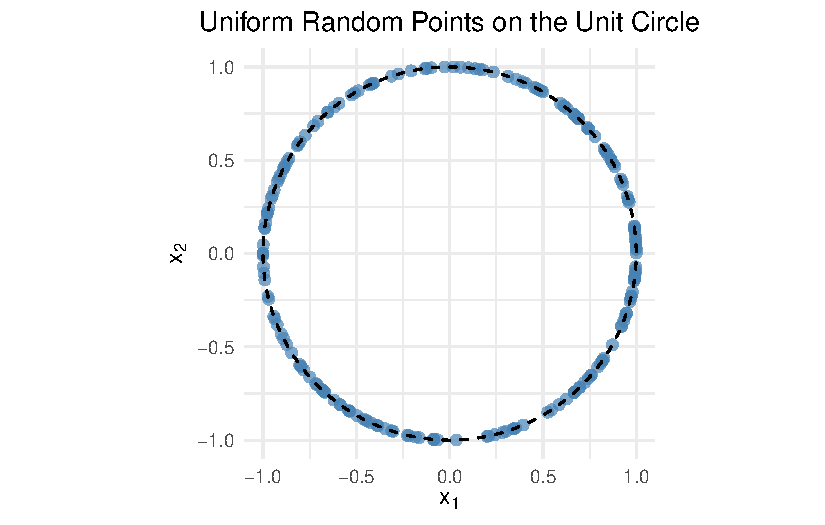
\includegraphics[keepaspectratio]{03-generating-rv_files/figure-pdf/sphere-1.pdf}}

\begin{center}\rule{0.5\linewidth}{0.5pt}\end{center}

Reference used:

\begin{itemize}
\tightlist
\item
  Rizzo, M.L. (2007)
  \href{https://a-roshani.ir/files/SC/\%5B4\%5D\%20\%5BMaria\%20L.\%20Rizzo\%5D\%5B2019\%5D\%20Statistical\%20Computing\%20\%20with\%20R,\%20Second\%20Edition.pdf}{\emph{Statistical
  Computing with R}}. CRC Press, Roca Baton.
\end{itemize}

\bookmarksetup{startatroot}

\chapter{Monte Carlo Simulation and Variance
Reduction}\label{monte-carlo-simulation-and-variance-reduction}

\newcommand{\unif}{\operatorname{Unif}}
\newcommand{\E}{\mathbb{E}}
\newcommand{\var}{\mathbb{V}ar}
\newcommand{\geom}{\operatorname{Geom}}
\newcommand{\beta}{\operatorname{Beta}}
\newcommand{\bern}{\operatorname{Bern}}
\newcommand{\R}{\mathbb{R}}
\newcommand{\iid}{\overset{iid}{\sim}}
\newcommand{\cov}{\mathbb{C}ov}
\newcommand{\eff}{\operatorname{Eff}}
\newcommand{\htt}{\hat{\theta}}

Monte Carlo (MC) integration is a simulation-based method for
\emph{approximating integrals} using random sampling.

In numerical integration, methods such as the trapezoidal rule use a
\emph{deterministic approach}. MC integration, on the other hand,
employs a \emph{non-deterministic} approach: each realization provides a
different outcome.

\section{What is Monte Carlo
Simulation?}\label{what-is-monte-carlo-simulation}

\subsection{History}\label{history}

Monte Carlo (MC) is a casino in Monaco, famous for its gambling and
games of chance. The term ``Monte Carlo'' was coined by physicists
Stanislaw Ulam in the 1940s while working on nuclear weapon projects at
Los Almos.

\begin{figure}[H]

{\centering \pandocbounded{\includegraphics[keepaspectratio]{index_files/mediabag/640px-Table_de_Roule.jpg}}

}

\caption{Monte Carlo Casino, Picture borrowed from Wikipedia}

\end{figure}%

Monte Carlo methods are mainly used in three distinct problem classes:

\begin{enumerate}
\def\labelenumi{\arabic{enumi}.}
\item
  optimization
\item
  numerical integration
\item
  generating draws from a probability distribution.
\end{enumerate}

They can also be used to model phenomena with significant uncertainty in
inputs, such as calculating the risk of a nuclear power plant failure.
Monte Carlo methods are often implemented using computer simulations,
and they can provide approximate solutions to problems that are
otherwise intractable or too complex to analyze mathematically.

\subsection{Key Steps of MC methods}\label{key-steps-of-mc-methods}

Monte Carlo methods vary, but tend to follow a particular pattern:

\begin{enumerate}
\def\labelenumi{\arabic{enumi}.}
\item
  Define a domain of possible inputs.
\item
  Generate inputs randomly from a probability distribution over the
  domain.
\item
  Perform a deterministic computation of the outputs.
\item
  Aggregate the results.
\end{enumerate}

For example, consider a quadrant (circular sector) inscribed in a unit
square. Given that the ratio of their areas is
\$\pi/4\(4⁠, the value o f\)\piπ can be approximated using the Monte
Carlo method:

\begin{enumerate}
\def\labelenumi{\arabic{enumi}.}
\item
  Draw a square, then inscribe a quadrant within it.
\item
  Uniformly scatter a given number of points over the square.
\item
  Count the number of points inside the quadrant, i.e.~having a distance
  from the origin of less than 1.
\item
  The ratio of the inside-count and the total-sample-count is an
  estimate of the ratio of the two areas, ⁠π/4⁠. Multiply the result by 4
  to estimate π.
\end{enumerate}

\begin{figure}[H]

{\centering \pandocbounded{\includegraphics[keepaspectratio]{index_files/mediabag/660px-Pi_monte_carlo.gif}}

}

\caption{Picture borrowed from Wikipedia}

\end{figure}%

\section{Basic Monte Carlo
Integration}\label{basic-monte-carlo-integration}

To approximate the integral of a function \(f(x)\) over the interval
\([a, b]\), we can use the following formula:

Consider the problem of estimating \(\theta = \int_0^1 g(x)dx\). If
\(X_1,\dots , X_m\sim\operatorname{Unif}(0,1)\), then the MC estimator
is given by:

\[\hat{\theta}=\bar{g}_m(X)=\frac{1}{m}\sum_{i=1}^m g(X_i)\] converges
to \(\mathbb{E}[g(X)]\) as \(m\to\infty\) with probability 1, by
\emph{Strong law of Large Number} (SLLN). The simple MC estimator is
unbiased, i.e., \(\bar{g}_m(X)\).

Compute a MC estimate \[
\theta = \int_0^1 \exp(-x)dx,
\] and compare the estimate with the theoretical value

\begin{Shaded}
\begin{Highlighting}[]
\FunctionTok{set.seed}\NormalTok{(}\DecValTok{777}\NormalTok{)}
\NormalTok{n }\OtherTok{\textless{}{-}} \FloatTok{1E3}
\NormalTok{x }\OtherTok{\textless{}{-}} \FunctionTok{runif}\NormalTok{(n)}
\CommentTok{\# simulated estimator}
\NormalTok{theta\_hat }\OtherTok{\textless{}{-}} \FunctionTok{exp}\NormalTok{(}\SpecialCharTok{{-}}\NormalTok{x) }\SpecialCharTok{|\textgreater{}} \FunctionTok{mean}\NormalTok{()}

\CommentTok{\# theoretical value}
\NormalTok{theta\_true }\OtherTok{\textless{}{-}} \DecValTok{1} \SpecialCharTok{{-}} \FunctionTok{exp}\NormalTok{(}\SpecialCharTok{{-}}\DecValTok{1}\NormalTok{)}

\CommentTok{\# put them in a tibble}
\NormalTok{(results }\OtherTok{\textless{}{-}} \FunctionTok{tibble}\NormalTok{(}
  \AttributeTok{Method =} \FunctionTok{c}\NormalTok{(}\StringTok{"Simulated"}\NormalTok{, }\StringTok{"Theoretical"}\NormalTok{),}
  \AttributeTok{Value  =} \FunctionTok{c}\NormalTok{(theta\_hat, theta\_true)))}
\end{Highlighting}
\end{Shaded}

\begin{verbatim}
# A tibble: 2 x 2
  Method      Value
  <chr>       <dbl>
1 Simulated   0.641
2 Theoretical 0.632
\end{verbatim}

To simulate \(\int_a^b g(t)dt\), use change of variable so the limit
becomes from \(0\) to \(1\). This can be done through a \emph{linear
transformation} of the variable \(t\): \(y:=\frac{t-a}{b-a}\). Then,
\(t=a+(b-a)y\) and \(dt=(b-a)dy\). Thus, we have \[
\int_a^b g(t)dt = (b-a)\int_0^1 g(a+(b-a)y)dy.
\] Alternatively, instead of using \(\operatorname{Unif}(0,1)\), we can
replace it with other densities with supports between \(a\) and \(b\).
One instance is, \[
\int_a^b g(t)dt = \int_a^b \frac{g(t)}{f}f dt = (b-a) \int_a^b  \frac{g(t)}{b-a} dt.
\] This is a \(b-a\) times the expectation of \(g(X)\) where
\(X\sim \operatorname{Unif}(a,b)\). Therefore, this integral can be
estimated by averaging through the function \(g(\cdot)\) over the
interval from \(a\) to \(b\) multiply by \(b-a\).

Compute a MC estimate of \[
\theta = \int_2^4 \exp(-x)dx,
\] and compare the estimate with the exact value of the integral.

\begin{Shaded}
\begin{Highlighting}[]
\FunctionTok{library}\NormalTok{(tibble)}

\FunctionTok{set.seed}\NormalTok{(}\DecValTok{777}\NormalTok{)}
\NormalTok{m }\OtherTok{\textless{}{-}} \FloatTok{1E3}
\NormalTok{x }\OtherTok{\textless{}{-}} \FunctionTok{runif}\NormalTok{(m, }\AttributeTok{min =} \DecValTok{2}\NormalTok{, }\AttributeTok{max =} \DecValTok{4}\NormalTok{)}

\CommentTok{\# simulated estimator}
\NormalTok{theta\_hat }\OtherTok{\textless{}{-}} \FunctionTok{exp}\NormalTok{(}\SpecialCharTok{{-}}\NormalTok{x) }\SpecialCharTok{|\textgreater{}} \FunctionTok{mean}\NormalTok{() }\SpecialCharTok{*}\NormalTok{ (}\DecValTok{4} \SpecialCharTok{{-}} \DecValTok{2}\NormalTok{)}

\CommentTok{\# theoretical value}
\NormalTok{theta\_true }\OtherTok{\textless{}{-}} \FunctionTok{exp}\NormalTok{(}\SpecialCharTok{{-}}\DecValTok{2}\NormalTok{) }\SpecialCharTok{{-}} \FunctionTok{exp}\NormalTok{(}\SpecialCharTok{{-}}\DecValTok{4}\NormalTok{)}

\CommentTok{\# put into tibble}
\NormalTok{(results }\OtherTok{\textless{}{-}} \FunctionTok{tibble}\NormalTok{(}
  \AttributeTok{Method =} \FunctionTok{c}\NormalTok{(}\StringTok{"Simulated"}\NormalTok{, }\StringTok{"Theoretical"}\NormalTok{),}
  \AttributeTok{Value  =} \FunctionTok{c}\NormalTok{(theta\_hat, theta\_true)}
\NormalTok{))}
\end{Highlighting}
\end{Shaded}

\begin{verbatim}
# A tibble: 2 x 2
  Method      Value
  <chr>       <dbl>
1 Simulated   0.120
2 Theoretical 0.117
\end{verbatim}

To summarize, the simple Monte Carlo estimator of the integral
\(\theta = \int_a^b g(x)dx\) is computed as follows.

\begin{enumerate}
\def\labelenumi{\arabic{enumi}.}
\item
  Generate
  \(X_1, \dots , X_m\overset{iid}{\sim}\operatorname{Unif}(a,b)\),
\item
  Compute \(\bar{g}(X) = \frac{1}{m} g(X_i)\).
\item
  \(\hat{\theta} = (b − a)\bar{g}(X)\).
\end{enumerate}

Compute a MC estimate of a standard normal cdf

\[
\Phi(x)=\int_{-\infty}^x \frac{1}{\sqrt{2 \pi}} e^{-t^2 / 2} d t
\]

\begin{enumerate}
\def\labelenumi{\arabic{enumi}.}
\tightlist
\item
  Note, we cannot apply the algorithm above directly because the limits
  of integration cover an \emph{unbounded interval}. However, we can
  break this problem into two cases: (i) \(x \ge 0\) and (ii) \(x < 0\),
  and use the \emph{symmetry} of the normal density to handle the second
  case. Then the problem is to estimate
  \(\theta =\int_0^x \theta = \int_0^x \exp(−t^2/2) dt\) for \(x > 0\).
  This can be done by generating random \(\operatorname{Unif}(0,x)\)
  numbers, but it would mean changing the parameters of the uniform
  distribution for each different value of the cdf required. Suppose
  that we prefer an algorithm that always samples from
  \(\operatorname{Unif}(0,1)\). This can be accomplished by a change of
  variables. Making the substitution \(y = t/x\), we have \(dt = x dy\)
  and
\end{enumerate}

\[
\theta=\int_0^1 x e^{-(x y)^2 / 2} d y
\] Thus, \(\theta = \mathbb{E}_Y[x\exp(-(xY)^2/2)]\), where the rv
\(Y\sim \operatorname{Unif}(0,1)\). Generate iid
\(\operatorname{Unif}(0,1)\) random numbers \(u_1,\dots,u_m\), and
compute
\[\hat{\theta}=\overline{g_m(u)}=\frac{1}{m} \sum_{i=1}^m x e^{-\left(u_i x\right)^2 / 2}.
\]

The sample mean \(\hat{\theta}\) converges to
\(\mathbb{E}\hat{\theta} = \theta\) as \(m\to \infty\). If \(x > 0\),
the estimate of \(\Phi(x) = 1/2 + \hat{\theta}/\sqrt{2\pi}\). If
\(x < 0\) compute \(\Phi(x) = 1 − \Phi(−x)\).

\begin{Shaded}
\begin{Highlighting}[]
\NormalTok{x }\OtherTok{\textless{}{-}} \FunctionTok{seq}\NormalTok{(.}\DecValTok{1}\NormalTok{, }\FloatTok{2.5}\NormalTok{, }\AttributeTok{length =} \DecValTok{10}\NormalTok{)}
\NormalTok{m }\OtherTok{\textless{}{-}} \DecValTok{10000}
\NormalTok{u }\OtherTok{\textless{}{-}} \FunctionTok{runif}\NormalTok{(m)}
\NormalTok{cdf }\OtherTok{\textless{}{-}} \FunctionTok{numeric}\NormalTok{(}\FunctionTok{length}\NormalTok{(x))}
\ControlFlowTok{for}\NormalTok{ (i }\ControlFlowTok{in} \DecValTok{1}\SpecialCharTok{:}\FunctionTok{length}\NormalTok{(x)) \{}
\NormalTok{  g }\OtherTok{\textless{}{-}}\NormalTok{ x[i] }\SpecialCharTok{*} \FunctionTok{exp}\NormalTok{(}\SpecialCharTok{{-}}\NormalTok{(u }\SpecialCharTok{*}\NormalTok{ x[i])}\SpecialCharTok{\^{}}\DecValTok{2} \SpecialCharTok{/} \DecValTok{2}\NormalTok{)}
\NormalTok{  cdf[i] }\OtherTok{\textless{}{-}} \FunctionTok{mean}\NormalTok{(g) }\SpecialCharTok{/} \FunctionTok{sqrt}\NormalTok{(}\DecValTok{2} \SpecialCharTok{*}\NormalTok{ pi) }\SpecialCharTok{+} \FloatTok{0.5}
\NormalTok{\}}
\NormalTok{Phi }\OtherTok{\textless{}{-}} \FunctionTok{pnorm}\NormalTok{(x)}
\FunctionTok{print}\NormalTok{(}\FunctionTok{round}\NormalTok{(}\FunctionTok{rbind}\NormalTok{(x, cdf, Phi), }\DecValTok{3}\NormalTok{))}
\end{Highlighting}
\end{Shaded}

\begin{verbatim}
    [,1]  [,2]  [,3]  [,4]  [,5]  [,6]  [,7]  [,8]  [,9] [,10]
x   0.10 0.367 0.633 0.900 1.167 1.433 1.700 1.967 2.233 2.500
cdf 0.54 0.643 0.737 0.816 0.878 0.924 0.956 0.976 0.987 0.994
Phi 0.54 0.643 0.737 0.816 0.878 0.924 0.955 0.975 0.987 0.994
\end{verbatim}

Notice that it would have been simpler to generate random Uniform(0, x)
random variables and skip the transformation. In fact, the integrand of
the previous example is itself a density function, and we can generate
random variables from this density. This provides a more direct approach
to estimating the integral.

Let \(I(\cdot)\) be the indicator function, and \(Z\sim N(0,1)\). Then
for any constant \(x\) we have
\(\mathbb{E}[I(Z ≤ x)] = P (Z ≤ x) =\Phi(x)\), the standard normal cdf
evaluated at \(x\).

Generate a random sample \(z_1, \dots , z_m\sim N(0,1)\). Then the
theoretical mean and sample mean are
\[\hat{\theta} = \frac{1}{m} \sum_{i=1}^m I(z_i \le x),\] and
\[\mathbb{E}[\hat{\theta}] = P(Z \le x) = \Phi(x).\]

\begin{Shaded}
\begin{Highlighting}[]
\FunctionTok{set.seed}\NormalTok{(}\DecValTok{777}\NormalTok{)}
\NormalTok{x }\OtherTok{\textless{}{-}} \FunctionTok{seq}\NormalTok{(}\FloatTok{0.1}\NormalTok{, }\FloatTok{2.5}\NormalTok{, }\AttributeTok{length =} \DecValTok{10}\NormalTok{)}
\NormalTok{m }\OtherTok{\textless{}{-}} \FloatTok{1E4}
\NormalTok{z }\OtherTok{\textless{}{-}} \FunctionTok{rnorm}\NormalTok{(m)}
\FunctionTok{dim}\NormalTok{(x) }\OtherTok{\textless{}{-}} \FunctionTok{length}\NormalTok{(x)}
\NormalTok{p }\OtherTok{\textless{}{-}} \FunctionTok{apply}\NormalTok{(x, }\AttributeTok{MARGIN =} \DecValTok{1}\NormalTok{,}
  \AttributeTok{FUN =} \ControlFlowTok{function}\NormalTok{(x, z) \{}\FunctionTok{mean}\NormalTok{(z }\SpecialCharTok{\textless{}}\NormalTok{ x)\}, }\AttributeTok{z =}\NormalTok{ z)}
\NormalTok{Phi }\OtherTok{\textless{}{-}} \FunctionTok{pnorm}\NormalTok{(x)}

\FunctionTok{rbind}\NormalTok{(x, p, Phi) }\SpecialCharTok{|\textgreater{}} \FunctionTok{round}\NormalTok{(}\DecValTok{3}\NormalTok{)}
\end{Highlighting}
\end{Shaded}

\begin{verbatim}
     [,1]  [,2]  [,3]  [,4]  [,5]  [,6]  [,7]  [,8]  [,9] [,10]
x   0.100 0.367 0.633 0.900 1.167 1.433 1.700 1.967 2.233 2.500
p   0.544 0.645 0.740 0.818 0.881 0.926 0.957 0.976 0.986 0.993
Phi 0.540 0.643 0.737 0.816 0.878 0.924 0.955 0.975 0.987 0.994
\end{verbatim}

In this example, compared with the previous example, it appears that we
have better agreement with \texttt{pnorm()} in the upper tail, but worse
agreement near the center.

\begin{tcolorbox}[enhanced jigsaw, colbacktitle=quarto-callout-note-color!10!white, coltitle=black, opacityback=0, toprule=.15mm, titlerule=0mm, breakable, bottomtitle=1mm, bottomrule=.15mm, colframe=quarto-callout-note-color-frame, leftrule=.75mm, rightrule=.15mm, arc=.35mm, title=\textcolor{quarto-callout-note-color}{\faInfo}\hspace{0.5em}{Note}, left=2mm, opacitybacktitle=0.6, toptitle=1mm, colback=white]

Summarizing, if \(f (x)\) is a probability density function supported on
a set A, (that is, \(f (x) \ge 0\) for all \(x\in\mathbb{R}\) and
\(\int_A f (x) = 1\)), to estimate the integral
\[\theta = \int_A g(x)f (x)dx,\] generate a random sample
\(x_1,\dots,x_m\) from the distribution \(f (x)\), and compute the
sample mean \[\hat{\theta} = \frac{1}{m}\sum_{i=1}^mg(x_i).\] Then
\(\hat{\theta}\overset{p}{\to}\theta\) by the weak law of large numbers
(WLLN).

\end{tcolorbox}

The standard error of \(\hat{\theta} = \frac{1}{m}\sum_{i=1}^m g(x_i)\).

Recall that, \(\mathbb{V}ar({\hat{\theta}})=\sigma^2/m\) where
\(\sigma^2 = \mathbb{V}ar\{g(X)\}\). When the distribution of \(X\) is
unknown, we substitute for \(F_X\) the empirical distribution \(F_m\) of
the sample \(x_1, \dots , x_m\). The variance of \(\hat{\theta}\) can be
estimated by \[
\frac{\hat{\sigma}^2}{m} = \frac{1}{m^2}\sum_{i=1}^m [g(x_i) - \bar{g}(x)]^2.
\]

Note that \[\frac{1}{m}\sum_{i=1}^m[g(x_i)-\bar{g}(x_i)]^2,\] is the
\emph{plug-in estimate} of \(\mathbb{V}ar\{g(X)\}\). That is, it is the
variance of \(U\) , where \(U\) is uniformly distributed on the set of
replicates \(\{g(x_i)\}\). The corresponding estimated standard error of
\(\hat{\theta}\) is \[
\widehat{se}(\hat{\theta}) = \frac{\hat{\sigma}}{\sqrt{m}} = \frac{1}{m}\left\{\sum_{i=1}^m [ g(x_i)- \bar{g}(x)]^2\right\}^{1/2}.
\] The CLT implies \[
\frac{\hat{\theta}-E[\hat{\theta}]}{\sqrt{\mathbb{V}ar(\hat{\theta})}} \overset{D}{\to} N(0,1),
\] as \(m\to\infty\). Hence, if \(m\) is sufficiently large,
\(\hat{\theta}\) is approximately normal with mean \(\theta\). The
large-sample, approximately normal distribution of \(\hat{\theta}\) can
be applied to put confidence limits or error bounds on the MC estimate
of the integral, and check for convergence

Compute the 95\% confidence interval for \(\Phi(2)\) and \(\Phi(2.5)\).

\begin{Shaded}
\begin{Highlighting}[]
\FunctionTok{set.seed}\NormalTok{(}\DecValTok{777}\NormalTok{)}
\NormalTok{x }\OtherTok{\textless{}{-}} \DecValTok{2}
\NormalTok{m }\OtherTok{\textless{}{-}} \DecValTok{10000}
\NormalTok{z }\OtherTok{\textless{}{-}} \FunctionTok{rnorm}\NormalTok{(m)}
\NormalTok{g }\OtherTok{\textless{}{-}}\NormalTok{ (z }\SpecialCharTok{\textless{}}\NormalTok{ x) }\CommentTok{\#the indicator function}
\NormalTok{v }\OtherTok{\textless{}{-}} \FunctionTok{mean}\NormalTok{((g }\SpecialCharTok{{-}} \FunctionTok{mean}\NormalTok{(g))}\SpecialCharTok{\^{}}\DecValTok{2}\NormalTok{) }\SpecialCharTok{/}\NormalTok{ m}
\NormalTok{cdf }\OtherTok{\textless{}{-}} \FunctionTok{mean}\NormalTok{(g)}
\FunctionTok{c}\NormalTok{(cdf, v)}
\end{Highlighting}
\end{Shaded}

\begin{verbatim}
[1] 9.771000e-01 2.237559e-06
\end{verbatim}

\begin{Shaded}
\begin{Highlighting}[]
\FunctionTok{c}\NormalTok{(cdf }\SpecialCharTok{{-}} \FloatTok{1.96} \SpecialCharTok{*} \FunctionTok{sqrt}\NormalTok{(v), cdf }\SpecialCharTok{+} \FloatTok{1.96} \SpecialCharTok{*} \FunctionTok{sqrt}\NormalTok{(v))}
\end{Highlighting}
\end{Shaded}

\begin{verbatim}
[1] 0.9741681 0.9800319
\end{verbatim}

The interpretation is:

the probability \(P (I(Z < x) = 1)\) is \(\Phi(2)\approx 0.977\). Here
\(g(X)\) has the distribution of the sample proportion of 1's in
\(m = 10000\) Bernoulli trials with \(p\approx 0.977\), and the variance
of \(g(X)\) is therefore
\((0.977)(1 − 0.977)/10000 =2.223 \times 10^{-6}\). The MC estimate
\(2.228\times 10^{-6}\) of variance is quite close to this value.

Q: What about \(\Phi(2.5)\)?

\section{Variance and Efficiency}\label{variance-and-efficiency}

We have seen that a MC approach to estimating the integral
\(\int_a^b g(x)dx\) is to represent the integral as the expected value
of a function of a uniform random variable. That is, suppose
\(X\sim \operatorname{Unif}(0,1)\), then \(f(x) = (b-a)^{-1}\) for
\(x\in[a,b]\) and 0 otherwise, and \[
\begin{aligned}
\theta & =\int_a^b g(x) d x \\
& =(b-a) \int_a^b g(x) \frac{1}{b-a} d x=(b-a) E[g(X)]
\end{aligned}
\]

Recall that, from \emph{Algorithm 2}, the sample-mean MC estimator of
the integral \(\theta\) is computed as follows.

\begin{enumerate}
\def\labelenumi{\arabic{enumi}.}
\item
  Generate
  \(X_1, \dots , X_m\overset{iid}{\sim}\operatorname{Unif}(a,b)\),
\item
  Compute \(\bar{g}(X) = g(X_i)/m\)
\item
  \(\hat{\theta} = (b − a)\bar{g}(X)\).
\end{enumerate}

The sample mean \(\bar{g}(X)\) has expected value \(g(X)=\theta/(b-a)\)
and variance \(\mathbb{V}ar\{\bar{g}(X)\}=\mathbb{V}ar\{g(X)\}/m\). By
CLT, \(\bar{g}(X)\) is approximately normal for large \(m\). Therefore,
the variance of the MC estimator \(\hat{\theta}\) is approximately
normal with mean \(\theta\) and variance \(\mathbb{V}ar\{g(X)\}/m\).

\begin{tcolorbox}[enhanced jigsaw, colbacktitle=quarto-callout-note-color!10!white, coltitle=black, opacityback=0, toprule=.15mm, titlerule=0mm, breakable, bottomtitle=1mm, bottomrule=.15mm, colframe=quarto-callout-note-color-frame, leftrule=.75mm, rightrule=.15mm, arc=.35mm, title=\textcolor{quarto-callout-note-color}{\faInfo}\hspace{0.5em}{Expectation, Variance and Distribution of theta hat}, left=2mm, opacitybacktitle=0.6, toptitle=1mm, colback=white]

The expectation and the variance of the MC estimator \(\hat{\theta}\)
are given by \begin{align*}
\mathbb{E}[\hat{\theta}] & = \theta, \\
\mathbb{V}ar(\hat{\theta}) &= (b-a)^2 \mathbb{V}ar(\overline{g}(X))=\frac{(b-a)^2}{m} \mathbb{V}ar\{g(X)\} .
\end{align*} Further more, by CLT, for large \(m\), \(\overline{g}(X)\)
is approximately normally distributed, and with the mean and variance
given above.

\end{tcolorbox}

\subsection{Hit-or-Miss Approach}\label{hit-or-miss-approach}

The \textbf{``hit-or-miss''} approach to MC integration also uses a
\emph{sample mean} to estimate the integral, but the sample mean is
taken over a \emph{different sample} and \textbf{therefore this
estimator has a different variance than the one we have above}.

\begin{figure}[H]

{\centering \pandocbounded{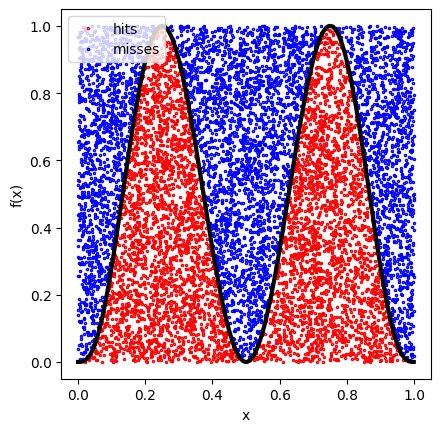
\includegraphics[keepaspectratio]{index_files/mediabag/hZ7K41Jugx8AAAAASUVO.png}}

}

\caption{Hit-or-Miss MC, image borrowed from UBC}

\end{figure}%

Suppose \(f(x)\) is the density of a random variable \(X\). The
``hit-or-miss'' approach to estimating
\(F(x) = \int_{-\infty}^x f(t)\,dt\) is as follows:

\begin{enumerate}
\def\labelenumi{\arabic{enumi}.}
\item
  Generate a random sample \(X_1,\dots,X_m \sim F_X(x)\).
\item
  For each observation \(X_i\), compute \[
  g(X_i) = I(X_i \leq x) =
  \begin{cases}
  1, & X_i \leq x, \\
  0, & X_i > x.
  \end{cases}
  \]
\item
  Compute \[
  \hat{F}(x) = \frac{1}{m} \sum_{i=1}^m I(X_i \leq x).
  \]
\end{enumerate}

Note that the random variable \(Y = g(X) \sim \text{Bern}(1, p)\), where
the success probability is\\
\[
p := P(X \leq x) = F(x).
\]

The transformed sample \(Y_1, \ldots, Y_m\) are the outcomes of \$ m\$
independent, identically distributed Bernoulli trials.

The estimator \(\hat{F}(x)\) is the sample proportion \[
\hat{p} = \frac{y}{m},
\]

where \(y\) is the total number of successes observed in \(m\) trials.
Hence,

\[
\mathbb{E}[\hat{F}(x)] = p = F(x), \qquad 
\mathrm{Var}(\hat{F}(x)) = \frac{p(1-p)}{m} = \frac{F(x)\big(1-F(x)\big)}{m}.
\]

The variance of \(\hat{F}(x)\) can be estimated by \[
\frac{\hat{p}(1-\hat{p})}{m} = \frac{\hat{F}(x)\big(1-\hat{F}(x)\big)}{m}.
\]

The maximum variance occurs when \(F(x) = \tfrac{1}{2}\), so a
conservative estimate of the variance of \(\hat{F}(x)\) is \[
\frac{1}{4m}.
\]

\subsection{Efficiency}\label{efficiency}

Suppose we have two (unbiased) estimators \(\hat{\theta}_1\) and
\(\hat{\theta}_2\) for θ. We say \(\hat{\theta}_1\) is
\emph{statistically} more efficient than \(\hat{\theta}_2\) if
\[\mathbb{V}ar(\hat{\theta}_1) < \mathbb{V}ar(\hat{\theta}_2).\] What is
the variance of \(\hat{\theta}_i\) is unknown or hard to be calculated?

can substitute it by sample estimate of the variance for each estimator.

Note, the variance can \emph{always be reduced by increasing the number
of replicates}, so computational efficiency is also relevant.

\section{Variance Reduction}\label{variance-reduction}

We have seen that MC integration may be used to estimate
\(\theta:=\mathbb{E}[g(X)]\). However, how to have the \emph{efficient
estimator } for \(\theta\), and if we have a several ways
\(\hat{\theta}_1,\dots,\hat{\theta}_k\) to estimate \(\theta\), which
one is \emph{better}, or, more efficient? Here, we try to introduce some
variance reduction techniques.

Let \(\hat{\theta}_1\) and \(\hat{\theta}_2\) be two estimators of
\(\theta\) where
\(\mathbb{V}ar(\hat{\theta}_1) > \mathbb{V}ar(\hat{\theta}_2)\). The
\emph{relative efficiency gain } of \(\hat{\theta_2}\) instead of using
\(\hat{\theta_1}\) is defined as \[
\operatorname{Eff}(\hat{\theta}_1, \hat{\theta}_2) = \frac{\mathbb{V}ar(\hat{\theta}_1)- \mathbb{V}ar(\hat{\theta}_2)}{\mathbb{V}ar(\hat{\theta}_1)}.
\]

Let \(X\) be a random object and let \(g(\cdot)\) be a (possibly
vector--valued) statistic of a \emph{sample} from the distribution of
\(X\). For \(j=1,\ldots,m\), draw an i.i.d. replicate sample
\(X^{(j)}=\{X^{(j)}_1,\ldots,X^{(j)}_n\}\) and compute \[
Y_j = g\!\big(X^{(j)}\big).
\tag{6.5}
\] Then \(Y_1,\ldots,Y_m\) are i.i.d. with common mean \[
\theta \;=\; \mathbb{E}\big[g(X)\big] \;=\; \mathbb{E}[Y].
\]

The MC estimator of \(\theta\) is the sample mean \[
\hat{\theta}\;=\; \bar Y \;=\; \frac{1}{m}\sum_{j=1}^m Y_j.
\] By linearity of expectation, \[
\mathbb{E}[\hat{\theta}] \;=\; \theta,
\] so \(\hat{\theta}\) is unbiased. Its variance is \[
\mathbb{V}ar(\hat{\theta})
  \;=\; \mathbb{V}ar(\bar Y)
  \;=\; \frac{\mathbb{V}ar\{g(X)\}}{m}.
\]

Hence the standard error decays as \(m^{-1/2}\). To reduce the standard
error from \(0.01\) to \(0.0001\), one would need about \(10000\) times
as many replicates. More generally, if \(\mathbb{V}ar\{g(X)\}=\sigma^2\)
and we target standard error at most \(\varepsilon\), then \[
m \;\ge\; \frac{\sigma^2}{\varepsilon^2}
\] replicates suffice (ignoring finite--\(m\) effects).

The remainder of this note gives a minimal simulation illustrating the
\(1/\sqrt{m}\) behavior and provides a template for later
variance--reduction sections (e.g., control variates, antithetic
sampling, importance sampling).

\section{Rule-of-thumb for target standard
error}\label{rule-of-thumb-for-target-standard-error}

Given a target standard error \(\varepsilon\), we can solve
\(\sqrt{\sigma^2/m} \le \varepsilon\) for \(m\).

\begin{Shaded}
\begin{Highlighting}[]
\NormalTok{theta\_true }\OtherTok{\textless{}{-}} \DecValTok{1}
\NormalTok{sigma2\_true }\OtherTok{\textless{}{-}} \DecValTok{2}
\NormalTok{epsilon }\OtherTok{\textless{}{-}} \FunctionTok{c}\NormalTok{(}\FloatTok{0.1}\NormalTok{, }\FloatTok{0.05}\NormalTok{, }\FloatTok{0.01}\NormalTok{, }\FloatTok{0.005}\NormalTok{, }\FloatTok{0.001}\NormalTok{)}
\NormalTok{required\_m }\OtherTok{\textless{}{-}} \FunctionTok{ceiling}\NormalTok{(sigma2\_true }\SpecialCharTok{/}\NormalTok{ (epsilon}\SpecialCharTok{\^{}}\DecValTok{2}\NormalTok{))}
\FunctionTok{data.frame}\NormalTok{(}\AttributeTok{se\_target =}\NormalTok{ epsilon, }\AttributeTok{m\_needed =}\NormalTok{ required\_m)}
\end{Highlighting}
\end{Shaded}

\begin{verbatim}
  se_target m_needed
1     0.100    2e+02
2     0.050    8e+02
3     0.010    2e+04
4     0.005    8e+04
5     0.001    2e+06
\end{verbatim}

\begin{quote}
\textbf{Remark.} Increasing \(m\) always reduces variance but can be
costly. Variance--reduction techniques seek lower variance at the
\emph{same} \(m\) (or similar compute), rather than increasing \(m\)
alone.
\end{quote}

\section{Antithetic Variables}\label{antithetic-variables}

Antithetic variables are a variance reduction technique used in MC
simulation to improve the efficiency of estimators. The basic idea is to
use pairs of negatively correlated random variables to reduce the
variance of the estimator. Recall that the variance of two variables are
\[
\mathbb{V}ar(X+Y) = \mathbb{V}ar(X) + \mathbb{V}ar(Y) + 2\mathbb{C}ov(X,Y),
\] where
\(\mathbb{C}ov(X,Y) =\mathbb{E}[XY] - \mathbb{E}[X] \mathbb{E}[Y]\). The
covariance can be written as
\(\mathbb{C}ov(X,Y) = \rho_{YX} \sigma_X \sigma_Y\), where \(\rho_{YX}\)
is the correlation coefficient between \(X\) and \(Y\). If \(X\) and
\(Y\) are negatively correlated, i.e., \(\rho_{YX} < 0\), then
\(\mathbb{C}ov(X,Y) < 0\), which can lead to a reduction in the variance
of the sum \(X + Y\).

Random Variables \(X\) and \(Y\) on the same probability space are said
to be \emph{antithetic} if they are negatively correlated, i.e.,
\(\mathbb{C}ov(X,Y) < 0\).

Now, consier two random variable \(U_1\) and \(U_2\) that follows the
same distribution. Then, if we take the average of the two random
variables, we have \[
\mathbb{V}ar\left(\frac{U_1 + U_2}{2}\right) = \frac{1}{4} \left\{\mathbb{V}ar(U_1) + \mathbb{V}ar(U_2) + 2\mathbb{C}ov(U_1,U_2)\right\},
\] which will be smaller than when the two variables are independent (in
that case, the last term is 0). Hence, the idea here it to consider the
case where the RVs are \textbf{negatively correlated.}

Suppose that \(X_1, \dots , X_n\) are simulated via the ITM. For each of
the m replicates we have generated \(U_j \sim\operatorname{Unif}(0,1)\),
and the corresponding \(X^{(j)} = F^{−1}_X(U_j), j = 1, \dots, n\). From
before, we know that if \(U\sim\operatorname{Unif}(0,1)\), then
\(1 − U\) has the same distribution as \(U\), but \(U\) and \(1 − U\)
are negatively correlated. Then

\[ Y_j = g(F^{−1}_X(U^{(j)}_1 ), \dots , F^{−1}_X(U_n^{(j)})),\] and

\[ Y_j^\prime = g(F^{−1}_X(1-U^{(j)}_1 ), . . . , F^{−1}_X(1-U_n^{(j)}))\]
have the same distribution. So the question now if, when will
\(Y_j^{\prime}\) and \(Y_j\) be negatively correlated?

We will see that if \(g(\cdot)\) is monotone, then \(Y_j\) and
\(Y_j^{\prime}\) are negatively correlated.

Define \((x_1, . . . , x_n) \le (y_1, \dots , y_n)\) if
\(x_j ≤ y_j, j = 1, \dots, n\). An \(n\)-variate function
\(g := g(X_1, \dots, X_n)\) is increasing if it is increasing in its
coordinates. That is, \(g\) is increasing if
\(g(x_1,\dots, x_n) \le g(y_1, \dots, y_n)\) whenever
\((x_1, \dots , x_n) \le (y_1, . . . , y_n)\). Similarly \(g\) is
decreasing if it is decreasing in its coordinates. Then \(g\) is
monotone if it is increasing or decreasing.

Let \(X\) be a random varaible, and \(f\) and \(g\) are monotonic
increasing functions. Then \[
\mathbb{E}[f(X)g(X)] \ge \mathbb{E}[f(X)]\mathbb{E}[g(X)].
\]

It is actually a corollary of the above theorem.

Let \(g := g(X_1, \dots, X_n)\) be monotonic, and
\(U_1, \dots, U_n \sim \operatorname{Unif}(0,1)\) be independent. Then

\[ Y_j^\prime = g(F^{−1}_X(1-U_1 ), . . . , F^{−1}_X(1-U_n))\] and
\[ Y_j = g(F^{−1}_X(U_1 ), . . . , F^{−1}_X(U_n))\] are
\textbf{negatively correlated}.

\section{Control Variates}\label{control-variates}

Control variates is another variance reduction technique used in MC
simulation to improve the efficiency of estimators. The basic idea is to
use a known variable that is correlated with the variable of interest to
reduce the variance of the estimator.

Suppose there exists a function \(f(\cdot)\) such that
\(\mu=\mathbb{E}[f(X)]\) is known, and \(f(X)\) is correlated with
\(g(X)\). Then, we have, for a constant \(c\in\mathbb{R}\),
\(\hat{\theta}_c = g(X) + c\{f(X) - \mu\}\) is also an unbiased
estimator of \(\theta\). The variance of \(\hat{\theta}_c\) is \[
\mathbb{V}ar(\hat{\theta}_c) = \mathbb{V}ar\{g(X)\} + c^2\mathbb{V}ar\{f(X)\} + 2c\mathbb{C}ov\{g(X), f(X)\}.
\] This is a quadratic function in \(c\), and it is minimized at \[
c^*=-\frac{\mathbb{C}ov\{g(X), f(X))\}}{\mathbb{V}ar\{f(X)\}}.
\] By plugging in this optimizer \(c=c^\ast\), the resulting variance is
\[
\mathbb{V}ar(\hat{\theta}_{c^\ast}) = \mathbb{V}ar\{g(X)\} - \frac{[\mathbb{C}ov\{g(X), f(X)\}]^2}{\mathbb{V}ar\{f(X)\}}.
\] This RV \(f(X)\) is called a \emph{control variate} for the estimator
of \(g(X)\).

\begin{center}\rule{0.5\linewidth}{0.5pt}\end{center}

Reference used:

\begin{itemize}
\item
  Chapter 6 of Rizzo, M.L. (2007). \emph{Statistical Computing with R}.
  CRC Press, Roca Baton.
\item
  Monte Carlo Method page on Wikiepdia,
  \href{https://en.wikipedia.org/wiki/Monte_Carlo_method}{Link}.
\end{itemize}

\bookmarksetup{startatroot}

\chapter{Numerical integration}\label{numerical-integration}

\newcommand{\E}{\mathbb E}
\newcommand{\X}{\mathcal X}

\section{Motivation and usage}\label{motivation-and-usage}

Integration is a fundamental concept in statistics, for instance, when
calculating the variance, we have \[
  \mathbb EX = \int_{x\in\mathcal X} x dF_X(x),\quad \mathbb E_{x\in\mathcal X} g(X) = \int g(x) dF_X(x).
\] If density exists, we have \[
\mathbb EX = \int_{x\in\mathcal X} x f_X(x) dx,\quad \mathbb Eg(X) = \int_{x\in\mathcal X} g(x) f_X(x) dx.
\] Other than calculating for the moments, integration also plays a big
parts in other parts in the field of statistics and data science.

\begin{itemize}
\tightlist
\item
  Marginal likelihood and Bayesian statistics:
\end{itemize}

\[
  p(x) = \int_{\theta\in\Theta}     p(x|\theta)p(\theta)\,d\theta,
\] where the integration is over the nuisance/latent parameter
\(\theta\in\Theta\).

\begin{itemize}
\tightlist
\item
  Bayesian Statistics
\end{itemize}

The Bayes' theorem involves integration in both the denominator and
posterior expectations:

\[
p(\theta|x) = \frac{p(x|\theta)p(\theta)}{\int p(x|\theta)p(\theta)\,d\theta}
\]

\begin{itemize}
\tightlist
\item
  Functional observations
\end{itemize}

When you want to calculate the inner product of the two observations
\(x,y\in L^2(\mathcal X)\), you need to calculate the integral

\[
\langle f,g \rangle = \int f(t)g(t)\,dt.
\]

\begin{itemize}
\tightlist
\item
  Machine Learning
\end{itemize}

In machine learning, you often need to compute integrals in many tasks,
including calculating the \emph{risks} and \emph{loss}.

For example, in \emph{supervised learning}, we have

\[R(\theta) := \mathbb E{(X,Y) \sim P}[L(f_\theta(X), Y)],
\] where \(L(\cdot,\cdot)\) is a loss function (e.g., squared error,
cross-entropy).

In variational inference (VI) solves this by approximating the true
posterior \(p(\theta|x)\) with a simpler distribution
\(q_\phi(\theta)\). We then maximize the \emph{Evidence Lower Bound}
(ELBO):

\[
\log p(x) \geq \mathbb{E}{q\phi(\theta)}\big[\log p(x|\theta)\big] - \text{KL}(q_\phi(\theta)\,\|\,p(\theta)).
\] In this formula, we have two integrals to solve:

\begin{itemize}
\tightlist
\item
  The 1st term is an integral:
\end{itemize}

\[\int q_\phi(\theta)\,\log p(x|\theta)\, d\theta,\] which is often
approximated by Monte Carlo sampling.

\begin{itemize}
\tightlist
\item
  The 2nd term, the KL divergence, is another integral:
\end{itemize}

\[\text{KL}(q \| p) = \int q_\phi(\theta) \log \frac{q_\phi(\theta)}{p(\theta)} \, d\theta.\]

\section{}\label{section}

\section{Multivariate Case}\label{multivariate-case}

We need to calculate the gradient/Jacobian matrix and Hessian matrix.

\subsection{EM Algorithm}\label{em-algorithm}

The EM (Expectation--Maximization) algorithm is an optimization method
that is often applied to find maximum likelihood estimates when data is
incomplete or has missing values. It iteratively refines estimates of
parameters by alternating between (1) expectation step (E-step) and (2)
maximization step (M-step).

\begin{center}\rule{0.5\linewidth}{0.5pt}\end{center}

\bookmarksetup{startatroot}

\chapter{Resampling, Jackknife and
Bootstrap}\label{resampling-jackknife-and-bootstrap}

\section{Introduction}\label{introduction}

This chapter covers resampling methods including the jackknife and
bootstrap techniques.

\section{Jackknife}\label{jackknife}

The jackknife is a resampling technique used to estimate the bias and
variance of a statistic.

Jackknife is like a \textbf{leave-one-out cross-validation}. Let
\(\mathbf{x}= (x_1,\dots,x_n)\) be an observed random sample, and denote
the \(i\)th jackknife sample by
\(\mathbf{x}_{-i} = (x_1,\dots,x_{i-1},x_{i+1},\dots,x_n)\), that is, a
subset of \(\mathbf{x}\).

For the parameter of interest \(\theta\), if the statistics is
\(T(\mathbf{x})=:\hat{\theta}\) is computed on the full

\subsection{When does jackknife not
work?}\label{when-does-jackknife-not-work}

Jackknife does not work when the function \(T(\cdot)\) is \textbf{not a
smooth} functional!

\section{Bootstrap}\label{bootstrap}

The bootstrap is a resampling method that allows estimation of the
sampling distribution of almost any statistic using random sampling
methods.

\section{Applications}\label{applications}

These methods are widely used in statistical inference and have
applications in various fields.

\begin{center}\rule{0.5\linewidth}{0.5pt}\end{center}

\bookmarksetup{startatroot}

\chapter{Additional Topics}\label{additional-topics}

This chapter covers additional topics that will only be going over if
time permits.

\section{High-dimensional data}\label{high-dimensional-data}

\section{Dimensional Reduction
Methods}\label{dimensional-reduction-methods}

\subsection{Principal Component
Analysis}\label{principal-component-analysis}

\bookmarksetup{startatroot}

\chapter*{References}\label{references}
\addcontentsline{toc}{chapter}{References}

\markboth{References}{References}

\phantomsection\label{refs}

\part{Appendix}

\chapter{Appendix: Introduction to R?}\label{appendix-introduction-to-r}

\section{R}\label{r}

For conducting analyses with data sets of hundreds to thousands of
observations, calculating by hand is not feasible and you will need a
statistical software. \textbf{R} is one of those. \textbf{R} can also be
thought of as a high-level programming language. In fact, \textbf{R} is
\href{https://statisticstimes.com/tech/top-computer-languages.php}{one
of the top languages} to be used by data analysts and data scientists.
There are a lot of analysis packages in \textbf{R} that are currently
developed and maintained by researchers around the world to deal with
different data problems. Most importantly, \textbf{R} is free! In this
section, we will learn how to use \textbf{R} to conduct basic
statistical analyses.

\section{IDE}\label{ide}

\subsection{Rstudio}\label{rstudio}

RStudio is an integrated development environment (IDE) designed
specifically for working with the \textbf{R} programming language. It
provides a user-friendly interface that includes a source editor,
console, environment pane, and tools for plotting, debugging, version
control, and package management. RStudio supports both \textbf{R} and
Python and is widely used for data analysis, statistical modeling, and
reproducible research. It also integrates seamlessly with tools like
\textbf{R} Markdown, Shiny, and Quarto, making it popular among data
scientists, statisticians, and educators.

\subsection{Visual Studio Code (VS
Code)}\label{visual-studio-code-vs-code}

VS Code is a versatile code editor that supports multiple programming
languages, including \textbf{R}. With the \textbf{R} extension for VS
Code, users can write and execute \textbf{R} code, access \textbf{R}'s
console, and utilize features like syntax highlighting, code completion,
and debugging. While not as specialized as RStudio for \textbf{R}
development, VS Code offers a lightweight alternative with extensive
customization options and support for various programming tasks.

\subsection{Positron}\label{positron}

Positron IDE is the next-generation integrated development environment
developed by Posit, the company behind RStudio. Designed to be a modern,
extensible, and language-agnostic IDE, Positron builds on the strengths
of RStudio while supporting a broader range of languages and workflows,
including \textbf{R}, Python, and Quarto.

\section{RStudio Layout}\label{rstudio-layout}

RStudio consists of several panes: - \textbf{Source}: Where you write
scripts and markdown documents. - \textbf{Console}: Where you type and
execute \textbf{R} commands. - \textbf{Environment/History}: Shows your
variables and command history. -
\textbf{Files/Plots/Packages/Help/Viewer}: For file management, viewing
plots, managing packages, accessing help, and viewing web content.

\section{R Scripts}\label{r-scripts}

\textbf{R} scripts are plain text files containing \textbf{R} code. You
can create a new script in RStudio by clicking
\texttt{File\ \textgreater{}\ New\ File\ \textgreater{}\ R\ Script}.

\section{R Help}\label{r-help}

Use \texttt{?function\_name} or \texttt{help(function\_name)} to access
help for any \textbf{R} function. For example:

\begin{Shaded}
\begin{Highlighting}[]
\NormalTok{?mean}
\FunctionTok{help}\NormalTok{(mean)}
\end{Highlighting}
\end{Shaded}

\section{R Packages}\label{r-packages}

Packages extend \textbf{R}'s functionality. There are thousands of
packages available in \textbf{R} ecosystem. You may install them from
different sources.

\subsection{With Comprehensive R Archive Network
(CRAN)}\label{with-comprehensive-r-archive-network-cran}

CRAN is the primary repository for \textbf{R} packages. It contains
thousands of packages that can be easily installed and updated.

Install a package with:

\begin{Shaded}
\begin{Highlighting}[]
\FunctionTok{install.packages}\NormalTok{(}\StringTok{"package\_name"}\NormalTok{)}
\end{Highlighting}
\end{Shaded}

\subsection{With Bioconductor}\label{with-bioconductor}

Bioconductor is a repository for bioinformatics packages in \textbf{R}.
It provides tools for the analysis and comprehension of high-throughput
genomic data.

Install Bioconductor packages using the \texttt{BiocManager} package:

\begin{Shaded}
\begin{Highlighting}[]
\NormalTok{BiocManager}\SpecialCharTok{::}\FunctionTok{install}\NormalTok{(}\StringTok{"package\_name"}\NormalTok{)}
\end{Highlighting}
\end{Shaded}

\subsection{From GitHub}\label{from-github}

Many of the authors of \textbf{R} packages host their work on GitHub.
You can install these packages using the \texttt{devtools} package:

\begin{Shaded}
\begin{Highlighting}[]
\NormalTok{devtools}\SpecialCharTok{::}\FunctionTok{install\_github}\NormalTok{(}\StringTok{"username/package\_name"}\NormalTok{)}
\end{Highlighting}
\end{Shaded}

\subsection{Load a package}\label{load-a-package}

Once a package is installed, you need to load it into your \textbf{R}
session to use its functions:

\begin{Shaded}
\begin{Highlighting}[]
\FunctionTok{library}\NormalTok{(package\_name)}
\end{Highlighting}
\end{Shaded}

Alternatively, you may use a function in the package with
\texttt{package\_name::function\_name()} without loading the entire
package.

\section{R Markdown}\label{r-markdown}

\textbf{R} Markdown allows you to combine text, code, and output in a
single document. Create a new \textbf{R} Markdown file in RStudio via
\texttt{File\ \textgreater{}\ New\ File\ \textgreater{}\ R\ Markdown...}.

Recently, the posit team has developed a new version of the \textbf{R}
Markdown called quarto document, with the file extension \texttt{.qmd}.
It is still under rapid development.

\section{Vectors}\label{vectors}

Vectors are the most basic data structure in \textbf{R}.

\begin{Shaded}
\begin{Highlighting}[]
\NormalTok{x }\OtherTok{\textless{}{-}} \FunctionTok{c}\NormalTok{(}\DecValTok{1}\NormalTok{, }\DecValTok{2}\NormalTok{, }\DecValTok{3}\NormalTok{, }\DecValTok{4}\NormalTok{, }\DecValTok{5}\NormalTok{)}
\NormalTok{x}
\end{Highlighting}
\end{Shaded}

\begin{verbatim}
[1] 1 2 3 4 5
\end{verbatim}

You can perform operations on vectors:

\begin{Shaded}
\begin{Highlighting}[]
\NormalTok{x }\SpecialCharTok{*} \DecValTok{2}
\end{Highlighting}
\end{Shaded}

\begin{verbatim}
[1]  2  4  6  8 10
\end{verbatim}

\section{Data Sets}\label{data-sets}

Data frames are used for storing data tables. Create a data frame:

\begin{Shaded}
\begin{Highlighting}[]
\NormalTok{df }\OtherTok{\textless{}{-}} \FunctionTok{data.frame}\NormalTok{(}\AttributeTok{Name =} \FunctionTok{c}\NormalTok{(}\StringTok{"Alice"}\NormalTok{, }\StringTok{"Bob"}\NormalTok{), }\AttributeTok{Score =} \FunctionTok{c}\NormalTok{(}\DecValTok{90}\NormalTok{, }\DecValTok{85}\NormalTok{))}
\NormalTok{df}
\end{Highlighting}
\end{Shaded}

\begin{verbatim}
   Name Score
1 Alice    90
2   Bob    85
\end{verbatim}

You can import data from files using \texttt{read.csv()} or
\texttt{read.table()}.

\begin{center}\rule{0.5\linewidth}{0.5pt}\end{center}

This appendix is adapted from
\href{https://tqtbui.github.io/introbook/app-rintro.html}{Why R?}.

\chapter{Appendix: Distributions}\label{appendix-distributions}

\newcommand{\E}{\mathbb{E}}
\newcommand{\var}{\mathbb{V}ar}

\section{Discrete Distributions}\label{discrete-distributions}

\subsection{Discrete uniform
distributions}\label{discrete-uniform-distributions}

if the variable can take on finite, countable values with equal
probability, it is said to be discrete uniform. The probability mass
function of a discrete uniform. random variable \(X\) is given by \[
f(x) = \frac{1}{x_n-x_1+1},\quad \text{for}\quad x=x_1,\dots,x_n.
\]

The mean and variance of the discrete uniform distribution are \[
\mathbb{E}X = \frac{x_1+x_n}{2},\quad \text{and}\quad \mathbb{V}ar(X) = \frac{(x_n-x_1+1)^2 -1}{12}.\]

\subsubsection{Implementation in R}\label{implementation-in-r}

There is no buildt-in function t osimlate from the discrete uniform
distributions. Hence, we need to download additional packages.

\begin{Shaded}
\begin{Highlighting}[]
\NormalTok{pacman}\SpecialCharTok{::}\FunctionTok{p\_load}\NormalTok{(extraDistr)}
\FunctionTok{library}\NormalTok{(extraDistr)}
\CommentTok{\# Generate random sample from Uniform(0, 10)}
\NormalTok{A }\OtherTok{\textless{}{-}} \FunctionTok{rdunif}\NormalTok{(}\DecValTok{10000}\NormalTok{, }\DecValTok{0}\NormalTok{, }\DecValTok{10}\NormalTok{) }

\CommentTok{\# Histogram of the sample}
\FunctionTok{hist}\NormalTok{(A)}
\end{Highlighting}
\end{Shaded}

\pandocbounded{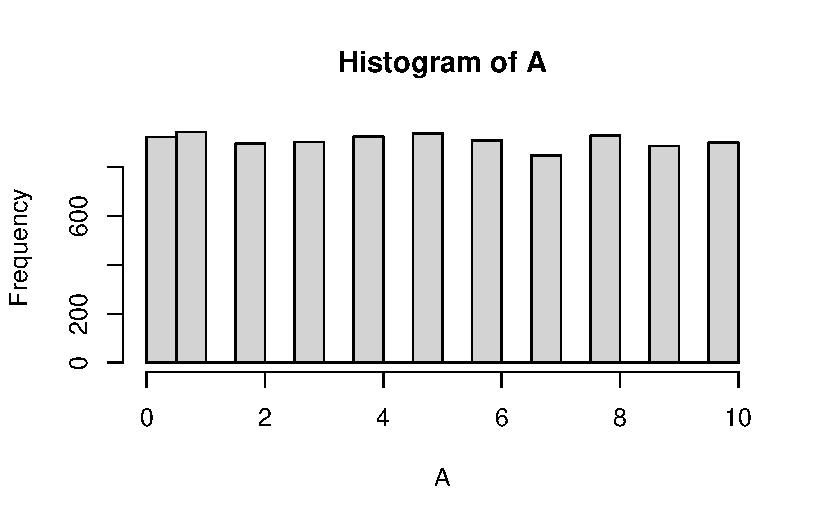
\includegraphics[keepaspectratio]{App_B-distribution_files/figure-pdf/unnamed-chunk-1-1.pdf}}

\begin{Shaded}
\begin{Highlighting}[]
\CommentTok{\# Sample mean and variance}
\FunctionTok{mean}\NormalTok{(A)}
\end{Highlighting}
\end{Shaded}

\begin{verbatim}
[1] 4.9627
\end{verbatim}

\begin{Shaded}
\begin{Highlighting}[]
\FunctionTok{var}\NormalTok{(A)}
\end{Highlighting}
\end{Shaded}

\begin{verbatim}
[1] 10.00951
\end{verbatim}

\begin{Shaded}
\begin{Highlighting}[]
\CommentTok{\# Theoretical mean of Uniform(a, b) is (a + b)/2}
\NormalTok{(mean.est }\OtherTok{\textless{}{-}}\NormalTok{ (}\FunctionTok{min}\NormalTok{(A) }\SpecialCharTok{+} \FunctionTok{max}\NormalTok{(A)) }\SpecialCharTok{/} \DecValTok{2}\NormalTok{)}
\end{Highlighting}
\end{Shaded}

\begin{verbatim}
[1] 5
\end{verbatim}

\begin{Shaded}
\begin{Highlighting}[]
\CommentTok{\# Theoretical variance of Uniform(a, b) is (b {-} a)\^{}2 / 12}
\NormalTok{(var.est }\OtherTok{\textless{}{-}}\NormalTok{ ((}\FunctionTok{max}\NormalTok{(A) }\SpecialCharTok{{-}} \FunctionTok{min}\NormalTok{(A) }\SpecialCharTok{+} \DecValTok{1}\NormalTok{ )}\SpecialCharTok{\^{}}\DecValTok{2} \SpecialCharTok{{-}}\DecValTok{1}\NormalTok{ ) }\SpecialCharTok{/} \DecValTok{12}\NormalTok{)}
\end{Highlighting}
\end{Shaded}

\begin{verbatim}
[1] 10
\end{verbatim}

\subsection{Bernoulli Distribution}\label{bernoulli-distribution}

There are only 2 possible outcomes in an experiment: \emph{True} and
\emph{False}, with probabiltiy \(\theta\) and \(1-\theta\),
respectively, the random variable \(X\) follows a Bernoulli
distribution, denoted by \(X\sim \text{Bern}(\theta)\). The probabiltiy
distribution has probablity mass function as
\[f(x) = \theta^x (1-\theta)^{1-x},\quad x=0,1.\]

Note that Bernoulli distribution is a special case of the Binomial
distribution with \(n=1\).

\subsubsection{Implementation in R}\label{implementation-in-r-1}

\begin{Shaded}
\begin{Highlighting}[]
\FunctionTok{rbinom}\NormalTok{(}\DecValTok{10}\NormalTok{, }\DecValTok{1}\NormalTok{, }\FloatTok{0.7}\NormalTok{) }\CommentTok{\# 0.7 is the probability of success}
\end{Highlighting}
\end{Shaded}

\subsection{Binomial Distribution}\label{binomial-distribution}

Bernoulli trials (experiment where a Bernoulli Distribution applies) are
not very realistic in real-life scenario. In statistics, repeated
experiments are important. When the experiments is repeated, \(\theta\)
is the same for each of the trials, and the trials are independent, and
they are only two mutually excludes outcomes (T, and F), we can model
this using the \emph{Binomial Distribution}. If \(X\) follows the
Binomial Distribution, it has a probablitliy mass function as
\[b(x ; n, \theta)=\binom{n}{x} \theta^x(1-\theta)^{n-x}, x=0,1,2,3, \ldots, n.\]

The Binomial Distribution is useful to predict the number of heads in
\(n\) coin tosses, the number of people infected with a disease in a
certain population of known size, etc. The parameters \(n\) and
\(\theta\) must be given.

The mean and variance of the Binomial Distribution \[
\mathbb{E}X = n\theta,\quad \text{and}\quad \mathbb{V}ar(X) = n\theta(1-\theta).\]

\subsubsection{Implementation in R}\label{implementation-in-r-2}

\begin{Shaded}
\begin{Highlighting}[]
\NormalTok{X }\OtherTok{=} \FunctionTok{rbinom}\NormalTok{(}\DecValTok{10000}\NormalTok{, }\DecValTok{4}\NormalTok{, }\AttributeTok{prob =} \FloatTok{0.3}\NormalTok{)}
\FunctionTok{mean}\NormalTok{(X }\SpecialCharTok{==} \DecValTok{1}\NormalTok{)}
\end{Highlighting}
\end{Shaded}

\begin{verbatim}
[1] 0.4053
\end{verbatim}

\begin{Shaded}
\begin{Highlighting}[]
\FunctionTok{mean}\NormalTok{(X }\SpecialCharTok{\textgreater{}} \DecValTok{1}\NormalTok{)}
\end{Highlighting}
\end{Shaded}

\begin{verbatim}
[1] 0.3482
\end{verbatim}

\subsection{Geometric Distribution}\label{geometric-distribution}

If we are interested in the number of trials until the first success,
then this is modeled by the geometric distribution. A random variable
\(X\) follows a geometric distribution if and only if its probability
distribution is given by: \[
g(x;\theta) = \theta (1 - \theta)^{\,x-1}, \quad x = 1,2,3,\ldots
\]

\begin{Shaded}
\begin{Highlighting}[]
\CommentTok{\# Function to generate n samples from Geometric(p)}
\NormalTok{geom.gener }\OtherTok{\textless{}{-}} \ControlFlowTok{function}\NormalTok{(n, p) \{}
\NormalTok{  tmp }\OtherTok{\textless{}{-}} \ConstantTok{NULL}
  \ControlFlowTok{for}\NormalTok{ (i }\ControlFlowTok{in} \DecValTok{1}\SpecialCharTok{:}\NormalTok{n) \{}
\NormalTok{    u }\OtherTok{\textless{}{-}} \FunctionTok{runif}\NormalTok{(}\DecValTok{1}\NormalTok{)  }\CommentTok{\# Uniform(0,1)}
\NormalTok{    x }\OtherTok{\textless{}{-}} \DecValTok{1}
\NormalTok{    p.x }\OtherTok{\textless{}{-}}\NormalTok{ p}
\NormalTok{    sum }\OtherTok{\textless{}{-}}\NormalTok{ p.x}
    
    \ControlFlowTok{while}\NormalTok{ (sum }\SpecialCharTok{\textless{}}\NormalTok{ u) \{}
\NormalTok{      x }\OtherTok{\textless{}{-}}\NormalTok{ x }\SpecialCharTok{+} \DecValTok{1}
\NormalTok{      p.x }\OtherTok{\textless{}{-}}\NormalTok{ p.x }\SpecialCharTok{*}\NormalTok{ (}\DecValTok{1} \SpecialCharTok{{-}}\NormalTok{ p)}
\NormalTok{      sum }\OtherTok{\textless{}{-}}\NormalTok{ sum }\SpecialCharTok{+}\NormalTok{ p.x}
\NormalTok{    \}}
    
\NormalTok{    tmp }\OtherTok{\textless{}{-}} \FunctionTok{c}\NormalTok{(tmp, x)}
\NormalTok{  \}}
  \FunctionTok{return}\NormalTok{(tmp)}
\NormalTok{\}}

\CommentTok{\# Example: generate 100,000 samples with p = 0.75}
\NormalTok{x }\OtherTok{\textless{}{-}} \FunctionTok{geom.gener}\NormalTok{(}\DecValTok{100000}\NormalTok{, }\FloatTok{0.75}\NormalTok{)}

\CommentTok{\# Relative frequencies}
\FunctionTok{table}\NormalTok{(x) }\SpecialCharTok{/} \DecValTok{100000}
\end{Highlighting}
\end{Shaded}

\begin{verbatim}
x
      1       2       3       4       5       6       7       8       9 
0.74828 0.18913 0.04680 0.01179 0.00317 0.00063 0.00014 0.00005 0.00001 
\end{verbatim}

\begin{Shaded}
\begin{Highlighting}[]
\CommentTok{\# OR }
\NormalTok{X }\OtherTok{=} \FunctionTok{rgeom}\NormalTok{(}\DecValTok{100000}\NormalTok{, }\AttributeTok{prob=} \FloatTok{0.75}\NormalTok{)}
\FunctionTok{table}\NormalTok{(X)}\SpecialCharTok{/}\DecValTok{100000}
\end{Highlighting}
\end{Shaded}

\begin{verbatim}
X
      0       1       2       3       4       5       6       7       8 
0.74811 0.18907 0.04773 0.01132 0.00282 0.00064 0.00024 0.00005 0.00002 
\end{verbatim}

Do you notice the difference between the two functions? R starts the
geometric distribution at \(x = 0\) and not \(x = 1\). We can check that
both of these simulate the same distribution by checking a qqplot.

\begin{Shaded}
\begin{Highlighting}[]
\CommentTok{\# Correlation between points in QQ plot}
\FunctionTok{cor}\NormalTok{(}\FunctionTok{qqplot}\NormalTok{(x, X }\SpecialCharTok{+} \DecValTok{1}\NormalTok{)}\SpecialCharTok{$}\NormalTok{x, }\FunctionTok{qqplot}\NormalTok{(x, X }\SpecialCharTok{+} \DecValTok{1}\NormalTok{)}\SpecialCharTok{$}\NormalTok{y)}
\end{Highlighting}
\end{Shaded}

\pandocbounded{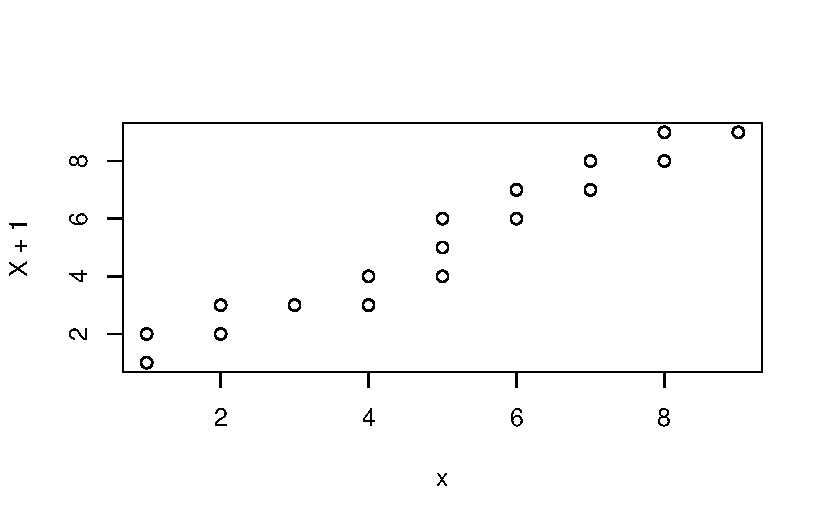
\includegraphics[keepaspectratio]{App_B-distribution_files/figure-pdf/unnamed-chunk-4-1.pdf}}

\begin{verbatim}
[1] 0.998222
\end{verbatim}

\subsection{Hypergeometric
Distribution}\label{hypergeometric-distribution}

The motivating question: what happens in a Binomial setting when our
trials are NOT independent? In other words, what happens when we sample
without replacement?

Consider a set of N elements, of which M are successes. We are
interested in obtaining X successes in n trials. This situation is
modeled by the Hypergeometric Distribution, which has pdf:

\[h(x,n,M,N) = \frac{\binom{M}{x}\binom{N-M}{n-x}}{\binom{N}{n}}, \quad x = 0,1,2,\ldots,n\]

The mean and the variance are \[\mathbb{E}X = \frac{nM}{N}, \qquad
\mathbb{V}ar(X) = \frac{nM(N-M)(N-n)}{N^2(N-1)}.\]

\subsubsection{Implementation in R}\label{implementation-in-r-3}

\begin{Shaded}
\begin{Highlighting}[]
\CommentTok{\# Define population: 12 ones and 13 zeros}
\NormalTok{x }\OtherTok{\textless{}{-}} \FunctionTok{c}\NormalTok{(}\DecValTok{1}\NormalTok{,}\DecValTok{1}\NormalTok{,}\DecValTok{1}\NormalTok{,}\DecValTok{1}\NormalTok{,}\DecValTok{1}\NormalTok{,}\DecValTok{1}\NormalTok{,}\DecValTok{1}\NormalTok{,}\DecValTok{1}\NormalTok{,}\DecValTok{1}\NormalTok{,}\DecValTok{1}\NormalTok{,}\DecValTok{0}\NormalTok{,}\DecValTok{0}\NormalTok{,}\DecValTok{0}\NormalTok{,}\DecValTok{0}\NormalTok{,}\DecValTok{0}\NormalTok{,}\DecValTok{0}\NormalTok{,}\DecValTok{0}\NormalTok{,}\DecValTok{0}\NormalTok{,}\DecValTok{0}\NormalTok{,}\DecValTok{0}\NormalTok{,}\DecValTok{0}\NormalTok{,}\DecValTok{0}\NormalTok{,}\DecValTok{0}\NormalTok{,}\DecValTok{0}\NormalTok{,}\DecValTok{0}\NormalTok{)}

\CommentTok{\# Take one sample of size 8 without replacement}
\NormalTok{s1 }\OtherTok{\textless{}{-}} \FunctionTok{sample}\NormalTok{(x, }\DecValTok{8}\NormalTok{, }\AttributeTok{replace =} \ConstantTok{FALSE}\NormalTok{)}
\NormalTok{s1}
\end{Highlighting}
\end{Shaded}

\begin{verbatim}
[1] 1 0 0 1 0 1 1 0
\end{verbatim}

\begin{Shaded}
\begin{Highlighting}[]
\CommentTok{\# Count how many ones in that sample}
\FunctionTok{sum}\NormalTok{(s1 }\SpecialCharTok{==} \DecValTok{1}\NormalTok{)}
\end{Highlighting}
\end{Shaded}

\begin{verbatim}
[1] 4
\end{verbatim}

\begin{Shaded}
\begin{Highlighting}[]
\CommentTok{\# Repeat the sampling 10,000 times}
\NormalTok{y }\OtherTok{\textless{}{-}} \FunctionTok{replicate}\NormalTok{(}\DecValTok{10000}\NormalTok{, }\FunctionTok{sample}\NormalTok{(x, }\DecValTok{8}\NormalTok{, }\AttributeTok{replace =} \ConstantTok{FALSE}\NormalTok{))}

\CommentTok{\# Column sums = number of ones in each sample}
\NormalTok{z }\OtherTok{\textless{}{-}} \FunctionTok{colSums}\NormalTok{(y)}

\CommentTok{\# Histogram of simulated distribution}
\FunctionTok{hist}\NormalTok{(z)}
\end{Highlighting}
\end{Shaded}

\pandocbounded{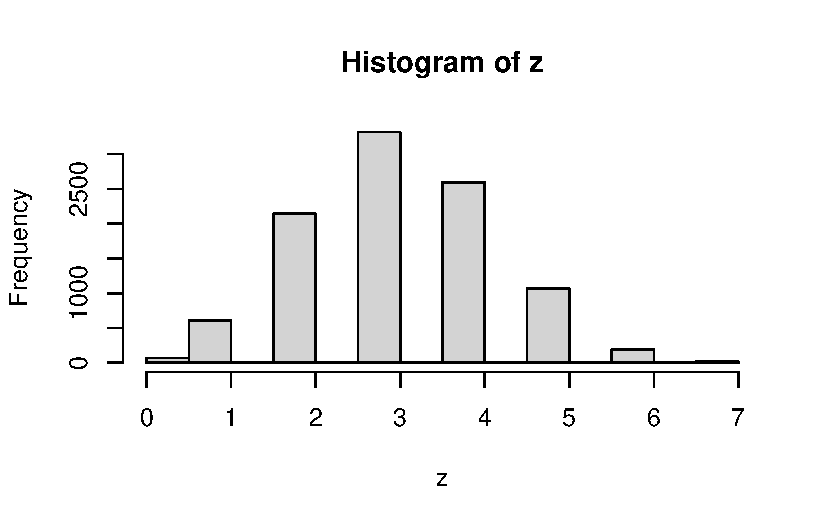
\includegraphics[keepaspectratio]{App_B-distribution_files/figure-pdf/unnamed-chunk-5-1.pdf}}

\begin{Shaded}
\begin{Highlighting}[]
\CommentTok{\# Probability of getting exactly 5 ones}
\FunctionTok{mean}\NormalTok{(z }\SpecialCharTok{==} \DecValTok{5}\NormalTok{)}
\end{Highlighting}
\end{Shaded}

\begin{verbatim}
[1] 0.107
\end{verbatim}

\begin{Shaded}
\begin{Highlighting}[]
\CommentTok{\# Sample mean and variance of distribution}
\FunctionTok{mean}\NormalTok{(z)}
\end{Highlighting}
\end{Shaded}

\begin{verbatim}
[1] 3.1804
\end{verbatim}

\begin{Shaded}
\begin{Highlighting}[]
\FunctionTok{var}\NormalTok{(z)}
\end{Highlighting}
\end{Shaded}

\begin{verbatim}
[1] 1.367393
\end{verbatim}

\subsection{Poisson Distribution}\label{poisson-distribution}

Calculating Binomial probabilities when \(n\) is large can be highly
tedious and time-consuming. As \(n\) approaches infinity and the
probability of success approaches \(0\), where \(n\theta\) remains
fixed. We can define \(n\theta = \lambda\), and obtain the distribution
called Poisson.

A random variable X has the Poisson Distribution if and only if its
probability distribution is given by:

\[P(x;\lambda) = \frac{\lambda^x e^{-\lambda}}{x!}, \quad x = 0,1,2,\ldots\]

\begin{Shaded}
\begin{Highlighting}[]
\CommentTok{\# Generate 10,000 samples from Poisson(λ = 2)}
\NormalTok{X }\OtherTok{\textless{}{-}} \FunctionTok{rpois}\NormalTok{(}\DecValTok{10000}\NormalTok{, }\DecValTok{2}\NormalTok{)}

\CommentTok{\# Histogram of simulated data}
\FunctionTok{hist}\NormalTok{(X)}
\end{Highlighting}
\end{Shaded}

\pandocbounded{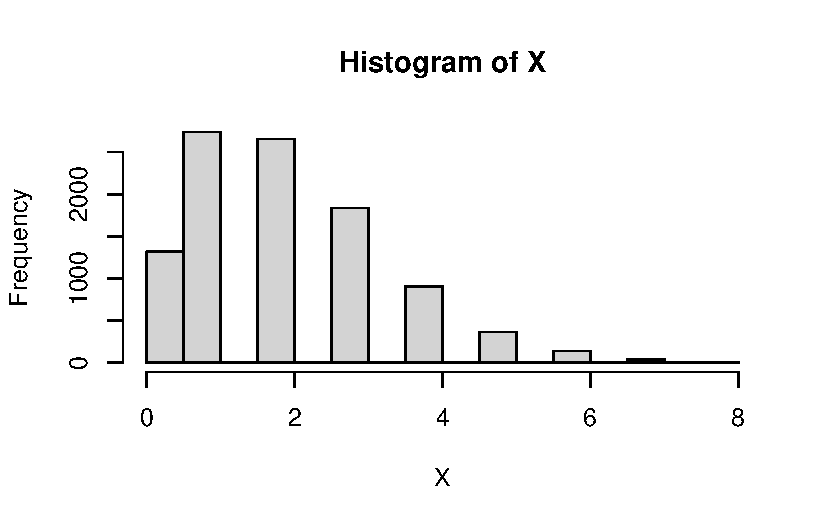
\includegraphics[keepaspectratio]{App_B-distribution_files/figure-pdf/poisson-1.pdf}}

\begin{Shaded}
\begin{Highlighting}[]
\CommentTok{\# Probability that X \textgreater{} 3 (estimated by simulation)}
\FunctionTok{mean}\NormalTok{(X }\SpecialCharTok{\textgreater{}} \DecValTok{3}\NormalTok{)}
\end{Highlighting}
\end{Shaded}

\begin{verbatim}
[1] 0.1456
\end{verbatim}

\begin{Shaded}
\begin{Highlighting}[]
\CommentTok{\# Probability that X = 0 (estimated by simulation)}
\FunctionTok{mean}\NormalTok{(X }\SpecialCharTok{==} \DecValTok{0}\NormalTok{)}
\end{Highlighting}
\end{Shaded}

\begin{verbatim}
[1] 0.1318
\end{verbatim}

\begin{Shaded}
\begin{Highlighting}[]
\CommentTok{\# Theoretical probability that X = 0}
\FunctionTok{exp}\NormalTok{(}\SpecialCharTok{{-}}\DecValTok{2}\NormalTok{)}
\end{Highlighting}
\end{Shaded}

\begin{verbatim}
[1] 0.1353353
\end{verbatim}

\begin{Shaded}
\begin{Highlighting}[]
\CommentTok{\# Sample mean and variance of simulated distribution}
\FunctionTok{mean}\NormalTok{(X)}
\end{Highlighting}
\end{Shaded}

\begin{verbatim}
[1] 2.0172
\end{verbatim}

\begin{Shaded}
\begin{Highlighting}[]
\FunctionTok{var}\NormalTok{(X)}
\end{Highlighting}
\end{Shaded}

\begin{verbatim}
[1] 2.025707
\end{verbatim}

The mean and variance of the Poisson distribution are

\[\mathbb{E}X = \lambda, \qquad \mathbb{V}ar(X) = \lambda\]

The Poisson distribution is derived as the limiting case of the Binomial
(with the above mentioned restrictions) BUT there are many more
applications. It models:

\begin{enumerate}
\def\labelenumi{\arabic{enumi}.}
\item
  Number of successes to occur in a given time period
\item
  Number of telephone calls received in a given time
\item
  Number of misprints on a page
\item
  Number of customers entering a bank during various intervals of time
\end{enumerate}

⸻

We are now moving onto the \emph{continuous distributions} that play an
important role in Statistical Theory.

\section{Continuous Distributions}\label{continuous-distributions}

\subsection{Uniform Distribution}\label{uniform-distribution}

Similar to the discrete uniform distribution except all values within an
interval have equal probability. The parameters of the Uniform Density
are \alpha and \operatorname{Beta} (\alpha \textless{}
\operatorname{Beta}). The random variable X has the Uniform Distribution
if it is continuous and its probability density function is given by \[
f_X(x) =
\begin{cases}
\dfrac{1}{\operatorname{Beta}- \alpha}, & \alpha < x < \operatorname{Beta}, \\[1ex]
0, & \text{otherwise}.
\end{cases}
\]

The mean and variance of the Uniform Distribution are
\[\mathbb{E}X = \frac{\alpha + \operatorname{Beta}}{2},
\qquad
\mathbb{V}ar(X) = \frac{(\operatorname{Beta}- \alpha)^2}{12}.
\]

\subsubsection{Implementation in R}\label{implementation-in-r-4}

\begin{Shaded}
\begin{Highlighting}[]
\NormalTok{X }\OtherTok{\textless{}{-}} \FunctionTok{runif}\NormalTok{(}\DecValTok{1000}\NormalTok{)}

\CommentTok{\# Histogram of simulated data}
\FunctionTok{hist}\NormalTok{(X)}
\end{Highlighting}
\end{Shaded}

\pandocbounded{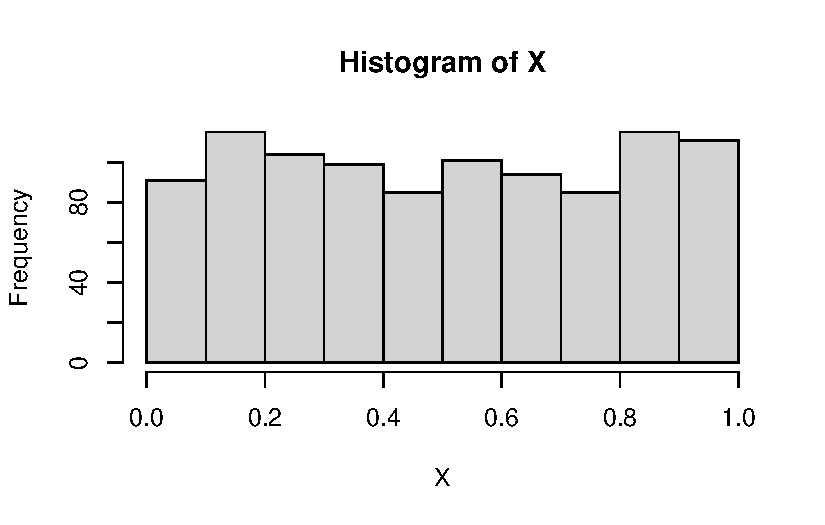
\includegraphics[keepaspectratio]{App_B-distribution_files/figure-pdf/Uniform-1.pdf}}

\begin{Shaded}
\begin{Highlighting}[]
\FunctionTok{mean}\NormalTok{(X);  }\FunctionTok{var}\NormalTok{(X)}
\end{Highlighting}
\end{Shaded}

\begin{verbatim}
[1] 0.5035435
\end{verbatim}

\begin{verbatim}
[1] 0.08632385
\end{verbatim}

\subsection{Gamma Distribution}\label{gamma-distribution}

The Gamma function is defined as
\[\Gamma(\alpha) = \int_{0}^{\infty} y^{\alpha - 1} e^{-y} \, dy.\]

For \(\alpha > 0\), \[
\Gamma(\alpha) = (\alpha - 1)\Gamma(\alpha - 1).\]

For any positive integer \(\alpha > 0\),
\[\Gamma(\alpha) = (\alpha - 1)!\]

A continuous random variable follows a Gamma Distribution if and only if
its probability density function is of the form \[f_X(x) =
\begin{cases}
\dfrac{1}{\operatorname{Beta}^{\alpha}\Gamma(\alpha)} x^{\alpha - 1} e^{-x/\operatorname{Beta}}, & x > 0, \\[2ex]
0, & \text{otherwise},
\end{cases}\] where \(\alpha, \operatorname{Beta}\) are positive. The
parameters \(\alpha\) and \(\operatorname{Beta}\) determine the shape of
the distribution. \(\alpha\) is called the shape parameter and
\(\operatorname{Beta}\) is called the scale parameter.

Theorem: The mean and variance of the Gamma Distribution are
\[\mathbb{E}X = \alpha \operatorname{Beta},
\qquad
\mathbb{V}ar(X) = \alpha \operatorname{Beta}^2\]

\subsubsection{Implementation in R}\label{implementation-in-r-5}

\begin{Shaded}
\begin{Highlighting}[]
\FunctionTok{rgamma}\NormalTok{(}\AttributeTok{n =} \DecValTok{10}\NormalTok{, }\AttributeTok{shape =} \DecValTok{10}\NormalTok{, }\AttributeTok{scale =} \DecValTok{3}\NormalTok{)}
\end{Highlighting}
\end{Shaded}

\subsection{Exponential Distribution}\label{exponential-distribution}

A special case of the Gamma Distribution arises when \(\alpha = 1\). To
differentiate it from the Gamma distribution, we also let
\(\operatorname{Beta}= \theta\). A continuous random variable follows an
Exponential Distribution if and only if its probability density function
is of the form: \[f_X(x) =
\begin{cases}
\dfrac{1}{\theta} e^{-x/\theta}, & x > 0, \\[2ex]
0, & \text{otherwise}.
\end{cases}\]

Exponential Distributions have many applications. One of them is a
waiting time until the first success of a Poisson process. In this
situation, it is often better to model the phenomenon in terms of a rate
parameter (i.e.~4 calls per week). Thus, the distribution of waiting
times becomes: \[
f_Y(y) =
\begin{cases}
\lambda e^{-\lambda y}, & y > 0, \\[2ex]
0, & \text{otherwise}.
\end{cases}\]

\subsubsection{Memoryless Property}\label{memoryless-property}

This is also called the \emph{Markov Property.} The distribution of
waiting time does not depend on how long you have already waited. In
other words: \[
P(X > s + t \mid X > t) = P(X > s).
\]

The mean and variance of the exponential distribution are
\[\mathbb{E}X = \theta,
\qquad
\mathbb{V}ar(X) = \theta^2.\]

\subsubsection{Implementation in R}\label{implementation-in-r-6}

\begin{Shaded}
\begin{Highlighting}[]
\CommentTok{\# Generate 1000 samples from Exponential(λ = 1)}
\NormalTok{X }\OtherTok{\textless{}{-}} \FunctionTok{rexp}\NormalTok{(}\DecValTok{1000}\NormalTok{)}
\FunctionTok{hist}\NormalTok{(X)}
\end{Highlighting}
\end{Shaded}

\pandocbounded{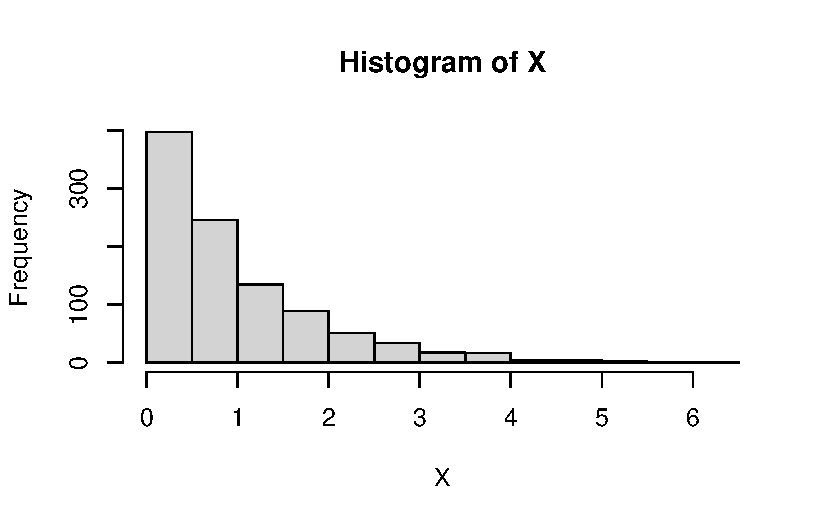
\includegraphics[keepaspectratio]{App_B-distribution_files/figure-pdf/unnamed-chunk-6-1.pdf}}

\begin{Shaded}
\begin{Highlighting}[]
\FunctionTok{mean}\NormalTok{(X); }\FunctionTok{var}\NormalTok{(X)}
\end{Highlighting}
\end{Shaded}

\begin{verbatim}
[1] 0.9746219
\end{verbatim}

\begin{verbatim}
[1] 0.9302842
\end{verbatim}

\subsection{Chi-Square Distribution}\label{chi-square-distribution}

There is another special form of the gamma distribution when
\(\alpha =\nu/2\) and \(\operatorname{Beta}= 2.
\nu\) is pronounced ``nu'' and is called the degrees of freedom.

A continuous random variable follows a Chi-Square Distribution if and
only if its probability density is given by \[f_X(x) =
\begin{cases}
\dfrac{1}{2^{\nu/2}\Gamma\!\left(\tfrac{\nu}{2}\right)} x^{\tfrac{\nu}{2} - 1} e^{-x/2}, & x > 0, \\[2ex]
0, & \text{otherwise}.
\end{cases}\]

The mean and variance of the Chi-Square Distribution are

\[\mathbb{E}X = \nu,
\qquad
\mathbb{V}ar(X) = 2\nu.\]

\begin{Shaded}
\begin{Highlighting}[]
\NormalTok{X }\OtherTok{\textless{}{-}} \FunctionTok{rchisq}\NormalTok{(}\DecValTok{1000}\NormalTok{, }\AttributeTok{df =} \DecValTok{5}\NormalTok{)}

\FunctionTok{hist}\NormalTok{(X)}
\end{Highlighting}
\end{Shaded}

\pandocbounded{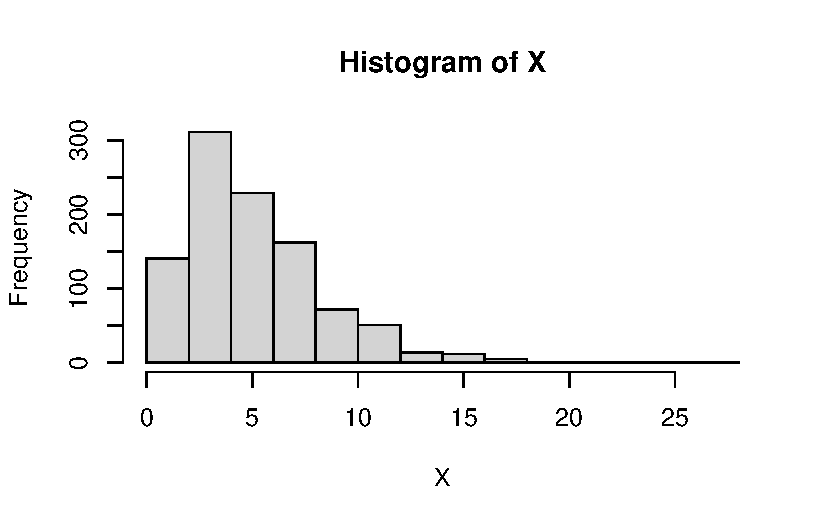
\includegraphics[keepaspectratio]{App_B-distribution_files/figure-pdf/chisq-1.pdf}}

\begin{Shaded}
\begin{Highlighting}[]
\FunctionTok{mean}\NormalTok{(X);  }\FunctionTok{var}\NormalTok{(X)}
\end{Highlighting}
\end{Shaded}

\begin{verbatim}
[1] 5.077642
\end{verbatim}

\begin{verbatim}
[1] 10.5748
\end{verbatim}

\subsection{Beta Distribution}\label{beta-distribution}

This is \textbf{Not} a special case of the Gamma distribution

The Beta function is defined as \[
B(\alpha, \operatorname{Beta}) = \frac{\Gamma(\alpha)\Gamma(\operatorname{Beta})}{\Gamma(\alpha + \operatorname{Beta})}
= \int_0^1 x^{\alpha - 1} (1-x)^{\operatorname{Beta}- 1} \, dx.\]

Like any probability density, the area underneath it must be equal to 1.
So, we can rearrange the above definition and write:
\[1 = \int_0^1 \frac{\Gamma(\alpha+\operatorname{Beta})}{\Gamma(\alpha)\Gamma(\operatorname{Beta})}
x^{\alpha-1} (1-x)^{\operatorname{Beta}-1} \, dx.\]

A continuous random variable follows a Beta Distribution if and only if
its probability density function is given by \[
f_X(x) =
\begin{cases}
\dfrac{\Gamma(\alpha+\operatorname{Beta})}{\Gamma(\alpha)\Gamma(\operatorname{Beta})}
x^{\alpha-1}(1-x)^{\operatorname{Beta}-1}, & 0 < x < 1, \\[2ex]
0, & \text{otherwise},
\end{cases}\] where \(\alpha > 0\), \(\operatorname{Beta}> 0\).

The mean and variance of the Beta Distribution are
\[\mathbb{E}X = \frac{\alpha}{\alpha + \operatorname{Beta}},
\qquad
\mathbb{V}ar(X) = \frac{\alpha \operatorname{Beta}}{(\alpha + \operatorname{Beta})^2 (\alpha + \operatorname{Beta}+ 1)}.
\]

\subsubsection{Implementation in R}\label{implementation-in-r-7}

\begin{Shaded}
\begin{Highlighting}[]
\FunctionTok{library}\NormalTok{(ggplot2)}

\CommentTok{\# Sequence of x values}
\NormalTok{t }\OtherTok{\textless{}{-}} \FunctionTok{seq}\NormalTok{(}\DecValTok{0}\NormalTok{, }\DecValTok{1}\NormalTok{, }\AttributeTok{by =} \FloatTok{0.01}\NormalTok{)}

\CommentTok{\# Create data frame with multiple Beta densities}
\NormalTok{df }\OtherTok{\textless{}{-}} \FunctionTok{data.frame}\NormalTok{(}
  \AttributeTok{x =} \FunctionTok{rep}\NormalTok{(t, }\DecValTok{4}\NormalTok{),}
  \AttributeTok{density =} \FunctionTok{c}\NormalTok{(}\FunctionTok{dbeta}\NormalTok{(t, }\DecValTok{2}\NormalTok{, }\DecValTok{2}\NormalTok{),}
              \FunctionTok{dbeta}\NormalTok{(t, }\DecValTok{2}\NormalTok{, }\DecValTok{8}\NormalTok{),}
              \FunctionTok{dbeta}\NormalTok{(t, }\DecValTok{8}\NormalTok{, }\DecValTok{2}\NormalTok{),}
              \FunctionTok{dbeta}\NormalTok{(t, }\DecValTok{1}\NormalTok{, }\DecValTok{1}\NormalTok{)),}
  \AttributeTok{dist =} \FunctionTok{factor}\NormalTok{(}\FunctionTok{rep}\NormalTok{(}\FunctionTok{c}\NormalTok{(}\StringTok{"Beta(2,2)"}\NormalTok{, }\StringTok{"Beta(2,8)"}\NormalTok{, }\StringTok{"Beta(8,2)"}\NormalTok{, }\StringTok{"Beta(1,1)"}\NormalTok{),}
                    \AttributeTok{each =} \FunctionTok{length}\NormalTok{(t)))}
\NormalTok{)}

\CommentTok{\# Plot with ggplot}
\FunctionTok{ggplot}\NormalTok{(df, }\FunctionTok{aes}\NormalTok{(}\AttributeTok{x =}\NormalTok{ x, }\AttributeTok{y =}\NormalTok{ density, }\AttributeTok{color =}\NormalTok{ dist)) }\SpecialCharTok{+}
  \FunctionTok{geom\_line}\NormalTok{(}\AttributeTok{size =} \DecValTok{1}\NormalTok{) }\SpecialCharTok{+}
  \FunctionTok{labs}\NormalTok{(}\AttributeTok{x =} \StringTok{"X"}\NormalTok{, }\AttributeTok{y =} \StringTok{"Beta Density"}\NormalTok{, }\AttributeTok{title =} \StringTok{"Beta Distributions"}\NormalTok{) }\SpecialCharTok{+}
  \FunctionTok{theme\_minimal}\NormalTok{() }\SpecialCharTok{+}
  \FunctionTok{theme}\NormalTok{(}\AttributeTok{legend.title =} \FunctionTok{element\_blank}\NormalTok{())}
\end{Highlighting}
\end{Shaded}

\begin{verbatim}
Warning: Using `size` aesthetic for lines was deprecated in ggplot2 3.4.0.
i Please use `linewidth` instead.
\end{verbatim}

\pandocbounded{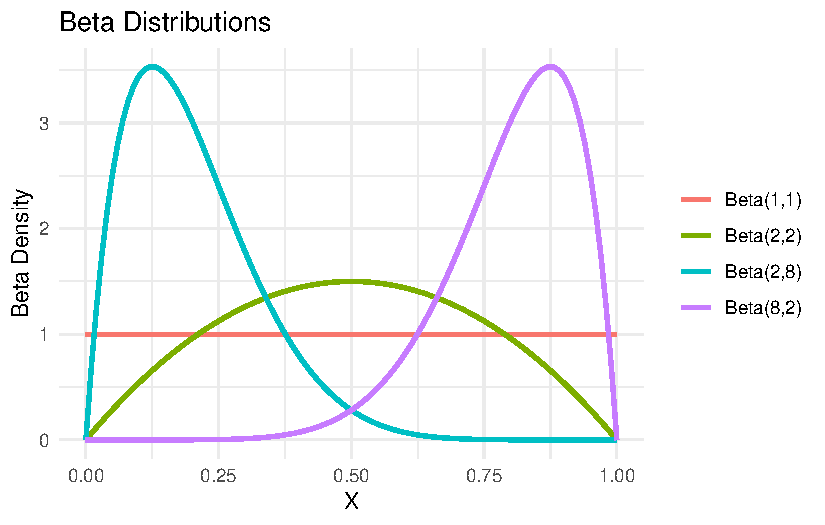
\includegraphics[keepaspectratio]{App_B-distribution_files/figure-pdf/beta-1.pdf}}

Q: What do you noitce about \(B(1,1)\)? What distribution is this?

The Beta distribution is related to the Binomial distribution when
computing maximum likelihood estimators !(We will make use of this
property later when we do Bayesian analysis.)
\[\text{Beta}_{pdf}(p, n, k) = (n+1)\binom{n}{k} p^k (1-p)^{n-k},\]
where
\(p^\prime = \text{Binomial}_{pmf}(k,n,p), \quad k = \text{mode}(\text{Binomial}(n,p)).\)

To relate the binomial distribution to the scale and shape parameters of
the beta distribution:
\(\alpha = k + 1, \quad \operatorname{Beta}= n - \alpha + 2\).

\subsubsection{Implementation in R}\label{implementation-in-r-8}

Suppose we flip a coin 20 times and find that we have 8 heads. Thus, our
MLE is \(8/20 = 0.4\). We can visualize the likelihood function for this
scenario:

\begin{Shaded}
\begin{Highlighting}[]
\CommentTok{\# Likelihood plot using Binomial likelihood}
\NormalTok{likeli\_bino.plot }\OtherTok{\textless{}{-}} \ControlFlowTok{function}\NormalTok{(y, n) \{}
\NormalTok{  L }\OtherTok{\textless{}{-}} \ControlFlowTok{function}\NormalTok{(p) }\FunctionTok{dbinom}\NormalTok{(y, n, p)}
\NormalTok{  mle }\OtherTok{\textless{}{-}} \FunctionTok{optimize}\NormalTok{(L, }\AttributeTok{interval =} \FunctionTok{c}\NormalTok{(}\DecValTok{0}\NormalTok{, }\DecValTok{1}\NormalTok{), }\AttributeTok{maximum =} \ConstantTok{TRUE}\NormalTok{)}\SpecialCharTok{$}\NormalTok{max}
  
\NormalTok{  p }\OtherTok{\textless{}{-}}\NormalTok{ (}\DecValTok{1}\SpecialCharTok{:}\DecValTok{100}\NormalTok{) }\SpecialCharTok{/} \DecValTok{100}
  
  \CommentTok{\# Likelihood}
  \FunctionTok{plot}\NormalTok{(p, }\FunctionTok{L}\NormalTok{(p), }\AttributeTok{type =} \StringTok{"l"}\NormalTok{)}
  \FunctionTok{abline}\NormalTok{(}\AttributeTok{v =}\NormalTok{ mle)}
  
  \CommentTok{\# Log{-}likelihood}
  \FunctionTok{plot}\NormalTok{(p, }\FunctionTok{log}\NormalTok{(}\FunctionTok{L}\NormalTok{(p)), }\AttributeTok{type =} \StringTok{"l"}\NormalTok{, }\AttributeTok{main =} \StringTok{"binomial"}\NormalTok{)}
  \FunctionTok{abline}\NormalTok{(}\AttributeTok{v =}\NormalTok{ mle)}
\NormalTok{\}}
\FunctionTok{par}\NormalTok{(}\AttributeTok{mfrow =} \FunctionTok{c}\NormalTok{(}\DecValTok{1}\NormalTok{,}\DecValTok{1}\NormalTok{), }\AttributeTok{mar =} \FunctionTok{c}\NormalTok{(}\DecValTok{4}\NormalTok{,}\DecValTok{4}\NormalTok{,}\DecValTok{2}\NormalTok{,}\DecValTok{1}\NormalTok{))}
\FunctionTok{likeli\_bino.plot}\NormalTok{(}\DecValTok{8}\NormalTok{, }\DecValTok{20}\NormalTok{)}
\end{Highlighting}
\end{Shaded}

\pandocbounded{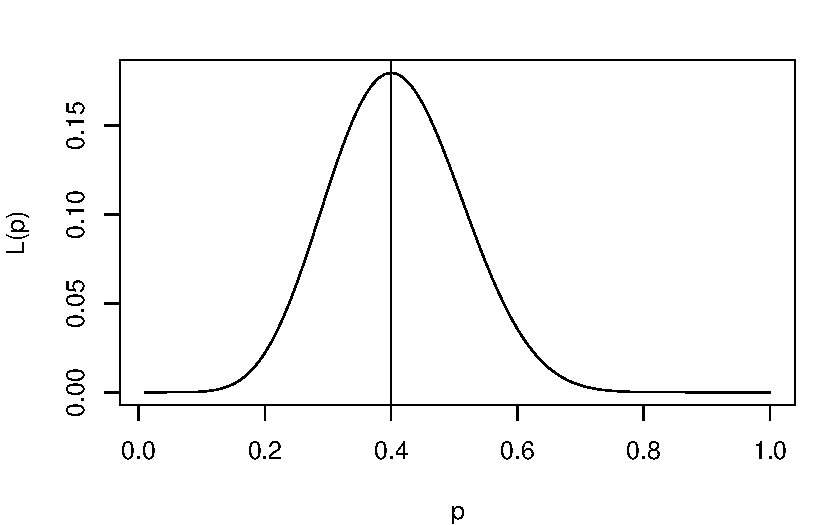
\includegraphics[keepaspectratio]{App_B-distribution_files/figure-pdf/beta-binomial-1.pdf}}

\pandocbounded{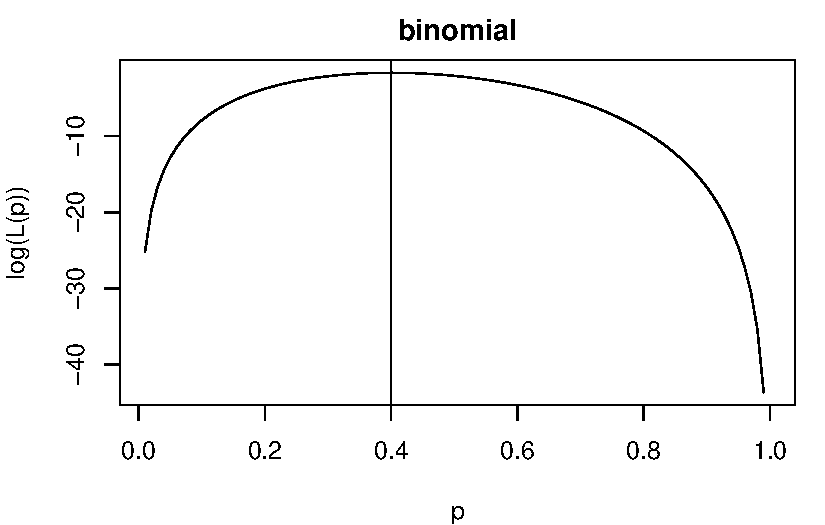
\includegraphics[keepaspectratio]{App_B-distribution_files/figure-pdf/beta-binomial-2.pdf}}

\begin{Shaded}
\begin{Highlighting}[]
\CommentTok{\# Likelihood plot using Beta distribution}
\NormalTok{likeli\_beta.plot }\OtherTok{\textless{}{-}} \ControlFlowTok{function}\NormalTok{(y, n) \{}
\NormalTok{  L }\OtherTok{\textless{}{-}} \ControlFlowTok{function}\NormalTok{(p) }\FunctionTok{dbeta}\NormalTok{(p, y }\SpecialCharTok{+} \DecValTok{1}\NormalTok{, n }\SpecialCharTok{{-}}\NormalTok{ (y }\SpecialCharTok{+} \DecValTok{1}\NormalTok{) }\SpecialCharTok{+} \DecValTok{2}\NormalTok{)}
\NormalTok{  mle }\OtherTok{\textless{}{-}} \FunctionTok{optimize}\NormalTok{(L, }\AttributeTok{interval =} \FunctionTok{c}\NormalTok{(}\DecValTok{0}\NormalTok{, }\DecValTok{1}\NormalTok{), }\AttributeTok{maximum =} \ConstantTok{TRUE}\NormalTok{)}\SpecialCharTok{$}\NormalTok{max}
  
\NormalTok{  p }\OtherTok{\textless{}{-}}\NormalTok{ (}\DecValTok{1}\SpecialCharTok{:}\DecValTok{100}\NormalTok{) }\SpecialCharTok{/} \DecValTok{100}
  
  \CommentTok{\# Likelihood}
  \FunctionTok{plot}\NormalTok{(p, }\FunctionTok{L}\NormalTok{(p), }\AttributeTok{type =} \StringTok{"l"}\NormalTok{)}
  \FunctionTok{abline}\NormalTok{(}\AttributeTok{v =}\NormalTok{ mle)}
  
  \CommentTok{\# Log{-}likelihood}
  \FunctionTok{plot}\NormalTok{(p, }\FunctionTok{log}\NormalTok{(}\FunctionTok{L}\NormalTok{(p)), }\AttributeTok{type =} \StringTok{"l"}\NormalTok{, }\AttributeTok{main =} \StringTok{"Beta"}\NormalTok{)}
  \FunctionTok{abline}\NormalTok{(}\AttributeTok{v =}\NormalTok{ mle)}
  
\NormalTok{  mle}
\NormalTok{\}}
\FunctionTok{likeli\_beta.plot}\NormalTok{(}\DecValTok{8}\NormalTok{, }\DecValTok{20}\NormalTok{)}
\end{Highlighting}
\end{Shaded}

\pandocbounded{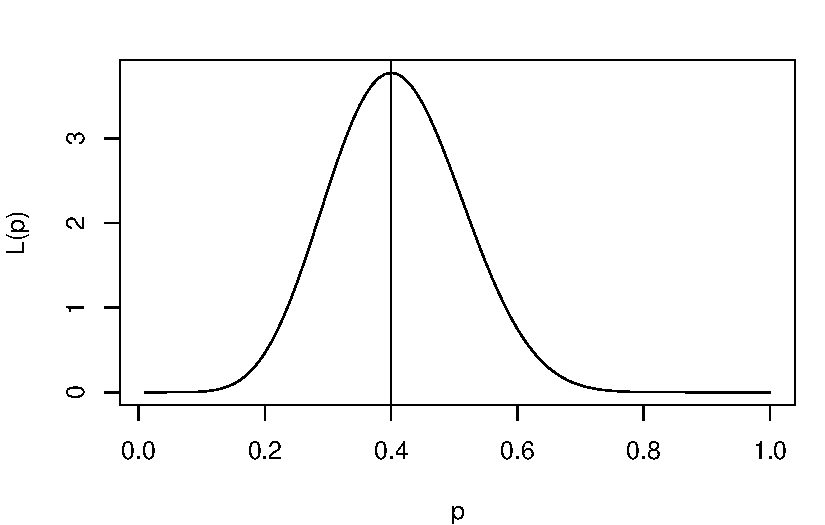
\includegraphics[keepaspectratio]{App_B-distribution_files/figure-pdf/beta-binomial-3.pdf}}

\pandocbounded{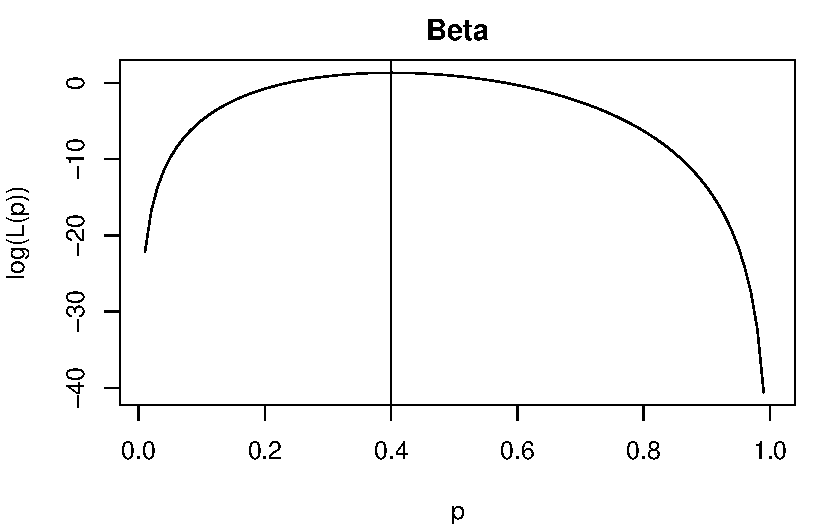
\includegraphics[keepaspectratio]{App_B-distribution_files/figure-pdf/beta-binomial-4.pdf}}

\begin{verbatim}
[1] 0.3999996
\end{verbatim}

\begin{Shaded}
\begin{Highlighting}[]
\NormalTok{overlay.likeli }\OtherTok{\textless{}{-}} \ControlFlowTok{function}\NormalTok{(y, n) \{}
  \CommentTok{\# Binomial likelihood}
\NormalTok{  L\_binom }\OtherTok{\textless{}{-}} \ControlFlowTok{function}\NormalTok{(p) }\FunctionTok{dbinom}\NormalTok{(y, n, p)}
  
  \CommentTok{\# Beta likelihood (with α = y+1, β = n{-}y+1)}
\NormalTok{  L\_beta }\OtherTok{\textless{}{-}} \ControlFlowTok{function}\NormalTok{(p) }\FunctionTok{dbeta}\NormalTok{(p, y }\SpecialCharTok{+} \DecValTok{1}\NormalTok{, n }\SpecialCharTok{{-}}\NormalTok{ y }\SpecialCharTok{+} \DecValTok{1}\NormalTok{)}
  
  \CommentTok{\# Sequence of p values}
\NormalTok{  p }\OtherTok{\textless{}{-}} \FunctionTok{seq}\NormalTok{(}\DecValTok{0}\NormalTok{, }\DecValTok{1}\NormalTok{, }\AttributeTok{length.out =} \DecValTok{200}\NormalTok{)}
  
  \CommentTok{\# Scale the beta likelihood so it’s comparable}
\NormalTok{  scale\_factor }\OtherTok{\textless{}{-}} \FunctionTok{max}\NormalTok{(}\FunctionTok{L\_binom}\NormalTok{(p)) }\SpecialCharTok{/} \FunctionTok{max}\NormalTok{(}\FunctionTok{L\_beta}\NormalTok{(p))}
  \FunctionTok{par}\NormalTok{(}\AttributeTok{mfrow=}\FunctionTok{c}\NormalTok{(}\DecValTok{1}\NormalTok{,}\DecValTok{1}\NormalTok{))}
  \CommentTok{\# Plot Binomial likelihood}
  \FunctionTok{plot}\NormalTok{(p, }\FunctionTok{L\_binom}\NormalTok{(p), }\AttributeTok{type =} \StringTok{"l"}\NormalTok{, }\AttributeTok{col =} \StringTok{"blue"}\NormalTok{, }\AttributeTok{lwd =} \DecValTok{2}\NormalTok{,}
       \AttributeTok{ylab =} \StringTok{"Likelihood"}\NormalTok{, }\AttributeTok{xlab =} \StringTok{"p"}\NormalTok{,}
       \AttributeTok{main =} \StringTok{"Binomial vs Beta Likelihood"}\NormalTok{)}
  
  \CommentTok{\# Add Beta likelihood (scaled for comparison)}
  \FunctionTok{lines}\NormalTok{(p, }\FunctionTok{L\_beta}\NormalTok{(p) }\SpecialCharTok{*}\NormalTok{ scale\_factor, }\AttributeTok{col =} \StringTok{"red"}\NormalTok{, }\AttributeTok{lwd =} \DecValTok{2}\NormalTok{, }\AttributeTok{lty =} \DecValTok{2}\NormalTok{)}
  
  \CommentTok{\# Add legend}
  \FunctionTok{legend}\NormalTok{(}\StringTok{"topright"}\NormalTok{,}
         \AttributeTok{legend =} \FunctionTok{c}\NormalTok{(}\StringTok{"Binomial Likelihood"}\NormalTok{, }\StringTok{"Beta Likelihood (scaled)"}\NormalTok{),}
         \AttributeTok{col =} \FunctionTok{c}\NormalTok{(}\StringTok{"blue"}\NormalTok{, }\StringTok{"red"}\NormalTok{),}
         \AttributeTok{lty =} \FunctionTok{c}\NormalTok{(}\DecValTok{1}\NormalTok{, }\DecValTok{2}\NormalTok{), }\AttributeTok{lwd =} \DecValTok{2}\NormalTok{)}
\NormalTok{\}}

\CommentTok{\# Example: 8 successes out of 20 trials}

\FunctionTok{overlay.likeli}\NormalTok{(}\DecValTok{8}\NormalTok{, }\DecValTok{20}\NormalTok{)}
\end{Highlighting}
\end{Shaded}

\pandocbounded{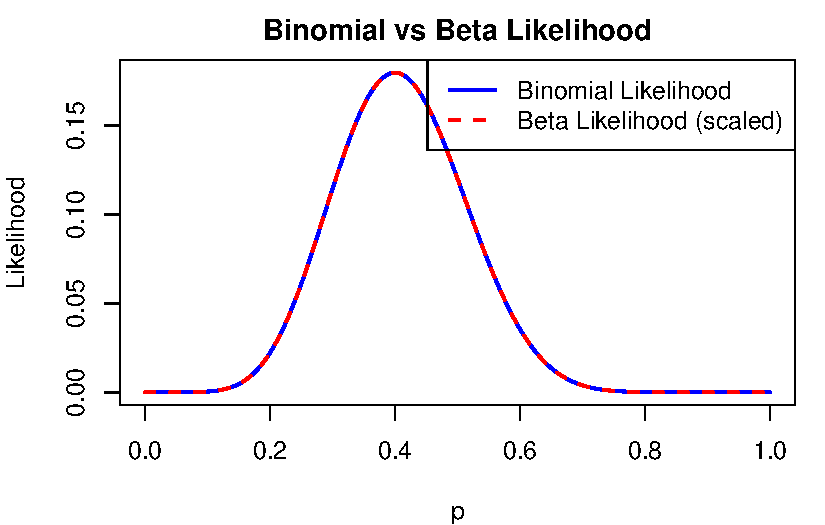
\includegraphics[keepaspectratio]{App_B-distribution_files/figure-pdf/beta-binomial-5.pdf}}

\subsection{Gaussian Distribution}\label{gaussian-distribution}

This is probably the most famous statistical distribution. It is defined
by its mean (\(\mu\)) and variance (\(\sigma^2\)). It is also known as
the Normal Distribution. A continuous random variable follows a Normal
Distribution if and only if its probability density function is given by

\[
f_X(x) =
\begin{cases}
\dfrac{1}{\sigma \sqrt{2\pi}} \exp\!\left( -\dfrac{(x - \mu)^2}{2\sigma^2} \right), & -\infty < x < \infty, \\[2ex]
0, & \text{otherwise}.
\end{cases}
\]

Note: The Standard Normal Distribution has density with
\(\mathbb{E}X = 0\) and \(\mathbb{V}ar(X) = 1\).

\begin{Shaded}
\begin{Highlighting}[]
\NormalTok{X }\OtherTok{\textless{}{-}} \FunctionTok{rnorm}\NormalTok{(}\DecValTok{1000}\NormalTok{, }\DecValTok{0}\NormalTok{, }\DecValTok{1}\NormalTok{)}
\FunctionTok{qqnorm}\NormalTok{(X)}
\end{Highlighting}
\end{Shaded}

\pandocbounded{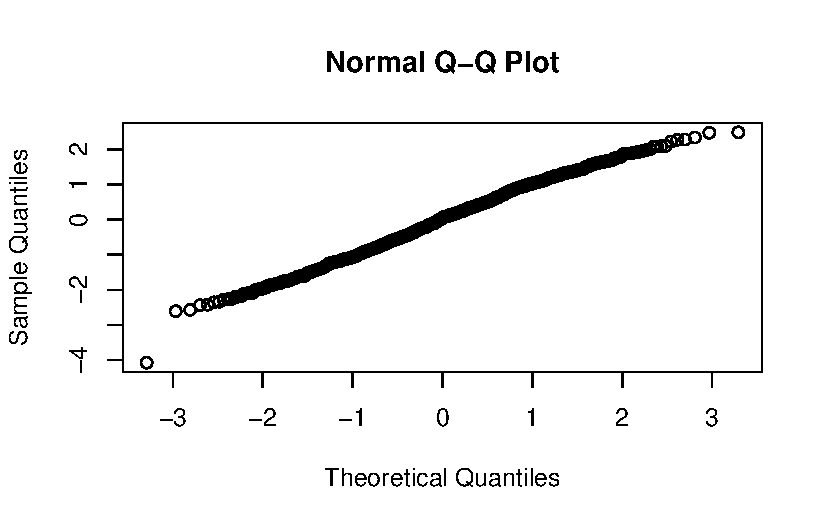
\includegraphics[keepaspectratio]{App_B-distribution_files/figure-pdf/normal-1.pdf}}

\begin{Shaded}
\begin{Highlighting}[]
\CommentTok{\# Approximate probabilities of being within 1, 2, 3 standard deviations}
\FunctionTok{mean}\NormalTok{(}\SpecialCharTok{{-}}\DecValTok{1} \SpecialCharTok{\textless{}}\NormalTok{ X }\SpecialCharTok{\&}\NormalTok{ X }\SpecialCharTok{\textless{}} \DecValTok{1}\NormalTok{)  }\CommentTok{\# \textasciitilde{} 68\%}
\end{Highlighting}
\end{Shaded}

\begin{verbatim}
[1] 0.655
\end{verbatim}

\begin{Shaded}
\begin{Highlighting}[]
\FunctionTok{mean}\NormalTok{(}\SpecialCharTok{{-}}\DecValTok{2} \SpecialCharTok{\textless{}}\NormalTok{ X }\SpecialCharTok{\&}\NormalTok{ X }\SpecialCharTok{\textless{}} \DecValTok{2}\NormalTok{)  }\CommentTok{\# \textasciitilde{} 95\%}
\end{Highlighting}
\end{Shaded}

\begin{verbatim}
[1] 0.971
\end{verbatim}

\begin{Shaded}
\begin{Highlighting}[]
\FunctionTok{mean}\NormalTok{(}\SpecialCharTok{{-}}\DecValTok{3} \SpecialCharTok{\textless{}}\NormalTok{ X }\SpecialCharTok{\&}\NormalTok{ X }\SpecialCharTok{\textless{}} \DecValTok{3}\NormalTok{)  }\CommentTok{\# \textasciitilde{} 99.7\%}
\end{Highlighting}
\end{Shaded}

\begin{verbatim}
[1] 0.999
\end{verbatim}

\subsection{T-Distribution}\label{t-distribution}

Another special distribution in statistical inference is the
\emph{Student's t-Distribution}. \[f_X(x) =
\begin{cases}
\dfrac{\Gamma\!\left(\tfrac{\nu+1}{2}\right)}
{\sqrt{\nu \pi}\,\Gamma\!\left(\tfrac{\nu}{2}\right)}
\left(1 + \dfrac{x^2}{\nu}\right)^{-\tfrac{\nu+1}{2}}, & -\infty < x < \infty, \\[2ex]
0, & \text{otherwise},
\end{cases}\] where \(\nu\) is the degrees of freedom. As
\(\nu \to \infty\), the pdf converges to the normal distribution.

\subsection{Implementation in R}\label{implementation-in-r-9}

\begin{Shaded}
\begin{Highlighting}[]
\NormalTok{my\_df }\OtherTok{\textless{}{-}} \DecValTok{5}
\NormalTok{X }\OtherTok{\textless{}{-}} \FunctionTok{rt}\NormalTok{(}\DecValTok{1000}\NormalTok{, }\AttributeTok{df =}\NormalTok{ my\_df)}

\FunctionTok{mean}\NormalTok{(X); }\FunctionTok{var}\NormalTok{(X)}
\end{Highlighting}
\end{Shaded}

\begin{verbatim}
[1] -0.05728994
\end{verbatim}

\begin{verbatim}
[1] 1.678916
\end{verbatim}

\begin{Shaded}
\begin{Highlighting}[]
\NormalTok{my\_df }\SpecialCharTok{/}\NormalTok{ (my\_df }\SpecialCharTok{{-}} \DecValTok{2}\NormalTok{)   }\CommentTok{\# Theoretical variance for df \textgreater{} 2}
\end{Highlighting}
\end{Shaded}

\begin{verbatim}
[1] 1.666667
\end{verbatim}

\subsection{Distribution Function
Technique}\label{distribution-function-technique}

For continuous random variables, a simple method for finding the
probability density of a function of random variables is to find the
distribution function and then differentiate to find the pdf.

To find an expression for the distribution function, let
\(Y = u(x_1, x_2, \ldots, x_n)\), where \(u\) is a function. Then,
\[F(Y) = P(Y \leq y) = P(u(x_1, x_2, \ldots, x_n) \leq y).\] Then,
\[f(y) = \frac{dF(Y)}{dy}.\]

Example:

\begin{Shaded}
\begin{Highlighting}[]
\CommentTok{\# Create sequence from 0 to 1}
\NormalTok{t }\OtherTok{\textless{}{-}} \FunctionTok{seq}\NormalTok{(}\DecValTok{0}\NormalTok{, }\DecValTok{1}\NormalTok{, }\AttributeTok{length =} \DecValTok{1000}\NormalTok{)}

\CommentTok{\# Define density function Y = 3 * (1 {-} t)\^{}2}
\NormalTok{Y }\OtherTok{\textless{}{-}} \DecValTok{3} \SpecialCharTok{*}\NormalTok{ (}\DecValTok{1} \SpecialCharTok{{-}}\NormalTok{ t)}\SpecialCharTok{\^{}}\DecValTok{2}

\CommentTok{\# Plot density}
\FunctionTok{plot}\NormalTok{(t, Y, }\AttributeTok{type =} \StringTok{"l"}\NormalTok{)}
\end{Highlighting}
\end{Shaded}

\pandocbounded{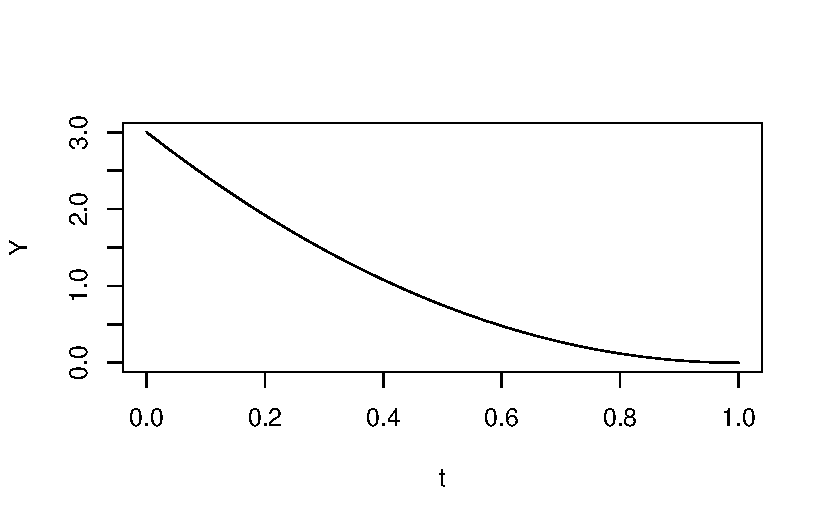
\includegraphics[keepaspectratio]{App_B-distribution_files/figure-pdf/unnamed-chunk-7-1.pdf}}

\begin{Shaded}
\begin{Highlighting}[]
\CommentTok{\# Sample from t with probability weights Y}
\NormalTok{Z }\OtherTok{\textless{}{-}} \FunctionTok{sample}\NormalTok{(t, }\DecValTok{10000}\NormalTok{, }\AttributeTok{replace =} \ConstantTok{TRUE}\NormalTok{, }\AttributeTok{prob =}\NormalTok{ Y)}

\CommentTok{\# Histogram of sampled values}
\FunctionTok{hist}\NormalTok{(Z, }\AttributeTok{freq =} \ConstantTok{FALSE}\NormalTok{)}

\CommentTok{\# Overlay the density curve}
\FunctionTok{lines}\NormalTok{(t, Y)}
\end{Highlighting}
\end{Shaded}

\pandocbounded{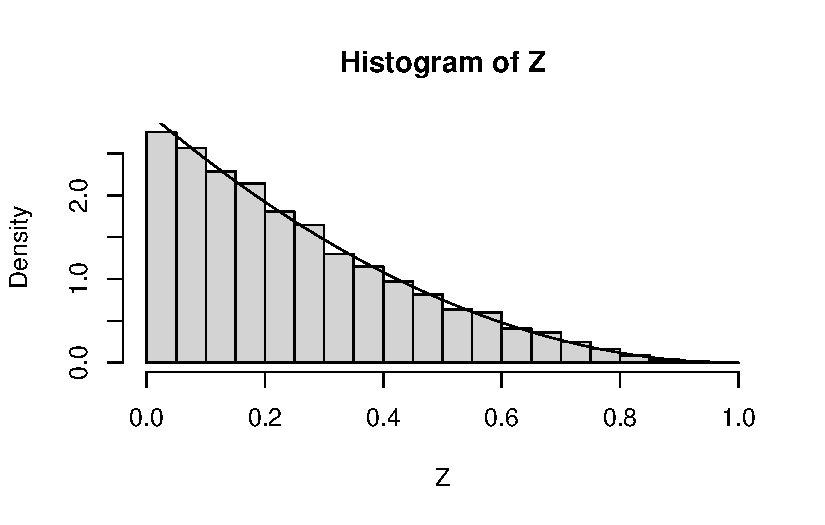
\includegraphics[keepaspectratio]{App_B-distribution_files/figure-pdf/unnamed-chunk-7-2.pdf}}

\begin{Shaded}
\begin{Highlighting}[]
\CommentTok{\# Apply transformation: X = (1 {-} Z)\^{}3}
\NormalTok{X.sample }\OtherTok{\textless{}{-}}\NormalTok{ (}\DecValTok{1} \SpecialCharTok{{-}}\NormalTok{ Z)}\SpecialCharTok{\^{}}\DecValTok{3}

\CommentTok{\# Histogram of transformed sample}
\FunctionTok{hist}\NormalTok{(X.sample)}
\end{Highlighting}
\end{Shaded}

\pandocbounded{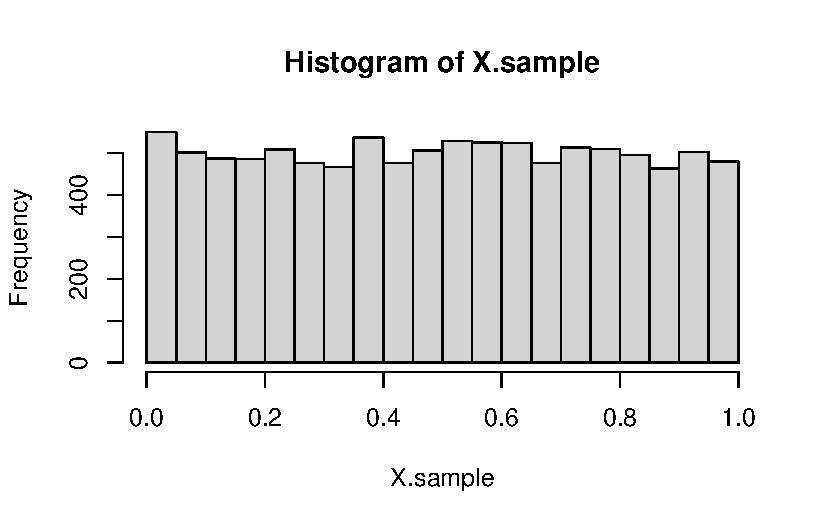
\includegraphics[keepaspectratio]{App_B-distribution_files/figure-pdf/unnamed-chunk-7-3.pdf}}

\begin{Shaded}
\begin{Highlighting}[]
\CommentTok{\# Compare with uniform distribution}
\NormalTok{U }\OtherTok{\textless{}{-}} \FunctionTok{runif}\NormalTok{(}\DecValTok{10000}\NormalTok{)}

\CommentTok{\# QQ{-}plot to check distributional similarity}
\FunctionTok{qqplot}\NormalTok{(U, X.sample)}
\end{Highlighting}
\end{Shaded}

\pandocbounded{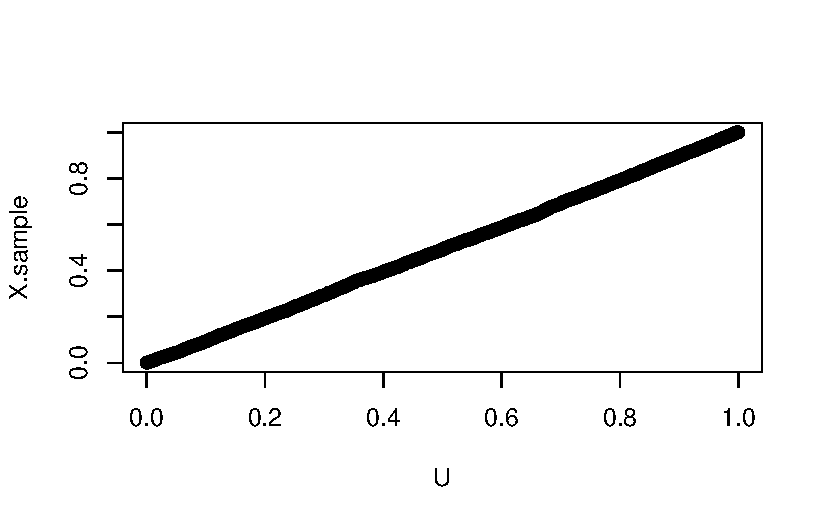
\includegraphics[keepaspectratio]{App_B-distribution_files/figure-pdf/unnamed-chunk-7-4.pdf}}

\begin{Shaded}
\begin{Highlighting}[]
\CommentTok{\# Correlation from QQ{-}plot}
\FunctionTok{cor}\NormalTok{(}\FunctionTok{qqplot}\NormalTok{(U, X.sample)}\SpecialCharTok{$}\NormalTok{x, }\FunctionTok{qqplot}\NormalTok{(U, X.sample)}\SpecialCharTok{$}\NormalTok{y)}
\end{Highlighting}
\end{Shaded}

\begin{verbatim}
[1] 0.9999307
\end{verbatim}

\begin{center}\rule{0.5\linewidth}{0.5pt}\end{center}

Special thanks to
Dr.~\href{https://cas.gsu.edu/profile/brian-pidgeon/}{Brian Pidgeon} who
kindly share the notes.

\chapter{Appendix: R Package}\label{appendix-r-package}

\newcommand{\E}{\mathbb{E}}
\newcommand{\var}{\mathbb{V}ar}

\begin{center}\rule{0.5\linewidth}{0.5pt}\end{center}

Resources

\begin{itemize}
\item
  \href{https://cran.r-project.org/web/packages/distributions/index.html}{CRAN
  page}
\item
  Wickham, H. and Bryan, J. \href{https://r-pkgs.org/}{R Package}.
\end{itemize}




\end{document}
